\documentclass[12pt,a4paper,oneside,openany]{book}
\usepackage[T1]{fontenc}
\usepackage[utf8]{inputenc}
\usepackage[english]{babel}
\usepackage{lmodern}
\usepackage[a4paper,left=32mm,right=27mm,top=28mm,bottom=29mm]{geometry}
\usepackage{amsmath,amssymb,bm}
\usepackage{graphicx,booktabs,longtable,array}
\usepackage{xcolor}
\usepackage{tikz}
\usetikzlibrary{arrows.meta,positioning,calc}
\usepackage{setspace}
\setstretch{1.18}
\usepackage{microtype}
\usepackage{fancyhdr}
\usepackage{caption}
\captionsetup{font=small,labelfont=bf}
\usepackage[numbers,sort&compress]{natbib}
\usepackage[hidelinks]{hyperref}
\hypersetup{pdftitle={Robust Dual-Arm Manipulation under Uncertainty via Convex Programming},pdfauthor={Lorenzo}}
\setlength{\headheight}{15pt}
\pagestyle{fancy}
\fancyhf{}
\fancyhead[L]{\small\nouppercase{\leftmark}}
\fancyfoot[C]{\thepage}
\renewcommand{\headrulewidth}{0.3pt}
\setcounter{tocdepth}{1}
\setcounter{secnumdepth}{2}
\setlength{\parindent}{1.4em}
\setlength{\parskip}{0pt}
\setlength{\emergencystretch}{2em}
\newcommand{\R}{\mathbb{R}}
\newcommand{\crossmat}[1]{[#1]_{\times}}
\newcommand{\norm}[1]{\left\lVert#1\right\rVert}
\newcommand{\diag}{\operatorname{diag}}
\newcommand{\tr}{\operatorname{tr}}
\newcommand{\CoM}{centre of mass}
\newcommand{\todo}[1]{\par\medskip\noindent\textbf{TODO --- #1}\par\medskip}
\newcommand{\sourcefile}[1]{\nolinkurl{#1}}
\newcommand{\thesisfigure}[4][0.92]{\begin{figure}[htbp]\centering\includegraphics[width=#1\textwidth]{figures/#2}\caption{#3}\label{#4}\end{figure}}
\newcommand{\vect}[1]{\bm{#1}}



% Complete these fields before submission. No identity or supervisor is inferred.
\newcommand{\ThesisTitle}{Robust Dual-Arm Manipulation under Uncertainty via Convex Programming}
\newcommand{\ThesisAuthor}{Lorenzo [surname]}
\newcommand{\StudentNumber}{[student number]}
\newcommand{\SupervisorName}{[supervisor]}
\newcommand{\CoSupervisorName}{[co-supervisor, if applicable]}
\newcommand{\AcademicYear}{[academic year]}


\begin{document}
\frontmatter
\hypersetup{pageanchor=false}
\begin{titlepage}
\centering
{\Large Universit\`a degli Studi di Genova\par}
\vspace{5mm}
{\large Polytechnic School\par}
\vspace{3mm}
{\normalsize Department of Informatics, Bioengineering,\par
Robotics and Systems Engineering (DIBRIS)\par}
\vspace{12mm}
{\large Master's Degree in Robotics Engineering\par}
\vspace{19mm}
{\LARGE\bfseries\ThesisTitle\par}
\vspace{9mm}
{\large Master's Thesis\par}
\vfill
\begin{minipage}[t]{0.46\textwidth}\raggedright
\textbf{Candidate}\par\ThesisAuthor\par
Student number: \StudentNumber
\end{minipage}\hfill
\begin{minipage}[t]{0.46\textwidth}\raggedright
\textbf{Supervisor}\par\SupervisorName\par\medskip
\textbf{Co-supervisor}\par\CoSupervisorName
\end{minipage}
\vspace{19mm}
\par Academic year \AcademicYear
\end{titlepage}
\hypersetup{pageanchor=true}
\chapter*{Abstract}
\addcontentsline{toc}{chapter}{Abstract}
Two arms can hold an object whose mass distribution is unknown, but the forces needed to hold it depend on both the load and the contacts that remain available. This thesis studies that dependence through a pipeline connecting haptic demonstrations, inertial estimation, contact force allocation and passive end-effector compliance.

Human demonstrations are recorded with two Haption interfaces controlling simulated hands. Each hand uses three discrete contact points arranged in a triangle. Their friction forces produce a resultant wrench and resist torsion through their lever arms. A task-parameterized Gaussian mixture model represents the joint distribution of gravity direction and bimanual wrist wrenches in world and object frames. Gaussian mixture regression provides an orientation-dependent mean and precision matrix for the control cost.

An autonomous lift estimates mass and the observable components of the centre of mass. Slow rotations in free space provide the additional directions needed to identify its vertical component. A second-order cone program allocates the six contact forces subject to unilateral compression, Coulomb friction and actuator limits. Equilibrium errors are penalized and reported separately from solver status. A force cost acts on every contact variable, including internal forces invisible to the resultant wrench.

The main experimental finding is that grip force is not a freely adjustable safety parameter. On a compliant wrist, additional squeeze can change the contact geometry and destroy a grasp. The same compliance also affects the torsional signal recorded during human demonstrations. These observations motivate a passive tri-pad whose conforming modes are separated from its load-bearing modes. The framework is then extended to progressively less regular geometries and to catalogue tetromino insertion using dynamic movement primitives. The latter is a distinct task with known mass and geometry and uncertain pose. A blind simulation campaign over 182 bodies finds that the floating-plate tri-pad, with no re-alignment controller, seats, estimates and places every jittered cube, while a fixed tri-pad needs a controller to seat and then loses the easiest bodies; on random polytopes the configurations are level. A colliding plate leaves the outcome nearly unchanged while invalidating the force model, and the learnt prior helps mostly through its weight, its shape adding a small benefit only on polytopes. Ongoing insertion campaigns are identified explicitly; they are not treated as completed validation.

\chapter*{Scope of this draft}
\addcontentsline{toc}{chapter}{Scope of this draft}
This manuscript is a source-checked working draft dated 30 September 2026. It distinguishes equations verified against the implementation, measurements documented in the project, and experiments still required. Numerical results from campaigns running at the time of writing are not final results. Visible TODO paragraphs identify the missing evidence. The intended final length is approximately 115 pages including front matter, references and appendices. The page allocation and completion checklist are maintained separately from the scientific text.



\tableofcontents
\listoffigures
\listoftables
\chapter*{Notation and conventions}
\addcontentsline{toc}{chapter}{Notation and conventions}
\begin{longtable}{@{}p{0.22\textwidth}p{0.71\textwidth}@{}}
\toprule Symbol & Meaning \\
\midrule\endhead
$W,B,G,H$ & World, body, grasp and haptic-device frames.\\
$R_{WB}$ & Rotation taking body coordinates into world coordinates.\\
$\vect g$ & World gravity acceleration, $(0,0,-9.81)^\top$ m/s$^2$.\\
$\hat{\vect g}_G$ & Unit gravity direction expressed in the grasp frame.\\
$m,\hat m$ & Actual mass and measured mass estimate.\\
$\vect c,\vect r_B$ & Moment reference point and CoM offset from it in body coordinates.\\
$\vect q$ & First mass moment, $m\vect r_B$.\\
$\crossmat{\vect a}$ & Matrix satisfying $\crossmat{\vect a}\vect b=\vect a\times\vect b$.\\
$\vect p_i,\vect n_i$ & Contact position and unit outward object-surface normal.\\
$\vect f_i$ & Force acting on the object at contact $i$.\\
$\lambda_i$ & Compressive magnitude $-\vect n_i^\top\vect f_i\geq0$.\\
$\mu,r_s$ & Friction coefficient and optional deterministic cone margin.\\
$\vect w$ & Bimanual wrist wrench $(F_L,\tau_L,F_R,\tau_R)\in\R^{12}$.\\
$\Sigma,Q$ & Conditional wrench covariance and precision $Q=\Sigma^{-1}$.\\
$S$ & Physical scaling matrix for the twelve wrench coordinates.\\
$\vect s_F,\vect s_T$ & Force and moment equilibrium slack.\\
$u,z$ & Command and environment state in the insertion model.\\
$\mathcal G$ & Reduced haptic metric in the insertion model.\\
$\Theta$ & DMP weights, three coordinates by twenty basis functions.\\
\bottomrule
\end{longtable}
Forces in the controller act on the object. A compressive force points into the surface, opposite to its outward normal. Moments are always specified about a stated pole. A rotation of a moment vector changes its coordinates; a change of pole also adds a force-dependent moment. These operations are kept distinct throughout the thesis.


\mainmatter
\chapter{Introduction}
\label{ch:introduction}

A closed carton gives little information about the distribution of its contents. Its dimensions may be visible while its mass and \CoM{} remain unknown. Two robots lifting it must supply the weight, balance its moments and maintain contact. A larger squeeze increases the friction capacity of a fixed Coulomb contact, but a real grasp need not remain fixed. The wrist can deflect, a pad can leave the surface, and the object can move relative to the hands. This thesis examines the consequences of that dependence rather than treating grip force as an unlimited reserve.

The experimental chain begins with a person manipulating a simulated object through two haptic interfaces. The demonstrations provide a model of how the two wrist wrenches vary together. The autonomous system then measures the load through a slow lift and, where necessary, rotates the object in the air to observe the remaining mass-distribution components. A convex program chooses contact forces that fit those estimates and the current contact geometry. Passive compliance is introduced when a rigid tool and a compliant wrist cannot provide both surface conformity and useful torsional measurements.

The central question is therefore practical: \emph{which aspects of a grasp must be measured, constrained or mechanically preserved before an optimized force allocation can be useful?} The human prior, the estimator and the optimizer each answer a different part of this question. None replaces the contact apparatus on which the other parts rely.

\section{Motivation in industrial handling}

Warehouse handling provides a direct example. Two cartons with the same external shape can contain a dense item near one corner or light contents distributed across the volume. A trajectory that is harmless for one carton can create a large gravitational moment for the other. A mass measurement alone cannot distinguish them. A vertical lift reveals the horizontal offset of the \CoM{}, while a change of orientation is required to identify the component initially parallel to gravity.

A second example is a return bin containing an irregular rigid object. A rough visual estimate may be adequate to bring two tools near opposite sides, but it does not establish three flat contact points per hand. The forces must be allocated on the contacts that actually exist. A detached pad cannot support a force simply because a nominal drawing places it on the surface. This motivates explicit contact masks and an end-effector able to accommodate small geometric mismatch.

A third example is replenishment into a crowded shelf. The grasp may be adequate in free space but inadequate once a neighbouring item opposes insertion. The hands must carry the additional interaction wrench. The trajectory can also matter: a small lateral movement or turn may allow the neighbouring item to move before the incoming part is lowered. This motivates the final insertion application. These examples identify possible uses of the framework; they are not claims of industrial deployment or throughput validation.

\section{Problem definition}

Consider a rigid body held by two hands, with three discrete contacts on each hand. In the blind handling task, its mass and \CoM{} are unknown. Geometry information is restricted to what the chosen experimental arm declares: an approximate size, a coarse visual representation or a known mesh used as a comparison. The controller receives estimated load parameters and measured contact information. Ground truth is reserved for constructing the simulation and calculating errors after execution.

The manipulation is slow enough for contact equilibrium to be an informative approximation. During lift estimation and wielding, the object is supported only by the two hands. No table, pivot or wall contributes to the load balance. The method assumes a known friction coefficient, rigid object mechanics and a contact measurement consistent with the sign and frame conventions of the model. The consequences of relaxing these assumptions are part of the discussion.

The final Tetris task changes the information available. Mass and geometry are taken from a declared catalogue; pose is uncertain. The wrench is then used to identify the offset between the planned grasp and the grasp that was obtained. Environmental contacts are deliberately present during staging and insertion. Results from this application are not pooled with blind inertial-estimation results.

\section{Research questions}

The work addresses four connected questions. First, can a haptic recording preserve the rotational signal that the force model is intended to learn? Second, what can be estimated from a vertical lift, and what requires an additional change of gravity direction? Third, how should the optimizer represent detached contacts, friction, effort and finite actuation? Fourth, how can the resulting grasp be used in an insertion task without replacing its finite force capacity with an ideal clamp?

The sequence matters. A statistical model trained on attenuated moments describes the recording apparatus as well as the person. An accurate optimizer can solve an inappropriate model precisely. A good free-space allocation can still be insufficient during insertion. These are different failure mechanisms, and the experiments must distinguish them.

\section{Contribution and boundaries}

The measured contribution is the dependence of grasp quality and measurement quality on force and compliance. In the documented wrist comparison, increasing squeeze does not monotonically improve the outcome. In the recording comparison, a more compliant rotational channel preserves contact more easily while transmitting less of the torsional signal. These findings explain why conformity, torsional transmission and grip effort cannot be adjusted independently by one scalar stiffness or squeeze setting.

The implementation supporting those observations combines a six-contact model, an orientation-dependent bimanual prior, observable-subspace inertial estimation and a bounded convex allocation. The TP-GMM supplies a coordination prior in the cost; it is an established modelling technique, not a new learning algorithm. The DMP insertion formulation is likewise attributed to its source. The present work concerns their use on a finite, compliant dual-hand apparatus and the conditions under which their predictions survive execution.

This thesis does not establish a universal slip-free guarantee. Friction feasibility is conditional on the contact model, the parameter estimates and the realization of the allocated forces. Contact changes and wrist deflection can invalidate those conditions. The geometry extension and ongoing insertion campaign also require further controlled comparisons before broad generalization can be claimed.

\section{Organization}

Chapter~\ref{ch:related} positions the work among active perception, task-parameterized learning, convex force allocation and compliant insertion. Chapter~\ref{ch:haption} describes what the Haption apparatus records. Chapter~\ref{ch:contacts} explains the contact model and end-effector evolution. Chapters~\ref{ch:prior}--\ref{ch:socp} develop the learned prior, estimation and force allocation. Chapter~\ref{ch:evidence} collects the established measurements and their limits. Chapter~\ref{ch:geometry} presents the geometry progression with explicit completion tasks. Chapter~\ref{ch:tetris} documents the catalogue insertion application and DMP adaptation. Chapter~\ref{ch:kinova} executes the insertion on two Kinova Gen3 arms with wrist force/torque sensors. Chapter~\ref{ch:discussion} returns to industrial relevance and the limits of the available evidence. The appendices provide mathematical checks and a reproducibility record.


\chapter{Related Work}
\label{ch:related}

The framework joins methods developed for different purposes. Active perception explains why motion can improve a measurement. Task-parameterized learning explains how a demonstration can be expressed in more than one frame. Convex programming provides a way to choose forces within explicit friction constraints. Compliant assembly explains why contact geometry and mechanical stiffness must be considered together. Their combination is useful only if the assumptions at the interfaces are preserved.

\section{Handling uncertain inertial properties}

The preprint by Wong et al. studies industrial dual-arm box handling with online inertial estimation and convex wrench optimization~\cite{wong2026}. Its motivation is directly relevant: packages can have a simple visible boundary and uncertain contents. The work estimates mass distribution from contact wrenches and formulates friction feasibility as a constraint. It also considers torsional contact capacity through a friction limit surface.

The present contact model differs at the level of representation. A finite patch can be assigned a resultant force and torsional moment with a coupled limit surface. Here, each hand has exactly three point forces. The wrist moment is generated by summing their moment arms. This avoids assigning an independent torsional moment to an individual point. It also makes loss of one pad explicit. The two descriptions may both represent useful contact physics, but their variables and admissible wrench sets are not interchangeable.

The connection with industrial handling is consequently specific. Online estimation reduces dependence on a pre-existing load model, and constrained allocation prevents the optimizer from requesting a force outside its stated contact set. Neither method removes the need to measure contact geometry or to verify that the commanded forces can be transmitted by the wrist and tool.

\section{Active perception and informative motion}

Bajcsy's active-perception formulation treats sensing as a controlled process~\cite{bajcsy1988}. Motion is chosen partly for the information it produces. In this thesis, the object is not rotated merely to demonstrate dexterity. Rotation changes the direction of gravity in body coordinates and removes a null direction from the CoM regression.

Wilson, Schultz and Murphey study trajectory synthesis for Fisher-information maximization~\cite{wilson2014}. Their work makes the quality of the parameter estimate depend explicitly on the trajectory. The accompanying Baxter study demonstrates the benefit of active parameter identification before executing a task~\cite{wilson2016}. Those studies include dynamic systems. This thesis uses the same information-design principle in a restricted quasi-static setting: the relevant regressor is the gravity-moment balance, and the admissible movement must remain slow and supported by the hands alone.

The resulting information matrix has a simple physical interpretation. Repeating a vertical hang improves precision in two directions but cannot reveal the vertical CoM component. A second gravity direction changes the observable subspace. The decisive quantity is the diversity of accepted measurements, not the commanded tilt amplitude or the number of samples in the file.

\section{Learning coordination in task frames}

Calinon's tutorial develops task-parameterized movement representations in which observations are encoded in several reference frames and adapted to a new task~\cite{calinon2016}. A Gaussian that is narrow in one direction contributes strong precision in that direction after transformation. Products of Gaussians combine these directional constraints into a common representation.

The thesis uses this mechanism for wrenches rather than for a prescribed motion trajectory. Gravity direction is the conditioning input; the two wrist wrenches are the output. The conditional mean expresses a typical allocation, and the conditional covariance expresses how much variation the demonstrations contain around it. The optimizer can deviate from the mean when equilibrium and friction require it, with a penalty determined by the precision.

This use of covariance requires care. Small observed variance can indicate coordinated behaviour, but it can also arise from an apparatus that suppresses a degree of freedom. Valero-Cuevas et al. emphasize the relationship between mechanics, task constraints and interpretations of neuromuscular models~\cite{valero2009}. That relationship motivates the recording checks in this thesis: a torque covariance must be interpreted with the stiffness and transmission of the interface that produced it.

\section{Convex force allocation}

Boyd and Vandenberghe provide the convex-optimization background needed here~\cite{boyd2004}. The contact-force problem is convex when positions, normals, friction coefficients and the desired wrench are fixed during a solve. Equilibrium is affine in contact forces. Each Coulomb cone is a second-order cone. A positive-semidefinite quadratic cost can be represented through a conic epigraph.

Convexity is a property of this local problem. Choosing a contact location, moving a pad to another facet or changing the object pose is not included as a simultaneous convex decision. Contact search and trajectory execution occur outside the allocator and provide a new local problem at the next update.

This distinction prevents an overstatement of robustness. The solver can find an optimum within a given contact model. It cannot ensure that those contacts will persist after the wrist deflects. Nor can it establish that a pose controller will realize eighteen independently allocated force components. Those questions require mechanical and execution measurements.

\section{Compliance and assembly}

Whitney's analysis of quasi-static assembly explains how geometric error, friction and compliance interact during insertion~\cite{whitney1982}. A compliance centre near the contact region can make an insertion error generate a useful corrective movement. A poorly located or poorly oriented compliance can instead increase wedging.

The passive tri-pad follows the same design question at a different scale: where should deformation occur, and which directions should remain stiff? The model separates axial support, surface-conforming tilt and torsion about the grasp axis. These are independent physical channels even when they share one tool.

Herder's work on zero-free-length springs provides a mechanical background for spring arrangements whose deformation energy is written directly as a quadratic displacement~\cite{herder2001}. Guest's treatment of prestressed frameworks shows why stiffness must be derived from the mechanics rather than inferred from a spring constant alone~\cite{guest2006}. Here the small-displacement stiffness is computed from the spring attachment Jacobians. The approximation is stated explicitly; zero free length does not make finite rigid-body rotations linear.

\section{Contact-rich trajectory learning}

Yang et al. formulate crowded-shelf insertion on a quasi-static equilibrium manifold and use an intrinsic haptic metric to evaluate interaction~\cite{yang2025haptic}. Their contact proxies and smooth object representation permit derivatives of the potential. Dynamic movement primitives parameterize the command trajectory, while black-box search identifies a useful insertion route.

The related multi-contact planning work includes stability and noise robustness in DMP-based manipulation~\cite{yang2025multicontact}. Its relevance is the need to evaluate a route under contact and sensing variation. In the present application, the insertion method is retained, while the environment is changed from uniform book neighbours to tetromino profiles and the execution is evaluated with the actual finite tri-pad grasp.

The key comparison is between environments used for training. A trajectory tested with an ideal force applied directly to the object may rely on support unavailable to the hands. A trajectory tested with a shifted starting point may still assume a perfectly known grasp during execution. Both mismatches are examined in the final application.

\section{Position of the present work}

The thesis does not seek a new statistical model, conic solver or DMP formulation. It studies the interfaces between them. Haptic recording must preserve the signal; estimation must identify only observable parameters; optimization must penalize internal forces and respect finite actuation; and training must expose the trajectory to the same grasp errors and contact mechanics as execution. This provides a coherent interpretation of the measured failures as well as the successful runs.



\chapter{Haption Recording and Measurement Quality}
\label{ch:haption}

The human prior is only as informative as the recording channel that produces it. Two Haption interfaces command simulated proxy hands. A virtual coupling connects each target pose to its proxy. The person feels a scaled, filtered reaction, while the recording stores the simulated motion and the coupling wrench. These signals are related to contact forces, but they are not identical by definition.

\section{System architecture}

The acquisition code is written in C++. It reads the two device poses, maps their increments into the simulation frame, applies spring-damper forces to the proxies and logs the resulting signals in HDF5. Bullet supplies the rigid-body simulation. Contact data are available through the shared-memory C interface. Python is used afterwards for data quality assessment, mixture modelling and autonomous force allocation.

\begin{figure}[htbp]\centering
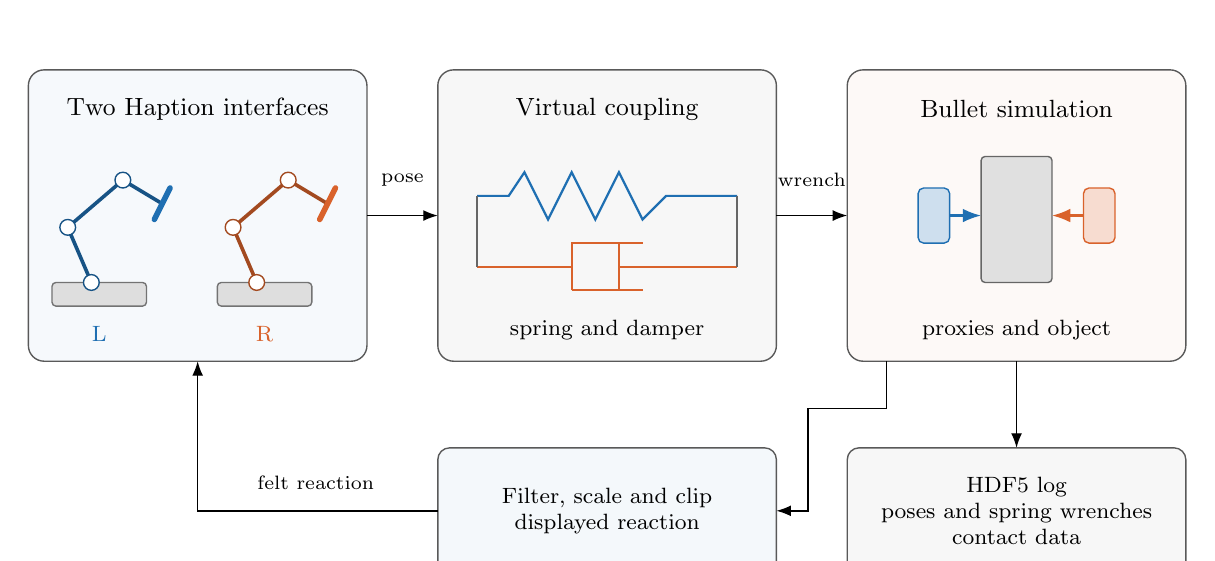
\begin{tikzpicture}[x=1mm,y=1mm,>=Latex,font=\small,line width=0.5pt]
\definecolor{haptionleft}{HTML}{1F6FB2}
\definecolor{haptionright}{HTML}{D9622B}
% Three compact panels: devices, numerical coupling and simulated bodies.
\draw[rounded corners=2mm,fill=haptionleft!4,draw=black!65] (0,0) rectangle (43,37);
\draw[rounded corners=2mm,fill=black!3,draw=black!65] (52,0) rectangle (95,37);
\draw[rounded corners=2mm,fill=haptionright!4,draw=black!65] (104,0) rectangle (147,37);
\node at (21.5,32) {Two Haption interfaces};
\node at (73.5,32) {Virtual coupling};
\node at (125.5,32) {Bullet simulation};
% Stylised articulated devices; these are explanatory silhouettes, not CAD.
\foreach \x/\col/\side in {0/haptionleft/L,21/haptionright/R}{
  \begin{scope}[shift={(\x,0)}]
  \draw[fill=black!13,draw=black!55,rounded corners=0.5mm] (3,7) rectangle (15,10);
  \draw[draw=\col!75!black,line width=1.3pt,line cap=round,line join=round]
    (8,10)--(5,17)--(12,23)--(17,20);
  \foreach \p in {(8,10),(5,17),(12,23)}
    \filldraw[fill=white,draw=\col!75!black] \p circle (1mm);
  \draw[draw=\col,line width=2pt,line cap=round] (16,18)--(18,22);
  \node[text=\col,font=\footnotesize] at (9,3.5) {\side};
  \end{scope}
}
% Spring and damper icon, standing for the two six-axis coupling channels.
\draw[draw=haptionleft,line width=0.8pt]
  (57,21)--(61,21)--(63,24)--(66,18)--(69,24)--(72,18)--(75,24)--(78,18)--(81,21)--(90,21);
\draw[draw=haptionright,line width=0.8pt] (57,12)--(69,12);
\draw[draw=haptionright,line width=0.8pt] (69,9)--(69,15)--(78,15) (69,9)--(78,9);
\draw[draw=haptionright,line width=0.8pt] (75,9)--(75,15) (75,12)--(90,12);
\draw[draw=black!60] (57,12)--(57,21) (90,12)--(90,21);
\node[font=\footnotesize] at (73.5,4) {spring and damper};
% Two opposing proxies and the body they touch.
\draw[fill=black!12,draw=black!60,rounded corners=0.5mm] (121,10) rectangle (130,26);
\draw[fill=haptionleft!22,draw=haptionleft,rounded corners=0.7mm] (113,15) rectangle (117,22);
\draw[fill=haptionright!22,draw=haptionright,rounded corners=0.7mm] (134,15) rectangle (138,22);
\draw[->,draw=haptionleft,line width=0.8pt] (117,18.5)--(121,18.5);
\draw[->,draw=haptionright,line width=0.8pt] (134,18.5)--(130,18.5);
\node[font=\footnotesize] at (125.5,4) {proxies and object};
\draw[->] (43,18.5)--(52,18.5);
\node[font=\scriptsize] at (47.5,23) {pose};
\draw[->] (95,18.5)--(104,18.5);
\node[font=\scriptsize] at (99.5,23) {wrench};
% Rendered feedback and logging are distinct branches.
\draw[rounded corners=1.5mm,fill=haptionleft!5,draw=black!65] (52,-27) rectangle (95,-11);
\node[align=center,font=\footnotesize] at (73.5,-19) {Filter, scale and clip\\displayed reaction};
\draw[rounded corners=1.5mm,fill=black!3,draw=black!65] (104,-27) rectangle (147,-11);
\node[align=center,font=\footnotesize] at (125.5,-19) {HDF5 log\\poses and spring wrenches\\contact data};
\draw[->] (125.5,0)--(125.5,-11);
\draw[->] (109,0)--(109,-6)--(99,-6)--(99,-19)--(95,-19);
\draw[->] (52,-19)--(21.5,-19)--(21.5,0);
\node[font=\scriptsize] at (36.5,-15.5) {felt reaction};
\end{tikzpicture}
\caption{Recording architecture, with schematic device silhouettes. The left and right interfaces are blue and orange, as in the wrench plots. Mapped device poses set the targets of numerical spring--damper couplings; these drive the simulated proxies against the object. The operator receives a filtered, scaled and clipped reaction. The log retains the spring-wrench signals and contact data separately from that displayed feedback.}
\label{fig:recording}
\end{figure}

\section{Position mapping and mirrored hands}

Let $\vect p_{H,h}(t)$ be the device position for hand $h$, and let the initial calibrated position be $\vect p_{H,h}(0)$. The target is
\begin{equation}
\vect p_{t,h}(t)=\vect p_{0,h}+R_{H\rightarrow W}
\bigl(\vect p_{H,h}(t)-\vect p_{H,h}(0)\bigr),
\qquad
R_{H\rightarrow W}=\begin{bmatrix}0&1&0\\-1&0&0\\0&0&1\end{bmatrix}.
\label{eq:haptic-map}
\end{equation}
The constant rotation aligns the workspace directions. Separate baseline orientations make the tools face each other. A bilateral setup cannot be treated as two copies of one local frame: a positive local push on each tool must correspond to opposite world directions.

For rotations, device increments are conjugated by the same frame rotation and composed with the hand baseline. Feedback vectors are mapped back with $R_{H\rightarrow W}^\top$. Because this map is a proper rotation, it preserves vector lengths and cross products. The later statistical right-hand convention is also a proper $180^\circ$ rotation; it must not be confused with a reflection of only one axis.

\section{Virtual coupling}

Figure~\ref{fig:virtual-coupling-schematic} shows one translational channel. The mapped handle target and the simulated proxy can have different poses; their displacement produces the elastic part of the interaction.

For a proxy at $\vect p_h$ with velocity $\vect v_h$, the translational command is
\begin{equation}
\vect F_{\mathrm{cmd},h}=K_p(\vect p_{t,h}-\vect p_h)-K_d\vect v_h-m_h\vect g.
\label{eq:translation-coupling}
\end{equation}
Here $\vect g$ points downward, so $-m_h\vect g$ compensates the proxy's own weight. This compensation is unrelated to estimating the manipulated object's unknown mass.

\begin{figure}[htbp]\centering
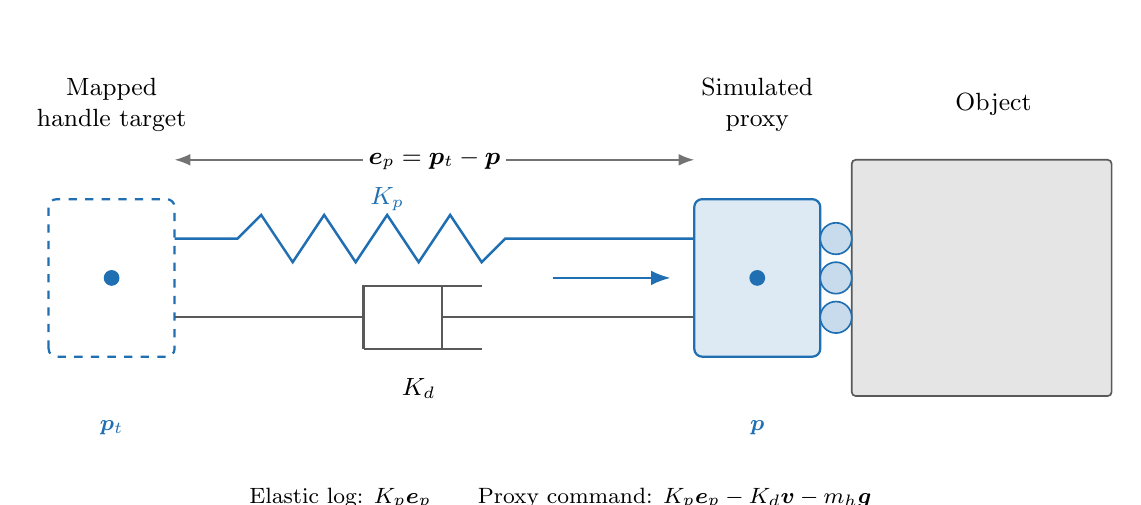
\begin{tikzpicture}[x=1mm,y=1mm,>=Latex,font=\small,line width=0.6pt]
\definecolor{haptionleft}{HTML}{1F6FB2}
% Mapped target is an outline; the proxy is the simulated physical body.
\node[align=center] at (16,44) {Mapped\\handle target};
\node[align=center] at (98,44) {Simulated\\proxy};
\node at (128,44) {Object};
\draw[dashed,draw=haptionleft,line width=0.8pt,rounded corners=1mm] (8,12) rectangle (24,32);
\draw[fill=haptionleft!15,draw=haptionleft,line width=0.8pt,rounded corners=1mm] (90,12) rectangle (106,32);
\fill[haptionleft] (16,22) circle (1mm);
\fill[haptionleft] (98,22) circle (1mm);
\draw[fill=black!10,draw=black!65,rounded corners=0.5mm] (110,7) rectangle (143,37);
\foreach \y in {17,22,27}{\filldraw[fill=haptionleft!25,draw=haptionleft] (108,\y) circle (2mm);}
% Parallel elastic and damping paths, shown only for translation.
\draw[draw=haptionleft,line width=0.9pt]
  (24,27)--(32,27)--(35,30)--(39,24)--(43,30)--(47,24)--(51,30)--(55,24)--(59,30)--(63,24)--(66,27)--(90,27);
\node[fill=white,inner sep=1pt,text=haptionleft] at (51,32) {$K_p$};
\draw[draw=black!65,line width=0.8pt] (24,17)--(48,17);
\draw[draw=black!65,line width=0.8pt] (48,13)--(48,21)--(63,21) (48,13)--(63,13);
\draw[draw=black!65,line width=0.8pt] (58,13)--(58,21) (58,17)--(90,17);
\node[fill=white,inner sep=1pt] at (55,8) {$K_d$};
\draw[<->,draw=black!55] (24,37)--node[fill=white,inner sep=2pt] {$\vect e_p=\vect p_t-\vect p$}(90,37);
\node[font=\footnotesize,text=haptionleft] at (16,3) {$\vect p_t$};
\node[font=\footnotesize,text=haptionleft] at (98,3) {$\vect p$};
\draw[->,draw=haptionleft,line width=0.9pt] (72,22)--(87,22);
\node[align=center,font=\footnotesize] at (73,-6) {Elastic log: $K_p\vect e_p$\qquad Proxy command: $K_p\vect e_p-K_d\vect v-m_h\vect g$};
\end{tikzpicture}
\caption{One translational virtual-coupling channel. The dashed target is obtained from the handle pose; the solid proxy moves under simulated dynamics and contact. The spring is numerical, not a physical spring mounted on the Haption. Damping uses proxy velocity, and gravity compensation is added to the proxy command. Only the elastic component is stored in the spring-wrench log. Rotation has the analogous stiffness--damping channel; the right hand uses the same structure.}
\label{fig:virtual-coupling-schematic}
\end{figure}

The rotational error is represented by the relative quaternion
\begin{equation}
q_e=q_t\otimes q_h^{-1}.
\end{equation}
The implementation extracts its axis and shortest rotation angle, setting the rotation vector to zero near the identity. If $\vect e_R=\theta\vect a$ denotes that vector, the command moment is
\begin{equation}
\vect \tau_{\mathrm{cmd},h}=K_{p,R}\vect e_R-K_{d,R}\vect\omega_h.
\label{eq:rotation-coupling}
\end{equation}
Quaternion coordinates avoid Euler-angle singularities, but the shortest-axis convention remains ambiguous at exactly $180^\circ$. The recorded operating range does not justify describing the orientation controller as globally nonsingular.

The source inspected for Experiment 13 uses $K_p=1500$ N/m and $K_{p,R}=40$ Nm/rad. These are gains of the virtual coupling, not stiffness measurements of a human arm. The translation and rotation channels have different units. A characteristic length $d$ relates their stiffness scales through $K_{p,R}=K_p d^2$; for these values, $d\simeq0.163$ m.

\section{What the wrench log contains}

The datasets \sourcefile{wrench_L} and \sourcefile{wrench_R} contain the elastic spring components, $K_p\vect e_p$ and $K_{p,R}\vect e_R$. The C++ command also contains damping and gravity compensation. Consequently, the logged wrench is a proxy for the transmitted quasi-static load, not an exact direct contact-wrench measurement at every instant.

For a settled proxy, acceleration and damping become small and the spring reaction can approximate the external contact load. During rapid movement, the equality no longer follows. This is why the recording protocol and later sample selection must restrict motion and check residuals. A high sampling frequency cannot itself make a trajectory quasi-static.

Direct contact data provide a complementary measurement. Each pad supplies a normal magnitude, two lateral-friction magnitudes and their directions. Their vector sum reconstructs the force on the selected body, with the sign determined by the body ordering. Summing moment arms reconstructs a wrench about a chosen pole. Comparing this contact wrench with the coupling wrench is a measurement check; replacing one silently with the other would change what the model learns.

\section{Filtering, display scale and saturation}

The feedback uses an exponential filter,
\begin{equation}
\bar{\vect F}_k=\alpha\vect F_k+(1-\alpha)\bar{\vect F}_{k-1},
\qquad \alpha=0.15,
\end{equation}
with the analogous expression for moment. The displayed wrench is then scaled and clipped to device limits. The session-C metadata report force and moment scales of $0.25$, a displayed-force limit of $20$ N and a displayed-moment limit of $2$ Nm. The corresponding pre-scale thresholds are $80$ N and $8$ Nm.

Equal force and moment scales preserve the geometric ratio associated with a moment arm while neither channel is saturated. More precisely, if $\vect\tau=\vect r\times\vect F$, the observable perpendicular offset is
\begin{equation}
\vect r_\perp=\frac{\vect F\times\vect\tau}{\norm{\vect F}^2}.
\end{equation}
Scaling force by $a_F$ and moment by $a_T$ multiplies this offset by $a_T/a_F$. This is a geometric property of the displayed signal. It does not prove that the operator's perceived CoM equals the physical CoM, especially after filtering, clipping or contact slip.

\section{Protocol and file structure}

The standardized recording divides the task into timed phases: grasp from $0$ to $7$ s, lift from $7$ to $15$ s, wielding from $15$ to $37$ s, and replacement from $37$ to $44$ s, followed by the final phase. The phase labels are stored explicitly. Learning can select a phase without inferring it from a force threshold whose behaviour changes with object mass.

\begin{table}[htbp]\centering\small
\begin{tabular}{@{}lp{0.60\textwidth}@{}}\toprule
Signal group & Purpose \\\midrule
Time and phase & Synchronization and separation of manipulation phases.\\
Hand and object poses & Frame transforms, tilt coverage and relative drift.\\
Left and right spring wrenches & Twelve-dimensional coordination signal.\\
Velocities & Checks on motion and quasi-static validity.\\
Pad contact records & Contact availability and friction-force reconstruction.\\
Gain, scale and limit metadata & Identification of the recording apparatus.\\
True simulated CoM and mass & Construction and retrospective error reporting.\\
Perturbation metadata & Separation of unperturbed and disturbed trials.\\
\bottomrule\end{tabular}
\caption{Roles of the HDF5 data groups. The presence of ground truth in a log does not authorize its use in autonomous decisions.}
\label{tab:hdf5}
\end{table}

Unperturbed demonstrations and disturbance trials answer different questions. A person resisting an injected torque is not simply performing the same natural wielding task with more samples. The prior training therefore excludes perturbed trials according to their recorded metadata.

\section{Why the rotational channel changed}

The earlier rotational coupling used $0.5$ Nm/rad. A $0.2$ Nm spring moment requires $0.4$ rad, approximately $23^\circ$, of angular lag at that stiffness. At $40$ Nm/rad, the same spring moment requires $0.005$ rad, approximately $0.29^\circ$. This calculation explains why a low-gain proxy can change orientation substantially instead of transmitting the intended torsional signal.

The measurements in Chapter~\ref{ch:evidence} show the resulting trade-off. The compliant recording retained nearly all pads, but only about $22\%$ of the reference moment was transmitted. The torsional covariance therefore cannot be interpreted as a property of human coordination alone. Raising rotational stiffness was a correction to the measurement apparatus, with a cost in surface conformity that later motivates the passive tool.

The valid prior uses session C, runs 024--036, at $K_{p,R}=40$ Nm/rad. A missing model file is treated as an error. Substituting the earlier model would change the apparatus represented by the prior without changing the controller configuration.

\section{Recording limitations}

The demonstrations come from a limited recording population and a standardized object. Their coverage is not a complete sphere of gravity directions. The useful empirical support is approximately $55^\circ$ of tilt for the final prior. A numerical GMR output outside that range is an extrapolation, even if its covariance remains finite.

The acquisition loop records many samples per run, but neighbouring samples share the same movement and contact history. They are not independent experimental repetitions. Statistical comparisons should retain run-level structure. The purpose of the dataset is to construct an apparatus-specific coordination prior and to test its transmission properties, not to establish a population-wide law of human manipulation.


\chapter{Contact Model and End-Effector Evolution}
\label{ch:contacts}

The contact model determines which moments the hands can transmit. The end-effector mechanism determines whether the assumed contacts can be maintained. The two must be described together. A mathematically admissible wrench at three nominal points is not useful if only one point reaches the object or if an unmodelled plate carries part of the load.

\section{Why one point is insufficient}

A point contact with friction supplies a three-dimensional force. It has no independent local moment. For two opposing point contacts, rotation about the line joining them cannot be resisted by assigning a torsional moment at either point. The limitation is geometric, not a shortcoming of the friction inequality.

To see this, let the two contact locations be $\vect p_1=\vect c-a\vect e_x$ and $\vect p_2=\vect c+a\vect e_x$. The component of their resultant moment along $\vect e_x$ is
\begin{equation}
\vect e_x^\top\bigl((-a\vect e_x)\times\vect f_1
+(a\vect e_x)\times\vect f_2\bigr)=0.
\end{equation}
No choice of the two point forces creates a moment about that axis. A stronger squeeze at the same two positions cannot remove this null direction.

\section{Exactly three discrete contacts per hand}

Each tool places three spherical contact elements at the vertices of a planar triangle. In the current tool coordinates, the push axis is $x$, the pad plane is $x=d$, and the locations are
\begin{equation}
\vect c_1=\begin{bmatrix}d\\0\\r\end{bmatrix},\quad
\vect c_2=\begin{bmatrix}d\\\sqrt{3}r/2\\-r/2\end{bmatrix},\quad
\vect c_3=\begin{bmatrix}d\\-\sqrt{3}r/2\\-r/2\end{bmatrix}.
\label{eq:pad-geometry}
\end{equation}
The inspected implementation uses $d=20$ mm, $r=30$ mm and sphere radius $10$ mm. Earlier device conventions used a different local pushing axis. Coordinates must be transformed explicitly rather than merged by reusing axis names.

\begin{figure}[htbp]\centering
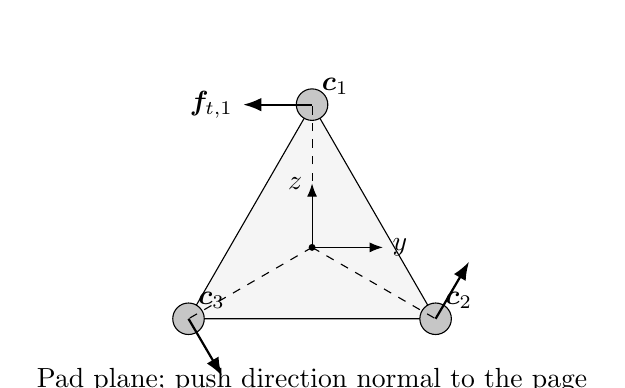
\begin{tikzpicture}[scale=1.25,>=Latex]
\coordinate (a) at (0,1.45);\coordinate (b) at (1.255,-0.725);\coordinate (c) at (-1.255,-0.725);
\draw[fill=gray!8] (a)--(b)--(c)--cycle;
\foreach \pt/\lab in {a/1,b/2,c/3}{\draw[fill=gray!45] (\pt) circle (0.16);\node[above right] at (\pt) {$\vect c_{\lab}$};\draw[dashed] (0,0)--(\pt);}
\fill (0,0) circle (1pt);\draw[->] (0,0)--(0.72,0) node[right] {$y$};\draw[->] (0,0)--(0,0.65) node[left] {$z$};
\node at (0,-1.35) {Pad plane; push direction normal to the page};
\draw[->,thick] (a)--++(-0.7,0) node[left] {$\vect f_{t,1}$};
\draw[->,thick] (b)--++(0.34,0.58);\draw[->,thick] (c)--++(0.34,-0.58);
\end{tikzpicture}
\caption{Three discrete contact points. Tangential forces act at nonzero lever arms and create torsion about the push axis. No local torsional moment is assigned to a point.}
\label{fig:tripad-geometry}
\end{figure}

The spheres are geometric contact elements. Their use does not turn the model into a soft-finger contact or a continuous friction patch. In the allocator, each sphere contributes one resultant point force, and each hand always has three possible force slots. A slot is set to zero when its pad is inactive.

\section{Wrench aggregation and torsional capacity}

About a wrist position $\vect b_h$, the hand wrench is
\begin{equation}
\vect F_h=\sum_{i=1}^3\vect f_{hi},\qquad
\vect\tau_h=\sum_{i=1}^3(\vect p_{hi}-\vect b_h)\times\vect f_{hi}.
\label{eq:hand-wrench}
\end{equation}
For a planar triangle centred on the push axis, the axial moment is
\begin{equation}
\tau_x=\sum_{i=1}^3(y_i f_{z,i}-z_i f_{y,i}).
\end{equation}
It emerges from tangential force components. The same components may also be needed to support weight, so maximum torsion and maximum vertical load cannot be demanded independently.

If all three contacts have radius $r$, parallel normals and compressive magnitudes $\lambda_i$, Coulomb friction gives the upper bound
\begin{equation}
|\tau_x|\leq \sum_i r\norm{\vect f_{t,i}}
\leq\mu r\sum_i\lambda_i.
\label{eq:torsion-bound}
\end{equation}
For a symmetric pure-torsion allocation, the bound can be attained by circulating tangential forces whose resultant cancels. It is generally only a bound in a loaded grasp. Gravity, unequal contact loads and nonparallel normals consume the same friction capacity. The allocator resolves that coupling directly.

\section{Contact measurements from Bullet}

A contact record contains a normal-force magnitude $f_n$, two lateral magnitudes $f_1,f_2$ and their directions $\vect d_1,\vect d_2$. After choosing the correct body sign, its vector is reconstructed as
\begin{equation}
\vect f=f_n\vect n_c+f_1\vect d_1+f_2\vect d_2.
\label{eq:bullet-contact}
\end{equation}
The C++ acquisition uses the fields \sourcefile{m_normalForce} and \sourcefile{m_linearFrictionForce1/2} of \sourcefile{b3ContactPointData}. Contact positions provide the moment arms. Explicit reconstruction permits force-balance checks and visualization of the actual tangential components.

The Python tool reads the corresponding exposed contact records and groups them by sphere link. A pad may have more than one manifold entry even though the optimization has one force variable for that pad. The reduction to one position, normal and resultant per pad is therefore part of the measurement model. It should be checked on edges where normals vary, rather than assumed harmless because the tool has three spheres.

\section{Rigid tri-pad and compliant wrist}

The first triangular tool fixes the three pads to the flange. Misalignment is accommodated by the wrist virtual coupling. For a small tilt with moment $M$, the rotational deflection is approximately $\theta=M/k_{\mathrm{tilt}}$. If a squeeze $F$ acts through an effective lever of order $r$, then
\begin{equation}
\theta\simeq\frac{Fr}{k_{\mathrm{tilt}}}.
\label{eq:force-tilt}
\end{equation}
This is a local explanatory relation, not a calibrated global law. It shows why increasing force can change geometry. A displaced wrist changes the opposition of the contacts, the optimizer sees a less favourable grasp, and a fallback that increases squeeze can amplify the original deflection.

The documented force ladder in Chapter~\ref{ch:evidence} demonstrates the consequence on one object: a high squeeze fails earlier than a lower one. The result does not identify a universal optimal force. It rejects the assumption that the force setting can be increased independently of the geometry.

\section{Axial pad travel}

The next design gives each pad an axial travel coordinate. Peripheral springs permit differential movement, while a central contribution supports the common push mode. For a symmetric small-displacement model,
\begin{equation}
k_{\mathrm{ax}}=3k+K_c,\qquad
k_{\mathrm{tilt}}=\frac32kr^2.
\label{eq:rail-stiffness}
\end{equation}
The central spring acts at the triangle centre, so it does not contribute a tilt moment about that centre. This permits axial stiffness to increase without imposing the same increase on surface-conforming tilt.

With axial-only pad springs, rotation about the push axis does not deform those springs. Their axial model contributes no torsional spring stiffness. Torsional resistance at the object still comes from the discrete contact forces. Lateral constraints of a prismatic joint are mechanical constraints; they must not be interpreted as learned human stiffness.

Finite travel limits conformity. With $r=30$ mm and travel $8$ mm, a simple one-pad differential displacement corresponds to an angle of approximately $\arcsin(8/30)=15.5^\circ$. At a travel stop the tool changes behaviour. Reporting spring stiffness without reporting travel would omit the condition under which the mechanism becomes effectively rigid.

\section{Floating triangular plate}

The later tool joins the three spheres to one rigid triangular plate. Peripheral springs connect flange supports to the sphere centres, and a central six-degree-of-freedom spring connects the flange to the plate centre. Both spring sets act between the same two rigid bodies and therefore contribute in parallel. The wrist coupling is upstream of this tool; its compliance combines in series only in an uncoupled channel approximation.

Let $\vect\xi=(\vect d,\vect\phi)$ be a small displacement of the plate. At attachment $\vect a_i$, measured from the plate centre,
\begin{equation}
\Delta_i\simeq B_i\vect\xi,\qquad
B_i=\begin{bmatrix}I&-\crossmat{\vect a_i}\end{bmatrix}.
\end{equation}
For peripheral stiffness matrices $K_i$ and central stiffness $K_c^{(6)}$,
\begin{equation}
U\simeq\frac12\vect\xi^\top K_{\mathrm{tool}}\vect\xi,
\quad
K_{\mathrm{tool}}=K_c^{(6)}+\sum_i B_i^\top K_iB_i.
\label{eq:tool-stiffness}
\end{equation}
This is the small-rotation Hessian used by the stiffness scripts. Zero-free-length springs give quadratic energy in attachment displacement~\cite{herder2001}; the mapping from a finite rotation to attachment displacement is still nonlinear. Stability conclusions from Equation~\eqref{eq:tool-stiffness} are local and limited to the modelled free directions~\cite{guest2006}.

The inspected floating-plate defaults use $500$ N/m in the peripheral axial and lateral directions, $20000$ N/m central translational stiffness, $40$ Nm/rad central torsion and zero central tilt stiffness. The symmetric local model gives
\begin{equation}
k_{\mathrm{ax}}=21500\ \mathrm{N/m},\quad
k_{\mathrm{tilt}}=0.675\ \mathrm{Nm/rad},\quad
k_{\mathrm{tors}}=41.35\ \mathrm{Nm/rad}.
\end{equation}
The last value includes $3k_{\mathrm{lat}}r^2=1.35$ Nm/rad from the peripheral lateral springs. It would be incorrect to transfer the zero torsional stiffness of the axial rail design to this plate design.

The plate's torsional mounting stiffness does not add a soft-finger moment at the object. It transmits the moment generated by the three contact forces from the plate to the wrist. Keeping these two levels distinct preserves the discrete-point model.

\section{Compliance centre and transmission}

In the symmetric arrangement, $\sum_i\vect a_i=0$, and the translation--rotation coupling block vanishes at the plate centre. More generally, the compliance centre follows the stiffness-weighted attachment geometry. This connects the design to the remote-centre-compliance reasoning of Whitney~\cite{whitney1982}.

If the full stiffness matrix contains coupling, a channel's effective stiffness under free motion of the other coordinates is obtained from the compliance $C=K^{-1}$, as $1/C_{jj}$. Reading $K_{jj}$ gives the stiffness when the other coordinates are held fixed. The two measurements need not agree. The floating-plate code explicitly uses the compliance interpretation.

The wrist and tool form two deformable stages. For an independent channel with stiffnesses $k_w$ and $k_t$, the combined stiffness is
\begin{equation}
k_{\mathrm{eq}}=\left(k_w^{-1}+k_t^{-1}\right)^{-1}.
\end{equation}
This relation cannot be applied by adding peripheral and central stiffness reciprocals: those springs are parallel, not series. For coupled six-dimensional mechanics, the appropriate quantities are compliance matrices expressed about the same pole.

\section{Unmodelled plate contacts}

A plate collision can introduce a load path outside the three sphere links. The floating-plate module gives the plate a collision shape by default; the geometry campaign of Chapter~\ref{ch:geometry} turns it off and runs the colliding plate only as a declared ablation. The flange carries no collision shape at all, so it cannot touch the object. A recorded pilot case with a plate contact rejected all estimation samples because the measured sphere-force resultant no longer matched the supported load.

This is a model-completeness problem. Counting three optimized pads does not make an additional physical plate contact disappear. To preserve the intended experiment, the plate must either remain clear of the object or the run must be identified as violating the six-point model. Adding a hidden support force to the estimator would conceal the issue.

The geometry campaign therefore records, on every control tick, every contact between the object and any tool part that is not one of the six spheres, with the normal force it carries. Table~\ref{tab:plate-collision} compares the same 182 bodies with the plate visual only and with the plate colliding; nothing else changes, and neither arm uses the wrist re-alignment controller.

\begin{table}[htbp]\centering\small
\begin{tabular}{@{}lrr@{}}\toprule
 & Visual-only plate & Colliding plate\\
\midrule
Bodies on which the plate touched the object & 0 / 182 & 74 / 182\\
\quad of which jittered cubes / polytopes & 0 / 0 & 5 / 69 (of 96 / 80)\\
Largest load carried by the plate & 0 N & 142.5 N\\
Share of the squeeze through the plate (touching runs, median / max) & -- & 0.39 / 0.92\\
Polytopes: estimator abstentions & 5 & 59\\
Polytopes: estimation samples rejected (median) & 0\% & 98\%\\
Polytopes: SOCP allocations accepted & 0.985 & 0.768\\
Polytopes: realized wrench error (median) & 4.0 N & 30.1 N\\
Polytopes: bodies placed & 63 & 61\\
\bottomrule\end{tabular}
\caption{Load-path audit of the floating plate on the geometry campaign. A colliding plate touches 69 of 80 random polytopes, carries up to 92\% of the squeeze, and breaks the estimate on most of them, while the number of bodies placed hardly changes.}
\label{tab:plate-collision}
\end{table}

The last row is the point. A plate that carries part of the load places almost as many bodies as a clean one, so the visible outcome does not reveal the violation; the measurement does. The wrench the contacts actually apply misses the allocated one by 30 N instead of 4 N, and the estimator, which assumes every newton comes through the spheres, rejects most of its samples. A second observation concerns control rather than geometry: in an earlier launch of the same campaign with the wrist re-alignment controller active, the colliding plate touched 47 of the 96 jittered cubes, against 5 of 96 without it. Re-commanding the wrist tilts the plate into the object. The thesis comparison uses the visual-only plate and no re-alignment.

The end-effector evolution therefore follows one requirement: conform to uncertain surfaces while preserving a measurable, finite load path. The rigid tool, axial-travel tool and floating plate are different implementations of that requirement and must be evaluated as separate apparatus configurations.


\chapter{Human Coordination and the Orientation-Dependent Prior}
\label{ch:prior}

Two hands can redistribute a load while leaving the object's resultant wrench unchanged. Demonstrations record how that redistribution occurs. This chapter explains the interpretation of their variability and how it enters the controller. The statistical method is established; the adaptations concern wrench coordinates, changing attitude and the recording apparatus.

\section{Task-equivalent variations and UCM}
\label{sec:ucm-prior}

The uncontrolled manifold (UCM) approach distinguishes variations that preserve a selected task variable from variations that change it~\cite{scholz1999}. Here the task variable is the resultant object wrench, and the elemental variables are the two wrist wrenches:
\begin{equation}
\vect w=\begin{bmatrix}\vect F_L\\\vect\tau_L\\\vect F_R\\\vect\tau_R\end{bmatrix}\in\R^{12}.
\label{eq:wrench12}
\end{equation}
At fixed hand positions, shifting both wrist moments to a common object pole and summing gives a linear map $G_w$. A redistribution is task-equivalent when
\begin{equation}
G_w\Delta\vect w=\vect0.
\label{eq:ucm-wrench}
\end{equation}
This null space is the local UCM for the chosen task. An equal increase in opposing squeeze forces is a simple example: it adds no resultant object force, although the hands work harder. Task equivalence does not ensure admissibility under friction or actuator limits.

UCM analysis compares variance within this subspace with variance in directions that change the task, normalized by their dimensions. Force and moment coordinates require an explicit scaling. Campolo et al. show why geometric metrics matter in UCM analysis~\cite{campolo2013}; their pointing task differs from this wrench task.

\thesisfigure{ch05_prior/ucm_session_c.pdf}{Bimanual coupling in session C ($K_{p,\mathrm{rot}}=40$, 13 runs, residuals per run and gravity cell). Left: moment about the grasp axis, left hand against right; the cloud lies along the internal direction, which leaves the sum of the two hand moments unchanged (the moments of the hand forces about the CoM are not included in this panel). Right: the index $r=1-2\,n^\top\Sigma_{LR}n/(n^\top\Sigma_{LL}n+n^\top\Sigma_{RR}n)$ on the grasp triad, $1$ for independent hands, above $1$ when variability goes into the internal mode. Bars show 95\% bootstrap intervals over runs; grey marks an interval that contains $1$. Force indices near $2$ are imposed by quasi-static equilibrium; the moment channel carries the information.}{fig:ucm-session-c}

The index is computed per direction on residuals conditioned on the gravity direction; it is not the full spatial variance ratio of the classical method. An earlier whole-space analysis of the project compared each mode with a surrogate that shuffled every coordinate independently; that surrogate also destroyed the correlation within each hand, and the analysis is not used here. These analyses describe recorded coordination; mechanics can structure covariance too, so they do not establish a neural origin~\cite{valero2009,kutch2012}.

\section{From covariance to precision}

UCM and precision are related, but different. UCM identifies task-preserving directions from a task map. Covariance $\Sigma_w$ describes the observed wrench distribution. Its regularized inverse is the \emph{precision matrix}:
\begin{equation}
Q_w=\Sigma_w^{-1},\qquad
J_{\mathrm{prior}}=\tfrac12(\vect w-\vect\mu_w)^\top Q_w(\vect w-\vect\mu_w).
\label{eq:prior-mahalanobis}
\end{equation}
This is the quadratic part of a Gaussian negative log-likelihood, or a squared Mahalanobis penalty~\cite{bishop2006}. Large demonstrated variance gives a small penalty; little variance gives a larger penalty. Cross-hand covariance retains coordinated departures instead of treating the hands independently.

The intended preference is to permit common demonstrated variations and discourage departures from tightly maintained patterns. A broad covariance direction need not coincide exactly with the UCM. The controller uses the full conditional precision: it does not project its decision onto a learned manifold or put the scalar UCM index in the cost. Contact constraints separately define feasibility.

The active allocator of Chapter~\ref{ch:socp} uses the precision without the mean, $J=\vect w^\top W(R)\vect w$, and imposes equilibrium exactly. The task component of $\vect w$ is then fixed by the constraints, and the cost only ranks the internal wrenches, those that satisfy Equation~\eqref{eq:ucm-wrench}. The precision is therefore used on the subspace that the UCM decomposition calls task-equivalent: directions in which the demonstrations varied are cheap, directions they kept tight are expensive. The mean-centred form of Equation~\eqref{eq:prior-mahalanobis} belongs to the previous allocator (Section~\ref{sec:socp-previous}).

A recording interface that suppresses torsion can create narrow covariance and an excessive torsional penalty. The valid prior therefore comes from high-stiffness session C. Better apparent seating under soft rotational coupling is insufficient if the moment to be learned is attenuated.

\section{Static lift and changing orientation}

A conventional GMM can describe a selected upright lift phase, giving a constant precision. Wielding changes gravity direction in object coordinates, so the expected wrench and covariance must vary with attitude.

Calinon's task-parameterized GMM and Gaussian mixture regression provide this adaptation~\cite{calinon2016}. Demonstrations are encoded in world and box frames. At the current attitude, their transformed Gaussian models are combined and conditioned on local gravity, returning $\vect\mu_w(\hat{\vect g}_{\mathrm{local}})$ and $Q_w(\hat{\vect g}_{\mathrm{local}})$. The general fitting and regression derivations are left to the cited method.

The final training selects the wielding phase and uses five mixture components. These are components within one phase, not five identified task stages. The following details explain the implementation choices needed for wrench data.

\section{Hand convention, units and frame adaptation}

The right-hand force and moment are transformed by the proper rotation $M=\diag(-1,-1,1)$ before training and transformed back at output. Both vectors use the same rotation. This aligns the opposing hand conventions without using a reflection.

Force and moment have different units. One scalar is used for every force axis and another for every moment axis:
\begin{equation}
S=\diag(s_F I_3,s_T I_3,s_F I_3,s_T I_3),\qquad
\tilde{\vect w}=S^{-1}\vect w.
\label{eq:scale12}
\end{equation}
The scalars come from pooled coordinate variances. Isotropic scaling within each vector commutes with rotation; axis-dependent scales would distort the task-frame transform.

The observation combines three unit-gravity coordinates and twelve scaled wrench coordinates. These five three-vectors rotate between frames. Wrist moments retain their wrist poles: rotating coordinates does not move the point about which a moment is measured.

At query time the world model rotates into box coordinates, while the box model is already there. The Gaussian product combines precision rather than averaging covariance. Regression conditions the mixture on local gravity. Its output covariance includes differences between conditional component means; otherwise ambiguous predictions would become artificially precise.

Fitting uses a $10^{-3}$ ridge in normalized coordinates, and the physical query adds a $10^{-5}$ numerical ridge before inversion. These are regularization choices, not measured noise variances. The query uses the learned mixture weights in regression. These details describe the implemented variant rather than new statistical results.

The solver evaluates the physical penalty in normalized coordinates using $Q_n=S^\top Q_wS$. This change of units preserves the quadratic form; Appendix~\ref{app:math} records the check. It does not change the physical preference.

\thesisfigure{ch05_prior/prior_query.pdf}{Queries of the saved session-C prior. Shaded outer ranges exceed the approximate $55^\circ$ empirical support and are extrapolations. These are model outputs, not measured control performance.}{fig:prior-query}

\section{Adapting the query to irregular bodies}

A generated polytope has an arbitrary mesh frame, which need not match the training box. The transfer defines a grasp frame at closure: $x$ follows the line between hands, $z$ is projected upward, and $y=z\times x$. It anchors that initial frame to the body:
\begin{equation}
R_{BG,0}=R_{WB,0}^\top R_{WG,0},\qquad
R_{WG}(t)=R_{WB}(t)R_{BG,0}.
\label{eq:anchored-grasp}
\end{equation}
Gravity is expressed in this moving frame. Rebuilding it from world vertical at every update would erase a roll about the grasp axis from the query.

This makes transfer well defined but does not prove that a box-trained distribution suits every shape. Its attitude coverage is limited and its absolute mean is tied to the demonstrated load. The current query does not automatically rescale the mean to a new estimated mass.

\section{Testing what the prior contributes}

The ablation below was run with the previous allocator of Section~\ref{sec:socp-previous}, which included the human mean and a contact-effort term; it has not been repeated with the active precision-only allocator. The full mode uses learned precision. The identity mode retains its mean and replaces precision with $(\operatorname{tr}Q_n/12)I$, removing directional preference while preserving total weight. The no-prior mode removes the term, leaving effort and equilibrium penalties. These are implemented ablations, not consequences of the UCM hypothesis.

Full versus identity tests demonstrated anisotropy. Full versus no prior tests the entire demonstrated preference. An unscaled identity would also change penalty strength and confound the comparison.

The comparison was run on the floating-plate tool over the 182 bodies of the geometry campaign (Chapter~\ref{ch:geometry}), with identical populations, friction, gates, trajectories and search seeds; only the prior mode changes. The bodies are held out by construction: the precision was learnt from virtual demonstrations on a standardised box, and none of these shapes was seen in training.

\begin{table}[htbp]\centering\small
\begin{tabular}{@{}lrrr@{}}\toprule
 & Full (TP-GMM) & Equal-trace identity & No prior\\
\midrule
Bodies placed, of 182 & 165 & 161 & 120\\
\quad one corner / jitter / polytopes & 6 / 96 / 63 & 6 / 96 / 59 & 6 / 85 / 29\\
Lost in the wielding & 15 & 15 & 51\\
Squeeze target, median & 43.5 N & 38.6 N & 23.4 N\\
Contact effort $\sum_i\norm{\vect f_i}^2$, measured, median & 1563 N$^2$ & 1472 N$^2$ & 479 N$^2$\\
Realized force error, median & 3.7 N & 3.5 N & 4.1 N\\
Realized moment error, median & 0.067 Nm & 0.061 Nm & 0.120 Nm\\
Estimator abstentions & 5 & 7 & 29\\
\bottomrule\end{tabular}
\caption{Prior ablation on the floating plate, same 182 bodies. Realized errors compare the wrench the contacts actually apply with the previous accepted allocation, about the same pole. Paired on the same body, full against identity: 12 bodies go further, 2 less, 168 the same ($p=0.013$), all of them polytopes; full against no prior: 50 further, 3 less ($p<0.001$).}
\label{tab:prior-ablation}
\end{table}

The two comparisons differ in size. Removing the prior term entirely lets the effort cost cut the squeeze by half and the contact effort by a factor of three, and objects drop in the wielding: 51 losses against 15, and nearly twice the moment error. Keeping the same total weight without the learnt shape, the identity arm, reproduces the full prior on all 102 cube-family bodies and falls slightly behind it on the 80 polytopes (59 placed against 63). On this apparatus most of the prior's contribution is therefore its \emph{weight} against the effort term; the demonstrated anisotropy adds a small but detectable benefit, and only where the contacts are most irregular. This last effect appeared only when the polytope population was doubled from ten to twenty bodies per band: at ten per band the same comparison gave 4 against 1 ($p=0.38$). Two limits apply: the contacts the allocator reads are exact in simulation, and only one prior model, session C, was tested.


\chapter{Inertial Estimation through Lift and Wielding}
\label{ch:estimation}

Estimation uses the load carried by the hands while the object is entirely in the air. A lift gives mass and two CoM components. Slow changes of orientation provide the third component. The estimator must also indicate when the accepted measurements do not support a three-dimensional answer.

\section{Why identify the load before reorientation?}

Wielding is active load identification before a requested orientation change. Two boxes can have equal mass and horizontal CoM coordinates but different CoM heights. Their upright gravity moments are identical; their moments after tilting need not be. An upright-only estimate can therefore support vertical transfer yet leave the later inclined allocation underdetermined.

This need is industrially relevant, although the present apparatus is not a deployed cell. Wong et al. demonstrate dual-arm lifting with online inertial estimation on real robots~\cite{wong2026}. Commercial payload identification also uses multiple diverse poses to estimate mass and CoM~\cite{urpayload}. These sources motivate identification; they do not validate this thesis's discrete-contact tool or prove a benefit from its human prior.

The appropriate downstream test is controlled reorientation under a changing gravity moment. Identification remains entirely airborne. Placement on an inclined fixture could be a later test, but support forces must never enter the free-space estimator. A ramp adds a release-stability problem and is not required to establish the value of the missing CoM coordinate.

\section{Equilibrium about a stated pole}

Let $\vect c$ be the reference pole and $\vect r_W=\vect p_{\mathrm{CoM}}-\vect c$. The total contact force and moment acting on the object satisfy
\begin{align}
\vect F_c+m\vect g&\simeq0,\\
\vect T_c(\vect c)+\vect r_W\times m\vect g&\simeq0.
\end{align}
Consequently,
\begin{equation}
\vect T_c(\vect c)\simeq m\vect g\times\vect r_W.
\label{eq:estimation-moment}
\end{equation}
The sign follows from the contact force acting on the object. A measured reaction on a hand has the opposite sign and must be converted before using this equation.

For a body-fixed pole, $\vect r_W=R_{WB}\vect r_B$. Define the first mass moment $\vect q=m\vect r_B$. Each accepted sample gives
\begin{equation}
\vect T_k=H_k\vect q+\vect e_k,\qquad
H_k=\crossmat{\vect g}R_{WB,k}.
\label{eq:regression}
\end{equation}
The equation is linear in $\vect q$. The pole must remain attached to the same body location, or its movement must be accounted for. Choosing a new arbitrary pole for every sample and keeping one $\vect r_B$ would make the regression inconsistent.

\section{Mass from the free-space resultant}

Under the same equilibrium assumption,
\begin{equation}
\hat m_k=\frac{\norm{\vect F_{c,k}}}{g_0},\qquad g_0=9.81\ \mathrm{m/s^2}.
\end{equation}
The current estimator uses the median of the recent twenty-five mass samples once enough samples are available. It estimates mass spread with the median absolute deviation multiplied by $1.4826$, with a floor of one per cent of the estimated mass. Before sufficient samples exist, it retains the declared mass prior.

The norm avoids sign ambiguity in the scalar mass, but it does not make nonvertical forces valid. External support, dragging or acceleration can change the resultant. The estimator therefore also checks its direction. In a free-space static hang, the contact resultant should oppose gravity.

\section{What a vertical lift observes}

At a constant attitude, $\crossmat{\vect g}R_{WB}$ has rank two. Its null vector is the body direction parallel to world gravity. At upright attitude,
\begin{equation}
\vect T_c=\begin{bmatrix}mg_0 r_y\\-mg_0 r_x\\0\end{bmatrix},\qquad
r_x=-\frac{T_y}{mg_0},\quad r_y=\frac{T_x}{mg_0}.
\label{eq:planar-estimate}
\end{equation}
The vertical coordinate is absent. Adding more upright samples cannot identify it. A minimum-norm solution may return zero for this coordinate, but zero is an algebraic convention rather than a measurement.

\thesisfigure{ch06_estimation/observability.pdf}{Singular values of the gravity-moment regressor for illustrative accepted attitudes. The upright data have rank two. Introducing a second nonparallel gravity direction removes the common null direction. This figure is an algebraic illustration, not an experimental convergence curve.}{fig:observability}

\section{Why wielding supplies the missing direction}

Stacking samples gives $H=(H_1^\top,\ldots,H_N^\top)^\top$. Its null space is the intersection of the individual null spaces. Two sufficiently different body-frame gravity directions have no common nonzero null vector, so full rank is possible.

The information matrix is
\begin{equation}
\mathcal I=\sum_k H_k^\top R_e^{-1}H_k,
\label{eq:information}
\end{equation}
for a stated moment-noise covariance $R_e$. If the noise is taken as isotropic and equal across samples, this is proportional to $H^\top H$. The smallest eigenvalue indicates the least informed parameter direction. This is the quasi-static counterpart of information-based trajectory design~\cite{wilson2014}.

A maximum tilt angle is insufficient evidence of observability. If only a few accepted samples occur at that angle while most are upright, the third singular value can remain small. The code records the gravity-direction swing over accepted samples and an observability ratio. The commanded trajectory is not substituted for the measured excitation.

Wielding is performed without a bottom pivot, table or wall. A support force would add an unknown wrench and change the regression. Rotations are slow movements of the dual-hand grasp, with pauses or sufficiently settled samples, rather than dynamic shaking intended to identify inertial tensors.

\section{The implemented least-squares estimator}

Earlier scripts use recursive least squares. The current passive-tool path instead retains accepted samples and solves an observed-subspace least-squares problem. Least squares is established~\cite[Section 3.1]{bishop2006}; the acceptance gates, rank threshold and uncertainty assigned to missing directions are implementation choices described below.

The current passive-tool estimator stores accepted regressors and moments and solves stacked least squares in the observable subspace. It diagonalizes
\begin{equation}
H^\top H=V\diag(\ell_1,\ell_2,\ell_3)V^\top.
\end{equation}
A direction is treated as observed if $\ell_j>\eta^2\ell_{\max}$ and exceeds a small absolute threshold; the default $\eta$ is $0.15$. The estimate is
\begin{equation}
\hat{\vect q}=\sum_{j\in\mathcal O}
\vect v_j\frac{\vect v_j^\top H^\top\vect T}{\ell_j},
\label{eq:subspace-estimator}
\end{equation}
where $\mathcal O$ contains only the observed directions.

This truncation prevents numerical noise in an almost-null direction from generating a large CoM component. It is not a way to declare that the omitted component is small. The omitted component remains unknown and receives prior variance.

\section{Uncertainty and unobserved coordinates}

Let the residual moment vector be $\vect e=\vect T-H\hat{\vect q}$. A residual variance estimate is
\begin{equation}
\hat\sigma_T^2=\frac{\vect e^\top\vect e}{\max(3N-|\mathcal O|,1)}.
\end{equation}
The first-moment covariance is constructed as
\begin{equation}
C_q=\sum_{j\in\mathcal O}\frac{\hat\sigma_T^2}{\ell_j}\vect v_j\vect v_j^\top
+\sum_{j\notin\mathcal O}(\hat m r_{\max})^2\vect v_j\vect v_j^\top.
\label{eq:cov-unobserved}
\end{equation}
The second term states the declared prior uncertainty in unobserved directions. A pseudoinverse alone would place zero covariance there, creating false confidence.

Since $\hat{\vect r}=\hat{\vect q}/\hat m$, first-order propagation gives
\begin{equation}
C_r\simeq \frac{C_q}{\hat m^2}
+\frac{\hat{\vect q}\hat{\vect q}^\top}{\hat m^4}\sigma_m^2.
\label{eq:mass-propagation}
\end{equation}
The code implements this expression without a cross-covariance between the mass and first-moment estimates. Both are computed from the same contact history, so independence is an approximation. The reported covariance also neglects uncertainty in orientation, normals and moment-pole position. It is a self-assessment under the regression model, not a calibrated confidence guarantee for all physical errors.

The code reports observed-subspace uncertainty separately from total covariance. During a static hang, total covariance is dominated by the unobserved direction. It cannot distinguish a good planar estimate from a poor one if only its trace is reported. A radius bound can clip an implausible CoM estimate; when clipping acts, it is recorded. The clipped result must not be presented as if all its coordinates were measured.

\section{Sample acceptance and abstention}

The estimator accepts samples only if the angular rate is below $0.30$ rad/s, the contact resultant exceeds $2$ N, at least four pads are present when contact count is supplied, and the resultant lies within $20^\circ$ of vertical. These are implemented checks, not a complete quasi-static certificate.

An angular-rate bound does not bound angular acceleration. Likewise, a vertical resultant can contain inertial load. The recording analysis therefore compares inertial terms with applied wrench where those signals are available. For a physical system, reliable acceleration or residual estimates would be needed to validate the same assumption.

The stage gate should use the estimator's own evidence: accepted sample count, observed directions, singular-value ratio, clipping, rejected-sample fraction and realized contact state. It must not inspect true CoM error. An estimate can abstain after a lift or after wielding if these conditions are inadequate. Every abstention remains in the campaign denominator.

\section{Using the estimate in control}

The estimated mass determines the gravity wrench. The estimated CoM determines the moment reference in the allocator. Both must use the same body-to-world pose estimate and the same stated pole. A good CoM estimate combined with a wrong pole still creates the wrong moment balance.

The uncertainty relevant to a particular pose can be examined through
\begin{equation}
C_{\tau}\simeq \hat m^2\crossmat{\vect g_B}C_r\crossmat{\vect g_B}^\top.
\end{equation}
An uncertain coordinate parallel to gravity creates no gravitational moment in that pose. On tilting, it can become load-bearing. This explains why the previously unobserved coordinate matters before the new orientation is reached. The equation is used here as an interpretation of estimation uncertainty; it is not added as a stochastic friction constraint.

\section{The inverse problem in the catalogue task}

For a catalogue tetromino, mass and CoM are known by declaration. The unknown becomes the grasp offset. A static hang supplies the two components perpendicular to gravity through the same moment balance. If the planned grasp centre is $\vect c_{\mathrm{plan}}$ and the measured CoM offset from the actual grasp pole is $\hat{\vect r}$, their relationship updates the believed object position relative to the hands.

The unobserved component is retained from the declared geometric plan, not set to a measured zero. Insertion depth is subsequently closed through seating feedback. This reuse of the regression is useful because the relevant unknown has changed, not because the catalogue task has somehow become a full blind CoM experiment.


\chapter{Convex Contact Force Allocation}
\label{ch:socp}

The allocator answers a local question: given the contacts available now and the load believed now, which wrench should each wrist apply to the object? Contact positions and normals are parameters during a solve. The human prior supplies the metric in which wrist wrenches are compared. Friction defines admissibility, and a signed friction margin keeps every planned contact force a fixed distance inside its cone.

This chapter presents the active formulation first: two wrist wrenches, twelve decision components, exact equilibrium and signed-distance friction margins. Section~\ref{sec:socp-previous} records the earlier eighteen-force formulation with slack, cap and a scaled cone. The population campaigns of Chapters~\ref{ch:geometry} and~\ref{ch:tetris} were run with that earlier allocator, so its equations and its audit remain part of the evidence.

\section{A short introduction to SOCP}

A second-order cone constraint has the form
\begin{equation}
\norm{A\vect x+\vect b}_2\leq\vect c^\top\vect x+d.
\end{equation}
Its feasible set is convex. Affine equalities, intersections of such cones and positive-semidefinite quadratic epigraphs remain convex~\cite{boyd2004}. A solver can therefore find a global optimum of the fixed local allocation problem, subject to numerical tolerances.

The exact circular Coulomb cone fits this form. There is no need to approximate it by a friction pyramid. A cone whose apex is displaced along the normal also fits it, which is what the friction margin below requires. CVXPY constructs the conic problem in Python; a conic solver such as CLARABEL, ECOS or SCS executes it. A pure quadratic-program solver does not directly solve the exact norm cones.

The geometry is held fixed only for the solve. A trajectory with changing contacts is a sequence of convex problems, not one globally convex manipulation plan. Contact search, regrasping and passive deflection remain outside this local optimization.

\section{Inputs, outputs and the meaning of a feasible solution}
\label{sec:socp-interface}

The allocator distributes a load that another part of the system has specified. It needs a contact model, a requested object wrench and a way to compare alternative wrist wrenches. Table~\ref{tab:socp-inputs} collects these inputs. They are held fixed while one problem is solved; the optimizer does not search over object poses or discover new contacts.

\begin{table}[htbp]\centering\small
\begin{tabular}{@{}p{0.27\textwidth}p{0.66\textwidth}@{}}\toprule
Input & Role in the allocation\\\midrule
Contact geometry & Three pad positions and outward normals per hand, active-contact flags and the two wrist poles define the grasp maps.\\
Requested load & The six components $\vect b=[\vect b_F^\top,\vect b_\tau^\top]^\top$ specify what the hands must balance, about the stated CoM.\\
Contact assumptions & Friction $\mu$, tool constraints and the signed-distance margin define which contact forces are admissible.\\
Human prior & The current attitude queries a twelve-dimensional covariance; its inverse weights the wrist forces and moments, including their correlations.\\\bottomrule
\end{tabular}
\caption{The fixed inputs of one allocation. In the unknown-object pipeline, mass, CoM and geometry come from estimates. The catalogue insertion experiments instead declare known nominal mass and geometry; their predicted environment load is supplied by the route model. The two information regimes are kept separate.}
\label{tab:socp-inputs}
\end{table}

\begin{figure}[htbp]\centering
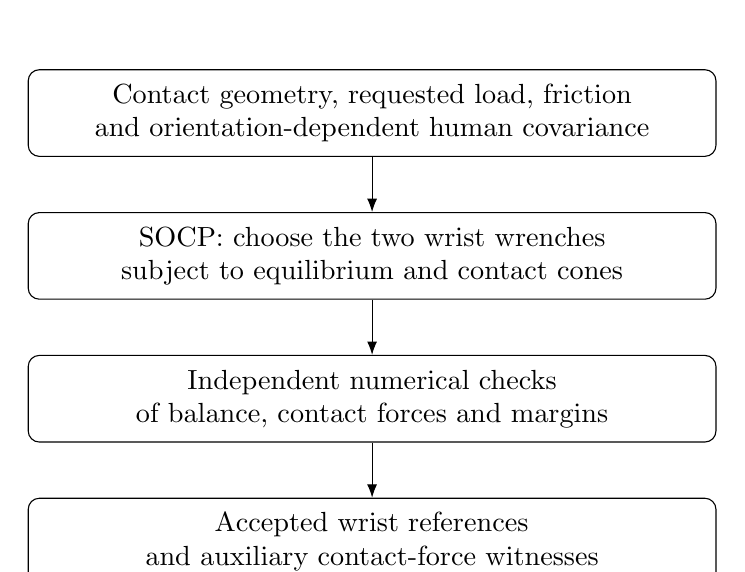
\begin{tikzpicture}[node distance=7mm,box/.style={draw,rounded corners,align=center,text width=85mm,minimum height=11mm},>=Latex]
\node[box] (inputs) {Contact geometry, requested load, friction\\and orientation-dependent human covariance};
\node[box,below=of inputs] (solve) {SOCP: choose the two wrist wrenches\\subject to equilibrium and contact cones};
\node[box,below=of solve] (check) {Independent numerical checks\\of balance, contact forces and margins};
\node[box,below=of check] (out) {Accepted wrist references\\and auxiliary contact-force witnesses};
\draw[->] (inputs)--(solve);\draw[->] (solve)--(check);\draw[->] (check)--(out);
\end{tikzpicture}
\caption{One local allocation. A failed solve or failed numerical check rejects the candidate. Acceptance establishes feasibility under the supplied model; the execution layer must still realize the accepted wrench through the arms and passive tools.}
\label{fig:socp-blocks}
\end{figure}

The twelve wrist components are the physical output of interest. The eighteen auxiliary pad-force components certify that the chosen wrench pair can be supported by the assumed point contacts. An implementation may eliminate $\vect w$ by substituting $\vect w=H\vect f$ and solve directly for those eighteen components; this is the same wrist objective expressed in different variables. It does not provide eighteen independently actuated commands. The human mean is not a reference force: only the covariance enters the active cost.

Evaluation has three separate levels. First, numerical acceptance checks equilibrium and each contact constraint in their stated units. Second, execution compares measured wrist wrenches with the accepted references, reporting tracking error, transients, force minima and command saturation. Third, the task is judged after release: whether the object remains supported and where it comes to rest. A low objective value, a feasible status and a small mean force bias are not substitutes for these physical measurements.

The SOCP receives the pad--object contacts, not a complete collision scene. It cannot infer which shelf edge a future motion will meet. For insertion, the scene and the route model predict an external load before allocation, as explained in Section~\ref{sec:insertion-load-source}. Unexpected contacts can therefore invalidate the supplied load without making the numerical solve incorrect. Chapter~\ref{ch:kinova} distinguishes online reallocation from an offline wrench plan followed with measured-force feedback.


\section{Decision variables: two wrist wrenches}

The robot does not command individual pads. Each hand is a passive tri-pad tool on a compliant wrist, and the controller tracks one wrench per wrist. The decision vector is therefore
\begin{equation}
\vect w=\begin{bmatrix}\vect F_L^\top&\vect\tau_L^\top&\vect F_R^\top&\vect\tau_R^\top\end{bmatrix}^\top\in\R^{12},
\end{equation}
where $\vect F_h$ is the world-frame force that hand $h$ applies to the object and $\vect\tau_h$ is the moment about its own measured wrist pole $\vect b_h$.

The three pads of each hand enter only as auxiliary variables. For $h\in\{L,R\}$ and $j\in\{1,2,3\}$, let $\vect f_{hj}\in\R^3$ be the force of pad $j$ on the object, and let
\begin{equation}
H_h\vect f_h=\begin{bmatrix}\sum_j\vect f_{hj}\\ \sum_j(\vect p_{hj}-\vect b_h)\times\vect f_{hj}\end{bmatrix}
\label{eq:hand-map}
\end{equation}
sum the three point forces and their moments about the wrist. The constraint $H_h\vect f_h=\vect w_h$ states that the wrist wrench must be producible by three Coulomb point contacts. The eighteen pad components are feasibility witnesses: they prove that such forces exist, but they are not commands and they are not penalized. Whether the passive tool distributes the load as the witness does is a separate question of realization, measured in Chapter~\ref{ch:evidence}.

There are no independent pad moments. Torsion about a hand axis arises only from the moments of the three point forces, as derived in Chapter~\ref{ch:contacts}. This keeps the coupling between vertical support and torsional capacity.

\section{Exact equilibrium about the estimated CoM}

Let $\hat{\vect p}_c$ be the estimated CoM and $\vect r_h=\vect b_h-\hat{\vect p}_c$. The two balance equations are
\begin{align}
\vect F_L+\vect F_R&=\vect b_F,\nonumber\\
\crossmat{\vect r_L}\vect F_L+\vect\tau_L+\crossmat{\vect r_R}\vect F_R+\vect\tau_R&=\vect b_\tau.
\label{eq:wrist-balance}
\end{align}
In the air the hands must supply the weight with no moment about the believed CoM: $\vect b_F=-\hat m\vect g$, $\vect b_\tau=\vect 0$. During placement, once support is detected, $\vect b$ becomes gravity minus a tared estimate of the support wrench obtained from the wrists. This changes the requested load, not the equations, the decision variables or the objective. It is a quasi-static estimate of the remaining load, not an independent support sensor.

The CoM is believed, not necessarily true. A zero moment target is correct about that point under the estimated gravity model. Writing the same target about the grasp centre when the CoM is offset would solve the wrong equilibrium.

Equation~\eqref{eq:wrist-balance} is a hard equality. Unlike the earlier formulation, there is no equilibrium slack. If the active contacts cannot balance the requested wrench inside the cones, the solver returns infeasible and the allocation is rejected. A mismatch is no longer hidden as a small residual inside an \sourcefile{optimal} status.

\section{The hand wrench cone}

For an active pad with unit outward normal $\vect n_{hj}$, compression and tangential force are
\begin{equation}
\lambda_{hj}=-\vect n_{hj}^\top\vect f_{hj},\qquad
\vect f_{t,hj}=\vect f_{hj}+\lambda_{hj}\vect n_{hj}.
\label{eq:normal-tangent}
\end{equation}
The normal points out of the object and the compressive force points into it, so $\lambda_{hj}\geq0$ forbids pulling through a nonadhesive contact. The admissible wrenches of hand $h$ are
\begin{equation}
\mathcal W_h=\Bigl\{H_h\vect f_h:\
\norm{\vect f_{t,hj}}_2\leq\mu\lambda_{hj}-\rho_{hj}\sqrt{1+\mu^2}\ \text{if }a_{hj}=1,\quad
\vect f_{hj}=\vect0\ \text{if }a_{hj}=0\Bigr\},
\label{eq:hand-cone}
\end{equation}
with active-contact flags $a_{hj}$ and margins $\rho_{hj}\geq0$ defined in the next section. With $\rho_{hj}>0$ the inequality already implies $\lambda_{hj}>0$. A detached pad keeps its slot in the model but carries no load. The solver rejects a configuration in which either hand has no active pad.

The friction inequality is applied to each of the six contacts separately. Aggregating a hand first and checking only its resultant would lose the individual normals and let one pad's excess tangential demand hide behind another.

The floating plate adds one constraint. Its mount transmits no bending at the contact centre, so for that tool the moment of the three pad forces about their centroid must have no component perpendicular to the mean normal. The rigid tool has no such condition.

\section{Signed friction margins: cones shifted inward}
\label{sec:signed-margin}

A contact force exactly on the boundary of its cone is about to slip. Any error in the normal estimate, the friction coefficient or the realized force can push it outside. The allocator therefore keeps a margin. The construction follows \citet{frictioncone2026}, with a three-dimensional adaptation described below.

\paragraph{Signed distance.}
For a force $\vect f$ at a contact with friction $\mu$, define
\begin{equation}
\psi_\mu(\vect f)=\frac{\mu\lambda-\norm{\vect f_t}}{\sqrt{1+\mu^2}}.
\label{eq:signed-distance}
\end{equation}
It is positive inside the cone, zero on its surface and negative outside. Its unit is newtons: away from the apex it is the Euclidean distance in force space from $\vect f$ to the cone surface. The gradient of $\psi_\mu$ has unit norm wherever $\vect f_t\neq\vect0$, so $\psi_\mu$ is $1$-Lipschitz. The constraint in Equation~\eqref{eq:hand-cone} is exactly $\psi_\mu(\vect f_{hj})\geq\rho_{hj}$.

\paragraph{What the shift guarantees.}
If $\psi_\mu(\vect f)\geq\rho$ and $\norm{\delta\vect f}\leq\rho$, then
\begin{equation}
\psi_\mu(\vect f+\delta\vect f)\geq\psi_\mu(\vect f)-\norm{\delta\vect f}\geq0.
\end{equation}
Every force deviation up to $\rho$ newtons in any direction keeps the contact inside the nominal cone. The guarantee holds for a fixed contact frame and a correct $\mu$. Changes of the normal, slip and the passive realization of the witness forces lie outside it.

\paragraph{Shifted, not narrowed.}
Figure~\ref{fig:friction-section} compares the two ways of reserving friction. The earlier formulation scaled the slope to $(1-r_s)\mu$. The apex stays at the origin, so a contact with small compression keeps almost no distance from slip, and the reserve grows only in proportion to the load. The signed margin keeps the opening angle $\arctan\mu$ and moves the apex inward along the normal, to
\begin{equation}
\lambda_{\min}=\frac{\rho\sqrt{1+\mu^2}}{\mu}.
\end{equation}
Every admissible force is then at least $\rho$ from the nominal boundary, including lightly loaded ones, and an active pad cannot be planned with zero load. With $\mu=1$ and $\rho=1$ N, $\lambda_{\min}\approx1.41$ N.

\begin{figure}[htbp]\centering
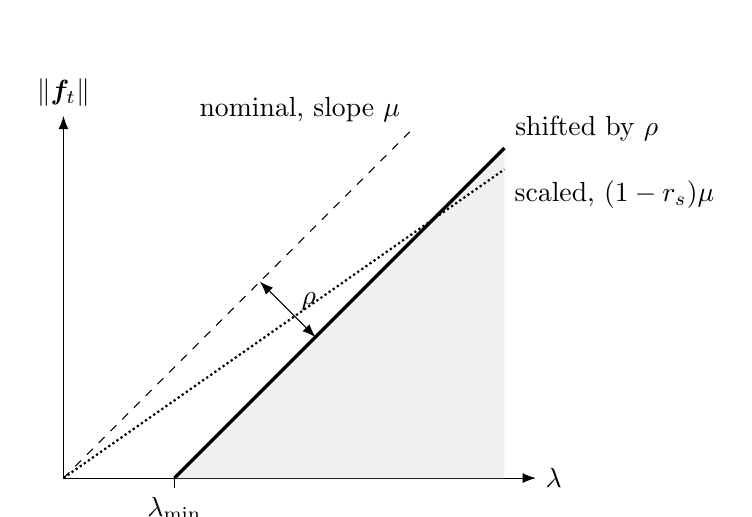
\begin{tikzpicture}[>=Latex,scale=1.0]
\draw[->] (0,0)--(6.0,0) node[right] {$\lambda$};
\draw[->] (0,0)--(0,4.6) node[above] {$\norm{\vect f_t}$};
\fill[gray!12] (1.41,0)--(5.6,4.19)--(5.6,0)--cycle;
\draw[dashed] (0,0)--(4.4,4.4) node[above left] {nominal, slope $\mu$};
\draw[thick,densely dotted] (0,0)--(5.6,3.92) node[right,yshift=-9pt] {scaled, $(1-r_s)\mu$};
\draw[very thick] (1.41,0)--(5.6,4.19) node[right,yshift=7pt] {shifted by $\rho$};
\draw[<->] (3.2,1.79)--(2.495,2.495);
\node[right] at (2.9,2.25) {$\rho$};
\draw (1.41,0)--(1.41,-0.12) node[below] {$\lambda_{\min}$};
\end{tikzpicture}
\caption{A section of friction admissibility at $\mu=1$. The dashed line is the nominal Coulomb boundary. The dotted line is the scaled cone of the earlier formulation, here $r_s=0.30$, whose apex stays at zero compression. The solid line is the signed-distance cone: same opening, apex moved inward so that every admissible force lies at least $\rho$ from the nominal boundary. The shaded region is the shifted admissible set. The two reserved cones cross: at high compression the scaled cone is the stricter one, at low compression it leaves almost no distance from slip.}
\label{fig:friction-section}
\end{figure}

\paragraph{Task-adaptive size.}
A single constant $\rho$ would be too small for a heavy object and too large for a light one. The paper scales the margin with the task. Our lift and wield are in the air and balance six axes at the estimated CoM, so we port the general-task adaptation of its appendix, as implemented for the Kinova experiments. Let $A$ be the force-only grasp map about $\hat{\vect p}_c$, restricted to the columns of active pads, and $A^+$ its pseudoinverse. Then
\begin{align}
\vect f_{\mathrm{task}}&=A^+\vect b, &
\rho_{\mathrm{task}}&=0.25\,\norm{\vect f_{\mathrm{task}}}+1\ \mathrm{N},\nonumber\\
P&=A^+A, &
\rho_{hj}&=\norm{P_{hj}}_2\,\rho_{\mathrm{task}},
\label{eq:task-margin}
\end{align}
where $P_{hj}$ is the block of three rows of $P$ that belongs to pad $hj$. The modeled deviation set is $\{A\vect u:\norm{\vect u}\leq\rho_{\mathrm{task}}\}$: wrench errors on the object of bounded size. The correction $-P\vect u$ that absorbs such an error changes pad $hj$ by at most $\rho_{hj}$, which is what the shifted cone tolerates. For a scalar task this reduces to $\norm{G_i}/\norm{G}\,\rho_{\mathrm{task}}$, the paper's own expression. For the plate, deviations must also preserve zero bending; the map is built on the kernel of the bending constraint, so corrections do not bend the mount.

The margins are computed before the solve, from measured geometry and the estimated load. They never depend on the squeeze chosen by the optimizer. A task that the active contacts cannot balance at all is rejected at this step, before optimization.

\paragraph{What the margin is not.}
The scale $0.25$ is the paper's value. The floor of $1$ N was a tuning choice of the Kinova implementation, not a value mandated by the paper. The deviation set is a design set, not a calibrated bound on sensor or geometry errors, and the margin is not a probability of safety. It is a declared reserve whose effect has to be measured, as done in Section~\ref{sec:margin-comparison}.

\section{The objective: human precision only}

The cost is a quadratic form in the twelve wrist components:
\begin{equation}
J(\vect w)=\vect w^\top W(R)\,\vect w,\qquad
W(R)=T_R^\top\,\Sigma_{\mathrm{TP\text{-}GMM}}(R)^{-1}\,T_R,
\label{eq:wrist-objective}
\end{equation}
where $\Sigma_{\mathrm{TP\text{-}GMM}}(R)$ is the session~C covariance of Chapter~\ref{ch:prior} queried at the current attitude $R$, and $T_R=\diag(R^\top,R^\top,R^\top,R^\top)$ expresses world-frame wrenches in the axes of the prior. The implementation normalizes forces and moments by the human scales before forming the matrix; that scaling cancels algebraically and does not add another metric. A matrix that is not positive definite in all twelve components is rejected.

The cost contains no human mean, no contact-effort term, no added identity and no slack penalty. Directions in which the demonstrations varied little are expensive; directions in which they varied much are cheap. Equilibrium and the cones decide what is admissible; the prior decides which admissible wrench pair is preferred.

\paragraph{Why no effort term is needed.}
The earlier formulation needed an effort term because its prior cost was blind to the pad forces that leave both wrist wrenches unchanged (Section~\ref{sec:socp-previous}). Here the cost acts only on what is commanded, the wrist wrenches, and the witness forces are not penalized at all. The squeeze that keeps the object held comes from the constraints: equilibrium requires the weight to be carried through friction, and the shifted cones require each active pad to stay a distance $\rho_{hj}$ inside its cone. Without a margin nothing in the program asks for grip beyond the minimum, and the nominal arm of Section~\ref{sec:margin-comparison} shows the consequence.

\paragraph{The complete program.}
\begin{equation}
\begin{aligned}
\underset{\vect w,\ \vect f}{\operatorname{minimize}}\quad&\vect w^\top W(R)\,\vect w\\
\text{subject to}\quad&\text{Equation~\eqref{eq:wrist-balance}},\qquad H_h\vect f_h=\vect w_h,\\
&\norm{\vect f_{t,hj}}\leq\mu\lambda_{hj}-\rho_{hj}\sqrt{1+\mu^2}\quad\text{if }a_{hj}=1,\\
&\vect f_{hj}=\vect0\quad\text{if }a_{hj}=0,\\
&\text{zero bending at the plate centre (plate only)}.
\end{aligned}
\label{eq:wrist-socp}
\end{equation}
The candidate pipeline uses $\mu=1$ between pad and object, the task-adaptive margin of Equation~\eqref{eq:task-margin}, and the solvers CLARABEL, ECOS and SCS in that order.

\section{Acceptance}

Solver status alone does not accept a solution. After every solve, the returned numbers are checked independently of the solver: equilibrium of the witness forces and of the wrist wrenches about the estimated CoM, the linkage $H_h\vect f_h=\vect w_h$, compression, the shifted cone on every active pad, zero force on inactive pads and, for the plate, zero bending. The tolerances are numerical, $10^{-4}$ N for forces and contact constraints and $10^{-5}$ Nm for moments; they absorb convergence error and are not sensor noise. An \sourcefile{optimal_inaccurate} result is accepted only if every check passes. A separate execution audit recomputes the margins from the inputs and does not trust the margin reported by the solver.

The source of the active allocator is \sourcefile{lorenzo_data_analysis/full_wrench_socp/lib/socp.py}, and the margin construction is in \sourcefile{lib/friction_margin.py} of the same package. The script \sourcefile{check_socp.py} verifies the precision-only objective on the actual session~C model at three attitudes.

\section{Shifted against scaled and nominal cones}
\label{sec:margin-comparison}

The margin was compared on a fixed regression panel before it became the default. Five objects were selected before any result was seen: the flat cube \#1 and \#5, the jittered cube \#0 with two displaced corners, the long box \#2 and polytope \#3 of the 20--50-face band. Each was run with the fixed tri-pad, the fixed tri-pad with remote impedance (RCC, Section~\ref{sec:remote-impedance}) and the floating plate, under three cone settings: 45 runs. The settings were
\begin{itemize}
\item \emph{nominal}: Coulomb cone, $r_s=0$, $\rho=0$;
\item \emph{scaled}: the previous narrowing, $r_s=0.30$, $\rho=0$, that is $70\%$ of the friction opening;
\item \emph{shifted}: the signed-distance margin of Section~\ref{sec:signed-margin}, $r_s=0$.
\end{itemize}
View noise, arrival, estimator, motion, release and scoring were identical; only the cone changed. A clean success requires the physical endpoint, meaning hands clear, a verified supported rest and actual CoM error at most $20$ mm, together with zero failed solves and zero audit rejections. A placement reached after a failed solve and fallback is counted as physical but not clean.

\begin{table}[htbp]\centering\small
\begin{tabular}{@{}lccc@{}}\toprule
& Nominal & Scaled ($r_s=0.30$) & Shifted ($\rho$)\\\midrule
Clean successes, fixed tri-pad & 0/5 & 0/5 & 2/5\\
Clean successes, RCC & 0/5 & 1/5 & 3/5\\
Clean successes, plate & 0/5 & 2/5 & 2/5\\
\textbf{Clean successes, total} & \textbf{0/15} & \textbf{3/15} & \textbf{7/15}\\
Physical endpoint, total & 0/15 & 5/15 & 8/15\\
Failed solves, summed over runs & 3 & 135 & 11\\
Object lost during wielding & 1 & 0 & 0\\
Contacts while wielding$^{a}$, fixed & --- & 4.89 & 6\\
\quad RCC & --- & 4.17 & 6\\
\quad plate & --- & 6 & 6\\
\bottomrule\end{tabular}
\caption{Paired regression panel of 20 October 2026: five selected objects, three tools, three cone settings. Simulation only; not a population success rate. $^{a}$Median over the five objects of each run's mean measured contact count. The wield supervisor of that date was active in every arm and stopped most nominal runs. The panel report does not give a contact count for the nominal arm. Source: \sourcefile{full_wrench_socp/reports/signed_margin_20261020_43/} and \sourcefile{FRICTION_MARGIN.md}.}
\label{tab:margin-comparison}
\end{table}

Table~\ref{tab:margin-comparison} supports three observations.

First, the nominal cone gives no clean success and no physical placement. With $\rho=0$ the program has no reason to squeeze beyond the minimum, and the allocated forces sit on the boundary of the cone. The supervisor active at the time stopped twelve of the fifteen nominal runs during wielding, and one plate run lost the object.

Second, narrowing the cone helps, but it fails often in the solver: 135 failed solves over the panel, concentrated in a few runs (74 in one RCC run). Narrowing removes admissible directions without adding compression, so the problem becomes infeasible more often when contacts are few or poorly oriented.

Third, the shifted cone gives the most clean outcomes and keeps all six contacts in the median while wielding. The jittered cube places cleanly with all three tools (3.4, 2.1 and 1.7 mm), whereas with the scaled cone the fixed tri-pad and RCC stop wielding on that same object. The eighth physical placement, fixed cube \#5 at $8.9$ mm, used eleven fallbacks and is excluded from the clean count. No accepted shifted-cone solution was rejected by the independent audit; the largest accepted cone violation was $4.1\times10^{-7}$ N.

The panel does not show that the margin solves placement. The long box failed support qualification with all three tools, the polytope was stopped during wielding with the fixed and RCC tools, and with the plate it reached placement but timed out while unloading. Plate cube \#5 was stopped during wielding. More preload also raises the measured wrench peaks; the margin buys reserve with force. On this evidence the task-adaptive margin became the default at every entry point, with the scaled cone kept only as an explicit baseline. A smoke test with the new default and no overrides then placed cube \#1 with all three tools at 0.8, 1.5 and 0.8 mm, with no failed solve.

Two limits must be stated. The panel is five selected objects, not a population; no broad sweep with a frozen controller has been run. And the wield supervisor of that date, which held, retraced or stopped the motion on low reserve, is no longer part of the controller: cone reserve is now logged as a diagnostic only. The numbers of Table~\ref{tab:margin-comparison} compare cones under that supervisor and are not results for the current policy.

\section{Realizing the allocation}

The optimizer supplies two wrist wrenches. The wrist controller tracks them through measured-wrench feedback on the compliant wrist, and the passive pads distribute the load by contact mechanics. The witness forces are not commanded, so the realized pad distribution can differ from the planned one. The shifted cone forbids a planned pad with zero load whenever its margin is positive, but it does not force the passive tool to load that pad. Contact counts, the error between planned and measured wrist wrench, and lost contacts must therefore be reported as measurements, not assumed from feasibility.

\section{The previous formulation: eighteen forces, slack and a scaled cone}
\label{sec:socp-previous}

The geometry campaign of Chapter~\ref{ch:geometry} and the Tetris insertion of Chapter~\ref{ch:tetris} used an earlier allocator. Its decision variables were the eighteen pad forces themselves, plus force and moment slack $\vect s_F,\vect s_T\in\R^3$. It differed from the active formulation in four ways.

\paragraph{Scaled cone, floor and cap.}
Each active pad obeyed
\begin{equation}
\norm{\vect f_{t,hi}}_2\leq(1-r_s)\mu\lambda_{hi},\qquad \lambda_{hi}\geq f_{\min},\qquad \norm{\vect f_{hi}}_2\leq f_{\max},
\label{eq:friction-cone}
\end{equation}
with $r_s=0.10$ in the passive-tool and Tetris allocators, a default floor of $1$ N and a per-pad cap
\begin{equation}
f_{\max}=35\ \mathrm{N}.
\label{eq:pad-cap}
\end{equation}
The floor was clipped to $0.9f_{\max}$ to avoid a contradiction with the cap. The cap bounded the total force norm, so the three compressions of one hand could not exceed $105$ N. With $\mu=0.49$, the slope used for allocation was $0.441$.

\paragraph{Soft equilibrium.}
Balance about the believed CoM was written with slack:
\begin{align}
\sum_{h,i}\vect f_{hi}&=\vect F_d+\vect s_F,\nonumber\\
\sum_{h,i}(\vect p_{hi}-\hat{\vect p}_c)\times\vect f_{hi}&=\vect T_d+\vect s_T.
\label{eq:slack-balance}
\end{align}
The program was therefore always solvable, and an allocation was accepted only if $\norm{\vect s_F}<0.5$ N and $\norm{\vect s_T}<0.05$ Nm.

\paragraph{Objective with effort.}
With $F_0=\hat m g_0$, $T_0=F_0r_0$, $r_0=0.05$ m and $\vect d_n$ the normalized deviation of the wrist wrenches from the human mean,
\begin{equation}
J=\frac{w_F}{F_0^2}\sum_{h,i}\norm{\vect f_{hi}}^2
+\frac{w_P}{2}\vect d_n^\top Q_n(R)\vect d_n
+w_S\left(\frac{\norm{\vect s_F}^2}{F_0^2}+\frac{\norm{\vect s_T}^2}{T_0^2}\right),
\label{eq:full-objective}
\end{equation}
with $w_F=w_P=1$ and $w_S=10^4$. The effort term was necessary there. The map from eighteen pad forces to twelve wrist coordinates has a kernel, and a prior-only cost would have been blind to the pad forces in it. In the active formulation the pad forces are not decision variables of the cost, so the term is no longer needed.

\paragraph{Its audit.}
The previous allocator was audited independently over the geometry campaign. Table~\ref{tab:socp-audit} is kept as the record of the non-shifted, scaled-cone allocator.

\begin{table}[htbp]\centering\small
\begin{tabular}{@{}lr@{}}\toprule
Allocations solved, all 1456 runs & 3\,432\,786\\
\quad CLARABEL \sourcefile{optimal} & 3\,430\,541\\
\quad CLARABEL \sourcefile{optimal_inaccurate}, residuals passing & 2\,221\\
\quad SCS \sourcefile{optimal} & 24\\
Accepted by the solver, rejected by the independent check & 0\\
Non-finite force values & 0\\
Largest force / moment residual of an accepted solution & 0.500 N / 0.050 Nm\\
Largest cone use $\norm{\vect f_t}/(\mu f_n)$ & 0.900\\
Largest deviation of a contact normal from unit length & $<10^{-6}$\\
\bottomrule\end{tabular}
\caption{Independent audit of the previous, scaled-cone allocator over the geometry campaign ($r_s=0.10$). Solvers are tried in the order CLARABEL, ECOS, SCS with library default tolerances (SCS: $\epsilon=10^{-5}$, 20\,000 iterations); ECOS was never needed.}
\label{tab:socp-audit}
\end{table}

The audit never overturned the solver. The largest cone use, 0.900, equals $1-r_s$: the optimum sat on the narrowed cone whenever friction was binding, which is precisely where a scaled cone leaves the least distance from slip at low compression. The fallback fraction, the share of control ticks with no applied allocation, was between 1 and 8\% on the polytopes and 23\% when the colliding plate added an unmodelled contact (Table~\ref{tab:plate-collision}). The largest accepted residuals, 0.5 N and 0.05 Nm, are the acceptance thresholds themselves: soft equilibrium let a small imbalance through by design. The active formulation removes both features, using exact equilibrium and a margin measured as a distance.

In that allocator the realization was a scalar squeeze loop on $F_{\mathrm{req}}=\max(\sum_i\lambda_{Li},\sum_i\lambda_{Ri})$, with a finite fallback squeeze ($21$ N in the blind script) when the allocation was rejected.

\section{Remote Cartesian impedance for the fixed tri-pad}
\label{sec:remote-impedance}

The compliant wrist is itself a feedback controller. Its original translational spring acts at the wrist, independently of the rotational spring. Active re-alignment changes a reference from contact normals; it does not relocate that compliance centre. An additional experimental arm instead shapes the compliance at the known centre of the three pad spheres, following the remote-compliance principle of \citet{whitney1982}. This arm uses the same allocator as the arm it is compared with.

Let $\vect r=(0.020,0,0)^\top$ m in the tool frame, and let $(\vect p,R)$ and $(\vect p_d,R_d)$ denote measured and commanded wrist poses. Define
\begin{align}
\vect c&=\vect p+R\vect r, & \vect c_d&=\vect p_d+R_d\vect r,\\
\vect e&=R_d^\top(\vect c-\vect c_d), & \vect\phi&=\operatorname{Log}(R_d^\top R)^\vee,\\
U&=\tfrac12 k_p\vect e^\top\vect e+
\tfrac12\vect\phi^\top K_r\vect\phi,
&K_r&=\diag(40,k_{\mathrm{tilt}},k_{\mathrm{tilt}}).
\end{align}
The remote point is apparatus geometry; actual sphere--surface contact points need not coincide with its plane. With $J_l$ the left Jacobian of $SO(3)$, the wrist wrench is
\begin{align}
\vect v_c&=\vect v+\vect\omega\times R\vect r,\\
\vect F&=-k_p(\vect c-\vect c_d)-k_d\vect v_c,\\
\vect T&=(R\vect r)\times\vect F
-R_dJ_l(\vect\phi)^{-\top}K_r\vect\phi-k_{dr}\vect\omega.
\label{eq:rcc-wrench}
\end{align}
Known tool gravity is compensated separately. No object vision, mesh, true mass or true CoM enters this law. The initial coarse-centre sensor remains part of the surrounding blind approach, and is a distinct declared input.

For fixed references and gains, away from the rotation-log cut at $\pi$, the elastic wrench is the negative gradient of $U$. Its power is $-\dot U$ and damping dissipates $k_d\norm{\vect v_c}^2+k_{dr}\norm{\vect\omega}^2$. Locally,
\begin{equation}
K_{\mathrm{wrist}}=\mathcal B^\top
\diag(k_pI,K_r)\mathcal B,\qquad
\mathcal B=\begin{bmatrix}I&-\crossmat{\vect r}\\0&I\end{bmatrix}.
\end{equation}
This positive-definite stiffness contains the translation--rotation coupling absent from a diagonal wrist spring. A pure tilt couple rotates about the remote point to first order. Torsional stiffness remains $40$ Nm/rad. The commanded-frame gains otherwise remain those of the reference rig.

The energy statement applies to the ideal continuous coupling with fixed references. The outer feedback loops, moving trajectories, gain transitions, sampled integration and contact changes are not covered by it. Retaining the torsional gain does not establish that the prior transfers without error to this altered apparent impedance. Both transmission and performance require measurement. The implementation is \sourcefile{lorenzo_data_analysis/10_tripad_passivo/lib/rcc.py}; finite-difference gradients, dissipation, frame covariance and free-tool linear sampled stability are checked independently.

\section{What is and is not constrained}

The active program constrains exact equilibrium about the estimated CoM, the producibility of each wrist wrench by three point contacts, compression, friction with a signed margin on every active pad, zero force on detached pads and, for the plate, zero bending. It has no force cap, no compression floor beyond the one implied by the margin, and no slack. It does not optimize spring travel, contact persistence, object deformation, damage, joint torque, arm collision, velocity or CoM uncertainty. Some are checked elsewhere; some remain unvalidated. A statement that the SOCP ``contains all physical limits'' would therefore be incorrect.

The useful guarantee is narrow and concrete: for fixed valid inputs, the witness forces lie at least $\rho_{hj}$ inside each nominal cone and balance the requested wrench exactly, to solver accuracy. A force deviation of that size at fixed geometry cannot by itself cause slip. Whether the realized forces stay within that deviation depends on estimation, measurement and transmission. This distinction is the basis of the experimental chapter.

\chapter{Experimental Evidence and Its Limits}
\label{ch:evidence}

The experiments are organized around the interfaces of the pipeline. The first asks whether the apparatus transmits the moment that learning uses. The second asks whether more squeeze improves a compliant grasp. The third asks whether the current optimization can represent finite contact forces without confusing a solved problem with an executable grasp. The final application asks whether a trajectory learned in one environment transfers to the actual insertion apparatus.

The evidence in this chapter comes from saved analyses and a dated source snapshot. The blind geometry campaign, completed on 5 October 2026, is reported in Chapter~\ref{ch:geometry} and referred to here where it supersedes a pilot; insertion campaigns still running during manuscript preparation are not incorporated. Haption demonstrations involve a physical operator and physical haptic devices coupled to a simulated object. Passive-tool and insertion measurements discussed here are simulation studies unless stated otherwise. They are not demonstrations on two industrial robot arms.

\section{Recording quality in session C}

The valid prior is trained from thirteen unperturbed runs, 024--036. The saved session-C report provides the data-quality measures in Table~\ref{tab:session-c}. These measurements characterize the retained recording apparatus before any claim is made about a controller using its prior.

\begin{table}[htbp]\centering\small
\begin{tabular}{@{}lr@{}}\toprule
Session-C measure & Recorded value \\\midrule
Unperturbed runs & 13\\
Rotational coupling & 40 Nm/rad\\
Mean active pads & 5.01 of 6\\
Samples with all six pads & 30.9\%\\
Usable samples under the stated drift filter & About 90\%\\
Display saturation & About 1.1\%\\
Samples beyond $60^\circ$ tilt & 2.7\%\\
95th percentile of gravity tilt & $55^\circ$\\
Reported inertial/applied moment ratio & 0.40\%\\
\bottomrule\end{tabular}
\caption{Session-C quality indicators transcribed from the saved analysis. The percentages have different definitions and should not be combined into one quality score.}
\label{tab:session-c}
\end{table}

The inertial-moment ratio supports the quasi-static interpretation of the recorded task. It does not validate every sample or every later trajectory. The all-six-pad percentage also shows why the prior should not be described as a six-contact distribution at every instant. The drift filter retains useful portions of runs that contain slip instead of silently discarding the entire difficult run.

The empirical gravity coverage is limited. The report describes useful coverage within the moderate-tilt region, with a $55^\circ$ 95th percentile and a small tail beyond $60^\circ$. The distinction between a percentile and an absolute bound matters. ``Supported up to approximately $55^\circ$'' is appropriate; ``trained uniformly over all orientations'' is not.

\section{The coupling wrench is the spring signal}

The saved comparison reports a ratio of logged moment magnitude to stiffness times angular deflection of approximately one in every recording group. This confirms the definition of the logged channel. Table~\ref{tab:coupling-groups} lists the apparatus indicators.

\begin{table}[htbp]\centering\small
\begin{tabular}{@{}lrrrr@{}}\toprule
Group & $K_{p,R}$ & Deflection & Median $|\tau|$ & Pads/6\\
& Nm/rad & degrees & Nm & \\\midrule
Earlier recording & 0.5 & 31.4 & 0.27 & 6.00\\
Session A & 60 & 1.10 & 1.15 & 4.64\\
Session B & 40 & 1.92 & 1.34 & 4.72\\
Session C & 40 & 1.74 & 1.22 & 5.01\\
\bottomrule\end{tabular}
\caption{Saved comparison of rotational coupling and recording transmission. These are apparatus-specific summaries. The median-moment statistic differs from other moment summaries in the session report.}
\label{tab:coupling-groups}
\end{table}

The compliant configuration has the best contact count and the lowest transmitted moment. Relative to the session-C median, $0.27/1.22\simeq22\%$. This ratio quantifies attenuation in this comparison; it is not a universal transfer function of a spring with stiffness $0.5$ Nm/rad.

Mechanically, the proxy can rotate toward the object and reduce the required spring deflection. That helps the pads remain seated. Statistically, it reduces the recorded torsional variation. The apparent improvement in grasp quality therefore changes what the learning algorithm can observe.

\section{Directional UCM-related coordination index}

The comparison evaluates residual hand moments in a grasp basis, following the task-equivalent-variation interpretation in Section~\ref{sec:ucm-prior}. The scalar below is the implemented difference-mode index, not the classical whole-space UCM variance ratio~\cite{scholz1999}. Residuals are formed within gravity-direction cells so that deterministic load changes with orientation do not dominate the covariance. The matched analysis restricts the comparison to common cells.

Let $C_{LL},C_{RR}$ be the residual covariance blocks and $C_{LR}$ their symmetrized cross-covariance. For direction $\vect n$, the implemented index is
\begin{equation}
r(\vect n)=1-
\frac{2\vect n^\top C_{LR}\vect n}
{\vect n^\top C_{LL}\vect n+\vect n^\top C_{RR}\vect n}.
\label{eq:directional-r}
\end{equation}
Equivalently, it is the variance of the projected difference between the hands divided by the sum of their projected variances. Independent residuals give $r=1$. Positive covariance reduces $r$, indicating suppression of the difference mode. Negative covariance raises it, indicating more variation in that mode. The names ``retained'' and ``free'' describe this relative variance, not an absence or presence of a physical constraint.

\begin{table}[htbp]\centering\small
\begin{tabular}{@{}lcc@{}}\toprule
Residual direction & $K_{p,R}=0.5$ & $K_{p,R}=40$\\
\midrule
Torsion along grasp axis & 0.61 [0.34, 0.94] & 1.42 [1.29, 1.54]\\
Moment along $v$ & 0.15 [0.10, 0.23] & 0.99 [0.68, 1.26]\\
Moment along $w$ & 0.72 [0.60, 0.87] & 0.84 [0.63, 1.08]\\
\bottomrule\end{tabular}
\caption{Directional indices and reported confidence intervals from the matched saved analysis. The high-stiffness comparison combines the documented qualifying runs of sessions B and C; it is not the thirteen-run training set alone.}
\label{tab:ucm-comparison}
\end{table}

\thesisfigure[0.80]{ch08_evidence/torsional_index.pdf}{Torsional difference-mode indices reconstructed from Table~\ref{tab:ucm-comparison}. Error bars reproduce the reported confidence intervals. The unit reference marks independent residuals. No new statistical fit is represented.}{fig:torsional-index}

The torsional index changes from below to above one, with disjoint reported intervals. The saved run-level Mann--Whitney comparison gives $p=4.4\times10^{-4}$ for seventeen earlier runs and nineteen qualifying high-stiffness runs. Run-level distributions overlap; the result is not that every individual run changes class.

The force-direction indices remain high in both groups. In a settled lift, the net force is constrained by weight, so opposing hand fluctuations are expected. That agreement is a useful consistency check on frames and signs. It does not independently establish a sophisticated human synergy, because the force balance itself constrains the resultant.

\section{Effect on the learned cost}

The older model's moment scale is reported as $0.158$ Nm, compared with $0.716$ Nm for the valid session-C model. Their squared inverse-scale ratio is
\begin{equation}
\left(\frac{0.716}{0.158}\right)^2\simeq20.5.
\end{equation}
This explains the approximately twenty-one-fold scalar precision difference noted in the project. It is a scale-level comparison, not a claim that every eigenvalue of the full twelve-dimensional precision changes by the same factor.

A controller using the earlier precision would penalize torsional deviations as if they were much more repeatable. The issue is not solved by loading a model with the right matrix dimensions. The dataset, apparatus settings and output conventions must match the intended controller.

\section{A force ladder on one compliant grasp}

The documented comparison applies different per-hand squeeze levels to the same object and compliant-wrist setup.

\begin{table}[htbp]\centering
\begin{tabular}{@{}rl@{}}\toprule
Squeeze per hand & Documented terminal outcome\\
\midrule
105 N & Object expelled during lift\\
30 N & Transport reached\\
21 N & Complete pipeline reached\\
\bottomrule\end{tabular}
\caption{Force ladder on the same documented case. It establishes non-monotonic behaviour in that setup; it is not a population success-rate experiment.}
\label{tab:force-ladder}
\end{table}

The mechanism is consistent with Equation~\eqref{eq:force-tilt}. Squeeze can deflect the wrist, move the pads and worsen opposition. If rejection invokes a stronger fallback, the resulting loop reinforces the geometric defect. The highest force can therefore fail before the lower-force run.

The experiment supports the statement that force is not a free safety parameter. It does not determine a unique optimal squeeze for every object, nor does it show that $21$ N is generally sufficient. A replicated paired campaign would be needed to map the stable force range against wrist stiffness, contact geometry and load.

\section{Checks on the mathematical implementation}

The source audit verifies that the current optimizer includes per-pad cones, per-pad force caps, zero forces for inactive pads, positive effort on all eighteen contact variables and measured equilibrium slack. The prior query includes the between-component covariance term, physical rescaling and right-hand unmirroring. The estimator preserves prior uncertainty in unobserved directions.

Appendix~\ref{app:math} supplies numerical checks of the corresponding identities. These checks establish algebraic consistency, not physical validation. In particular, they do not establish that a scalar squeeze loop realizes the force vectors selected by the optimizer.

The weakest execution interface is therefore the difference between allocated and realized wrench. An accepted allocation should be accompanied by measured force error, moment error, contact utilization and the fraction of ticks using fallback. An \sourcefile{optimal} solver status alone is not a sufficient experimental outcome. The geometry campaign records all four on every control tick: on the floating plate the realized force error has a median of 3.6 N and the moment error 0.065 Nm (Table~\ref{tab:prior-ablation}), and the independent constraint audit of Table~\ref{tab:socp-audit} never rejected a solution the solver had accepted.

\section{Preliminary passive-plate campaign}

Two saved summary files contain eighteen jittered objects each, six per family. The comparison changes whether the triangular plate carries a collision shape. The values in Table~\ref{tab:plate-pilot} are direct counts from copied CSV files in the manuscript evidence folder.

\begin{table}[htbp]\centering\small
\begin{tabular}{@{}lrrr@{}}\toprule
Plate configuration & Recorded objects & Held & Estimator abstentions\\
\midrule
Visual plate, sphere contacts & 18 & 18 & 0\\
Colliding plate & 18 & 18 & 1\\
\bottomrule\end{tabular}
\caption{Counts in the saved pilot summaries. ``Held'' is the recorded pipeline flag, not a verified final placement outcome. The colliding-plate arm includes a possible extra load path and is not validation of a six-point contact model.}
\label{tab:plate-pilot}
\end{table}

These counts are not the final geometry campaign. They do not establish unseen-shape generalization, nor do they compare rigid and passive tools. Their immediate use is to expose a model violation: a plate can help hold an object while invalidating the force set supplied to the estimator. A good visible outcome can therefore coexist with an invalid measurement model.

The pilot is superseded by the geometry campaign of Chapter~\ref{ch:geometry}: frozen populations with a manifest of every generator draw, the contact audit of Table~\ref{tab:plate-collision}, the constraint audit of Table~\ref{tab:socp-audit}, and a paired three-tool comparison on 182 bodies (Tables~\ref{tab:geo-mortality} and~\ref{tab:geo-paired}). Every planned run is in the ledger: 1456 runs, including two declared sensor-noise arms, none crashed and none missing. The generator rejected 21 polytope draws for size, a precondition of the arm opening and workspace; 2 more fell outside the declared face range, and nothing else was excluded. Three runs killed by an operating-system restart were rerun from scratch, and an earlier full launch, archived whole, reproduced every pre-release quantity of the 852 runs it shares with the final one exactly. The pilot's central observation survives on the population: the colliding plate places nearly as many bodies as the clean one while breaking the estimate on most polytopes.

\section{How failures will be reported}

Every object enters the ledger before approach. The report records first failure at approach, seating, lift, estimation, reorientation, transport or release. Estimator abstention is recorded separately from physical loss of the object. An abstention is an honest lack of information, but it still prevents completion when the next stage requires a three-dimensional estimate.

\begin{table}[htbp]\centering\small
\begin{tabular}{@{}lp{0.57\textwidth}@{}}\toprule
Stage & Quantity to record before final aggregation\\
\midrule
Population construction & Generated bodies, numerical rejections and apparatus exclusions.\\
Approach and seating & Bodies attempted, contact masks and non-pad contacts.\\
Lift & Drops, expulsions, accepted SOCP ticks and fallback use.\\
Estimation & Accepted samples, observed directions, clipping and abstentions.\\
Reorientation and transport & Contact losses, wrench errors and force peaks.\\
Release & Final pose error after hands are clear and the object has settled.\\
\bottomrule\end{tabular}
\caption{Reporting ledger. The geometry campaign reports every row (Chapter~\ref{ch:geometry}); no unmeasured stage count is filled in.}
\label{tab:mortality-protocol}
\end{table}

The scientific value of this reporting is causal. A population that never seats the tool is different from a population that seats it and later loses the object through wrist deflection. Conditioning on survivors would combine those mechanisms and inflate the apparent performance of later stages.

\section{Interpretation}

The strongest established findings concern apparatus dependence. Rotational compliance changes the recorded signal; squeeze changes the realized geometry; and additional unmodelled contact can improve holding while breaking estimation. These findings motivate the architecture. Claims about the net benefit of the human prior, arbitrary-shape handling and held-out insertion performance remain tied to their own controlled comparisons.


\chapter{From Boxes to Irregular Geometries}
\label{ch:geometry}

Geometry is introduced progressively so that a failure can be attributed to a change in the object rather than to several simultaneous changes in the apparatus. A perfect cube tests the pipeline without surface irregularity. A cube with one displaced corner tests a controlled local defect. Jittered corners remove the deliberately chosen defect direction. Random-plane polytopes then remove the assumption that the body is essentially box-like.

This chapter specifies each construction and reports a blind simulation campaign over all of them: 182 bodies, three end-effector configurations, three prior modes and two levels of sensor noise, 1456 runs in total. Every planned run is in the ledger, and every number below is regenerated from the per-run records by the campaign's report scripts. The campaign is a simulation in PyBullet; its limits are stated in Section~\ref{sec:geo-limits}.

\section{What the geometry progression tests}

The progression tests whether the allocator and passive tool tolerate a changing local contact set without assuming parallel faces. The cube provides a reference. One displaced corner isolates a seating defect. Jitter distributes variation across the body. Random-plane convex polytopes remove the box-like arrangement of opposing surfaces.

These are synthetic populations, not a documented manufacturing-tolerance distribution. A 21.6 mm corner displacement on a 120 mm body is a stress condition, not an ordinary precision-machining tolerance. Potential applications include rigid packages with damaged outer geometry and rigid irregular parts admitted by the tool's opening. Deformable cardboard, sharp concavities and shifting contents require additional models.

The outcome is whether conformity preserves a usable three-point load path, whether measured normals remain allocatable under finite force, and whether estimation survives without extra support. Paired comparisons and failures by stage attribute differences to the design rather than to the population.

\section{The information available to the planner}
\label{sec:geo-information}

A geometry experiment must state what the planner can access. A known-mesh arm can choose opposing faces using the mesh. A rough-size arm must use an explicitly perturbed size. A blind-search arm can approach from a coarse object location and discover contact through force feedback. These arms answer different questions and must retain separate results. Only the blind-search arm exists in this implementation, so only it was run; nothing below mixes information regimes.

The true simulated mass, CoM, facet set and body base position are prohibited inputs to a blind decision. In Bullet, the reported base position can be the inertial-frame CoM rather than the nominal geometric origin. Treating it as an ordinary object position can therefore leak the unknown quantity into control. An accessor audit must examine every use, including stage gates and population selection.

That audit was carried out on the entry point, the search, the allocator call, the estimator, the prior-frame construction and the stage gates. The planner, the estimator, the allocation and the prior query read only the coarse sensor of the geometric centre (with its declared 10 mm error), the contacts, the measured force and the solver status. One gate did read the truth: the checks that the object was still held after the lift and after the wielding compared the \emph{true} body height, and the wielding was entered only if the first check passed. It produced no visible defect, because the check was correct, which is precisely how such a leak hides. Both checks now use the same declared coarse sensor as the search, averaged over ten readings on its own random stream, and fall back to contact counts alone when no sensor is given; the true height is still written to the record, for reporting only. Over the campaign the new gate disagreed with the truth once in 30 wielding losses, on the safe side (20.0 mm seen against 5.3 mm true).

\section{Perfect cube: establishing the contact loop}

The perfect cube is a control experiment rather than a proof of generality. Its flat faces allow three parallel normals per hand when the triangle lies inside the face. That separates failures due to scalar-force realization, wrist deformation or estimation from failures due to changing facet normals.

Even a cube does not guarantee seating. A tool footprint near an edge can place one sphere outside the face. The search must account for the measured contact mask and should not assume that a visual cube supplies six contacts automatically.

The basic sequence is approach, seat, allocate squeeze, lift, estimate, wield, reorient, transport and release. Load identification and wielding remain free-space stages. Touchdown uses contact feedback only after the estimation interval has ended. Samples influenced by support are not allowed to enter the airborne regression. In the campaign every run performs this whole sequence: blind search, squeeze, a 150 mm lift, a $\pm35^\circ$ wielding cycle, a $90^\circ$ yaw, placement at a fixed target by force-guided lowering, release, and the pose measured once the hands are clear.

\section{The end-effector configurations}
\label{sec:geo-arms}

Three configurations are compared on every body. The \emph{fixed tri-pad} is the rigid three-sphere tool on the compliant wrist. It is run twice: without and with the wrist re-alignment controller, which during the approach re-commands the wrist orientation from the measured contact normals up to three times. The \emph{floating-plate tri-pad} carries the three spheres on a plate suspended by zero-rest-length springs and is never run with the re-alignment controller: the plate is designed to conform mechanically precisely so that this control layer is not needed, and running it with the controller would measure a controller and a mechanism together. The axial-travel tool of Chapter~\ref{ch:contacts} was excluded from the comparison by design decision. Every arm still uses wrist impedance and squeeze feedback; ``without controller'' here refers only to active wrist re-alignment. All arms share the friction coefficient, trajectories, estimator gates, mass band, target and sensor error, and the plate carries no collision shape unless declared otherwise (Table~\ref{tab:plate-collision}).

\section{The step before jittered boxes: one displaced corner}

A deterministic deformation moves one cube vertex by a known geometric construction while the other seven remain fixed. The displacement is an independent variable of the population generator; it is not information given to the blind controller. Reusing the same configuration at several displacement magnitudes produces a paired geometry comparison.

The saved geometric analysis shows why this step cannot be summarized by mean irregularity alone. Most axes still intersect a largely intact face, so median local unevenness can remain close to zero. The upper tail grows where the tool spans the deformed region or an edge. A localized defect tests rare poor seating rather than uniformly difficult seating.

Local unevenness can be defined by placing the nominal three-pad footprint against the body along a candidate direction and measuring the spread of contact depths. A pad directed into empty space is a separate category; it should not be assigned an arbitrary finite unevenness and merged into the same distribution.

In the campaign the corner direction (corner 7, along its own diagonal), the magnitudes, the arrivals and the tool settings are frozen. The 120 mm cube of 2 kg has its CoM 20 mm along the push direction, and the search seeds are the same for every magnitude, so between two bodies only the corner moves. Table~\ref{tab:one-corner} lists every run; none is selected.

\begin{table}[htbp]\centering\small
\begin{tabular}{@{}rrrlll@{}}\toprule
Push & Faces & p90 unevenness & Fixed, no align. & Fixed, align. & Floating plate\\
\midrule
0 mm & 6 & 0.0 mm & placed & lost in wielding & placed\\
+6 mm & 9 & 0.9 mm & placed & lost in wielding & placed\\
+12 mm & 9 & 4.8 mm & placed & placed & placed\\
+24 mm & 9 & 30.8 mm & placed & placed & placed\\
+48 mm & 9 & 54.5 mm & placed & placed & placed\\
$-36$ mm & 9 & 26.7 mm & placed & placed, $163^\circ$ off & placed\\
\bottomrule\end{tabular}
\caption{One displaced corner, deterministic. Every run seated 6/6 pads at the first attempt and no plate or flange contact occurred. The fixed tool with the controller loses the two \emph{least} deformed bodies in the wielding (true slip 54 and 65 mm); without the controller it places them. Bodies placed by the plate end within 11.5 mm and $1.1^\circ$ of the request.}
\label{tab:one-corner}
\end{table}

The controlled defect separates nothing on the floating plate: it places all six bodies within tolerance. The informative line is the fixed tool's: the re-alignment controller costs it the two easiest bodies, the perfect cube and the 6 mm push, which the same tool without the controller places. Re-commanding the wrist on contact moves the pads, and on a near-perfect face it is the only thing that moves them.

\section{Jittered corners: a bounded isotropic construction}

For each of the eight cube vertices, draw $\vect z_i\sim\mathcal N(\vect0,I_3)$ and $u_i\sim\mathrm{Uniform}(0,1)$. With edge length $L$ and jitter fraction $\delta$,
\begin{equation}
\vect v_i'=\vect v_i+\delta L\,u_i^{1/3}\frac{\vect z_i}{\norm{\vect z_i}}.
\label{eq:jitter-generator}
\end{equation}
The normalized Gaussian gives an isotropic direction. The cube root gives uniform volume density inside the displacement ball. The whole displacement is bounded by $\delta L$; it is not an independent bound of that size on each coordinate.

These choices matter. Normalizing a vector sampled uniformly inside a cube biases the directions toward its diagonals. Sampling radius uniformly concentrates more points near the centre than a uniform-volume distribution. An unbounded Gaussian displacement would also contradict the stated maximum jitter.

With the same seed, changing $\delta$ scales the same displacement directions and relative radii. This gives a paired comparison across jitter levels. With different seeds, the comparison is between populations as well as between amplitudes. The earlier three-family pilot used different seeds, so it was not a paired ladder; the campaign ladder is.

The campaign crosses two variables. The number of displaced corners is $k\in\{1,2,4,8\}$, where the corners are taken in a fixed per-pair order such that the first two share an edge and the first four form a whole face, so the sets are nested. The amplitude is $\delta\in\{0.05,0.10,0.18\}$, a bound of 6.0, 12.0 and 21.6 mm on $L=120$ mm. Each of eight pairs draws its directions, radii, corner order, mass (1--4 kg) and CoM direction (20 mm from the centre) once, and every $(k,\delta)$ cell reuses them; the pair index also fixes the search seeds. Between two cells of one pair, only the shape changes.

The convex hull of the displaced vertices remains the simulated body. A formerly square face can split into triangles when its vertices are no longer coplanar. Face counts depend on the coplanarity tolerance used to group hull triangles. Here hull triangles are one face when their normals agree within $0.5^\circ$ and their offsets within 0.2 mm, a tolerance checked against Euler's relation on generic polytopes. With it the jittered cubes have 8--9 faces at $k=1$, 9--10 at $k=2$, 9--11 at $k=4$ and 10--12 at $k=8$.

\thesisfigure{ch09_geometry/geometry_ladder.pdf}{Illustrative convex hulls for the geometry progression: a cube, one displaced corner, bounded jitter and a random-plane body. They are generated for explanation, not selected as successful campaign objects.}{fig:geometry-ladder}

\section{Random-plane convex polytopes}

The generator samples outward normals isotropically and intersects half-spaces,
\begin{equation}
\mathcal P=\left\{\vect x\in\R^3:
\vect n_j^\top\vect x\leq d_j,\ j=1,\ldots,N_p\right\},
\quad
\vect n_j=\frac{\vect z_j}{\norm{\vect z_j}}.
\label{eq:random-halfspaces}
\end{equation}
Plane offsets vary around a nominal radius. The implementation obtains the intersection, removes repeated vertices, constructs its convex hull and can apply anisotropic scaling. Some sampled planes can be redundant. The number of sampled planes is therefore not the number of final facets.

Adding three axis-aligned plane pairs would insert an artificial box structure and make parallel-face grasps unusually common. The current generator avoids that construction. Apparatus-size checks and numerical-degeneracy checks still constrain the generated population. They must be reported as part of the sampling process.

Because planes are not faces, the campaign bins polytopes by the number of faces \emph{measured} on the hull, with the coplanarity tolerance above: 10--20, 20--50, 50--100 and 100--200 faces, twenty bodies per band. The number of planes is drawn log-uniformly between 10 and 800, and each draw is assigned to the band of its measured face count. The band of 10--20 faces lies below the 20 faces suggested as a starting point in supervision and is kept as the lowest rung. All 146 draws are recorded with their outcome: 80 kept, 64 not used because their band was already full, 2 outside the declared range of 10--200 faces; the generator's own size check rejected 21 further draws. The campaign first ran ten bodies per band and then twenty; the sampling is sequential, so the first ten of each band are identical in both, and the earlier runs were kept. Masses are drawn in 1--4 kg and the CoM lies inside the body.

The generator supports irregular convex bodies, not arbitrary nonconvex geometry. Tetrominoes in the final application use a separate cell-based construction. A successful convex-polytope campaign would not by itself establish grasping of cavities, articulated parts, deformable packages or nonconvex unknown objects.

\section{Facet-specific contacts}

On a polytope, the three pads of one hand can touch different facets. Their normals can diverge even when their support positions form a triangle. The friction cone for each pad must use its own measured outward normal. Replacing all three by a single average normal can hide the very geometry that makes the allocation difficult.

The allocator receives one measured normal per pad, and the campaign records the widest angle between two pad normals of the same hand. On the jittered cubes its median is $6.5^\circ$ on the plate and $25.7^\circ$ on the fixed tool with the controller; on polytopes it is $55$--$66^\circ$ for every tool. On polytopes the three pads of a hand sit on different facets as a rule, not as an exception, and the allocation is solved on those distinct cones throughout.

The contact model and cap remain unchanged. Only the contact parameters change. The estimated CoM enters the moment balance, while the anchored grasp frame supplies the prior query. This separation allows the same local allocator to be used without assuming that a polytope has the same body frame or surface geometry as the training box.

The prior transfer was tested rather than assumed. Removing the prior term loses 51 bodies in the wielding against 15 (Table~\ref{tab:prior-ablation}). An equal-trace identity precision reproduces the learnt one on every cube-family body, and falls slightly behind it on polytopes. The box-trained precision does not hurt on irregular contacts, and on the most irregular ones it helps a little.

\section{Population selection and stage gates}

A population filter is an experimental decision. It can exclude objects that exceed the apparatus opening or the declared workspace. It must not exclude objects because their true CoM predicts failure or because a trial grasp was unsuccessful. Selecting only successful grasps would transform a population test into a survivor test.

\thesisfigure{ch09_geometry/polytope_zoo.pdf}{Bodies of the campaign population, drawn at a common scale. Top: the cube family, with the perfect $120$ mm cube dashed and moved corners in red. Bottom: the first body of each polytope face band. The bodies are taken in file order, not chosen by outcome.}{fig:polytope-zoo}

The generator also rejects degenerate or very small numerical hulls. Those counts should be recorded separately from apparatus exclusions. A facet-size filter, if used in an earlier arm, must be stated as that arm's precondition. It should not silently reappear in the passive-tool population, whose purpose is to tolerate nonplanar local seating. In the campaign the only filter is size, it rejected 21 polytope draws, and no facet-size or unevenness criterion selects any body; unevenness is recorded as a covariate. The face band is a declared stratification, not a filter on success; 2 draws fell outside it.

Per-run gates follow the same principle. Observability and contact measurements may cause abstention. True estimation error may only be computed after the gate. A threshold on true error would remove precisely the runs that the estimator needs to expose and would invalidate the downstream success rate.

\section{Results: where each configuration fails}
\label{sec:geo-results}

Table~\ref{tab:geo-mortality} counts, over every planned body, how many were placed and at which stage the others stopped. No run crashed and none is missing.

\begin{table}[htbp]\centering\small
\begin{tabular}{@{}llll@{}}\toprule
Family & Fixed, no align. & Fixed, align. & Floating plate\\
\midrule
One corner & 6/6 & 4/6 (2W) & 6/6 \\
Jitter, $k=1$ & 18/24 (6S) & 23/24 (1W) & 24/24 \\
Jitter, $k=2$ & 17/24 (7S) & 23/24 (1S) & 24/24 \\
Jitter, $k=4$ & 16/24 (7S, 1W) & 24/24 & 24/24 \\
Jitter, $k=8$ & 20/24 (4S) & 22/24 (2R) & 24/24 \\
Jitter, all & 71/96 (24S, 1W) & 92/96 (1S, 1W, 2R) & 96/96 \\
Polytopes, 10--20 faces & 8/20 (6S, 4L, 2W) & 15/20 (2S, 1L, 1W, 1P) & 14/20 (6W) \\
Polytopes, 20--50 faces & 17/20 (3S) & 14/20 (2L, 2W, 2R) & 17/20 (1L, 2W) \\
Polytopes, 50--100 faces & 19/20 (1W) & 16/20 (4W) & 17/20 (3W) \\
Polytopes, 100--200 faces & 18/20 (1S, 1W) & 19/20 (1L) & 15/20 (1L, 4W) \\
Polytopes, all & 62/80 (10S, 4L, 4W) & 64/80 (2S, 4L, 7W, 2R, 1P) & 63/80 (2L, 15W) \\
\bottomrule\end{tabular}
\caption{Placed bodies over every planned body, TP-GMM prior in all three arms. In parentheses, where the others stopped: S approach and seating, L lift, W wielding (estimation), R reorientation, P placement. Placed includes bodies placed on an edge.}
\label{tab:geo-mortality}
\end{table}

\begin{table}[htbp]\centering\small
\begin{tabular}{@{}lrrrr@{}}\toprule
Same body, arm A against arm B & A further & Same & B further & Sign test $p$\\
\midrule
Plate against fixed without controller & 46 & 122 & 14 & $<0.001$\\
Plate against fixed with controller & 29 & 138 & 15 & 0.049\\
Fixed with against without controller & 41 & 116 & 25 & 0.064\\
\bottomrule\end{tabular}
\caption{Paired comparison over the 182 bodies: on how many bodies one arm got to a later stage than the other. Two-sided exact sign test on the bodies where they differ.}
\label{tab:geo-paired}
\end{table}

\textbf{On the cube family the floating plate dominates, without active wrist re-alignment.} It places all 96 jittered cubes and all six one-corner bodies, at the first attempt with six seated pads. The fixed tool without the controller cannot seat on a jittered cube: 24 of its 25 failures are at the approach, after five attempts with only two or three pads seated. With the controller it seats, but it loses the easy bodies in the wielding and places only half of the jittered cubes within tolerance (below). The mechanism does what the controller does for the fixed tool, without moving the pads while doing it. The failures of the fixed tool are spread over every $k$ and every $\delta$, mild included; they do not grow with the amplitude, so the difficulty is that the faces are no longer flat, not how far the corners moved.

\textbf{On polytopes the three configurations are level.} They place 62, 64 and 63 of 80. One band separates two of them: on the 10--20-face bodies, few large and often elongated facets, the fixed tool without the controller fails to seat six times and the plate goes further on 13 bodies against 2 ($p=0.007$). Above 20 faces no band separates any pair. The plate's fifteen losses are all in the wielding: fourteen are drops of 126--171 mm and one is the sensor gate's false alarm. On many small facets the plate's conformity no longer buys an advantage. This is a negative result and is reported as one. With twenty bodies per band it is a statement that no difference was detected, not that the configurations are equivalent.

\textbf{Estimation follows the seating.} Over runs that finished the wielding the median CoM error is 0.05 mm on the jittered cubes and 0.21 mm on polytopes for the plate, against 1.2 and 1.5 mm (without controller) and 1.8 and 1.7 mm (with controller) for the fixed tool. The estimator abstained 0 and 5 times on the plate, 10 and 19 on the fixed tool with the controller, 4 and 22 without it. All accepted estimates observe three directions. The mass error is at most 0.2\%, which reflects a simulated wrench without sensor noise rather than the estimator.

\textbf{Sensor noise on the wrench does not change the outcome.} Two declared arms repeat the floating-plate runs on all 182 bodies with Gaussian noise added, per axis and per sample, to the wrench the estimator reads: 0.1 N and 0.005 Nm, about a good six-axis wrist sensor after filtering, and five times that. The contacts the allocator reads are left exact, so the arms isolate identification. Paired with the noise-free arm, the same stage is reached on 181 and 178 of 182 bodies ($p=0.62$ for the higher level), and 166 bodies are placed in both. The median mass error rises from below 0.01\% to 0.1\% and 0.4\% (worst 2.5\%), the median CoM error from 0.07 to 0.09 and 0.21 mm. Each estimate averages about a thousand quasi-static samples, so white noise of this size is averaged out; what this does \emph{not} test is a systematic error, bias or drift of a real sensor, which no amount of averaging removes.

\section{Placement after identification}

Once the object is reoriented, lowering should continue slowly until a measured support transition indicates that the environment is taking the load. The estimator is no longer updated as if all forces came from the hands. Release then reduces squeeze while observing whether the body remains supported.

For a known support polygon, static stability requires the gravity line through the CoM to lie inside that polygon. On a general blind polytope, the polygon may not be known. A support event and a settled pose are observations; they do not establish the same geometric criterion as a mesh-based stability calculation.

The final pose must be measured after the hands are clear. Measuring while the hands still constrain the body can report a commanded orientation that the object does not retain after release. Both requested and settled poses belong in the record. The campaign enforces this: the hands open, retreat 40 mm along their push axes and are held there while the body settles, and the record states whether any tool still touches the body when the pose is read. A body that remains leaning on a pad is its own outcome and is excluded from the pose errors. An earlier launch stepped the simulation without commanding the wrists during the settle, the uncommanded virtual couplings fell under gravity and a pad could land back on the body; that launch is archived and its pose columns are not used.

\begin{table}[htbp]\centering\small
\begin{tabular}{@{}lrrr@{}}\toprule
 & Fixed, no align. & Fixed, align. & Floating plate\\
\midrule
Jitter: placed / hands clear / within tolerance & 71 / 69 / 51 & 92 / 92 / 46 & 96 / 96 / 96\\
Jitter: position / attitude error, median & 11.2 mm / $3.6^\circ$ & 14.8 mm / $8.5^\circ$ & 6.2 mm / $3.5^\circ$\\
Polytopes: placed / hands clear / within tolerance & 62 / 60 / 22 & 64 / 62 / 26 & 63 / 56 / 30\\
Polytopes: position / attitude error, median & 11.3 mm / $11.8^\circ$ & 11.1 mm / $7.6^\circ$ & 10.1 mm / $7.6^\circ$\\
\bottomrule\end{tabular}
\caption{Pose after release, read with the hands clear. The tolerance is 20 mm and $10^\circ$ on the full rotation error; it is a declared acceptance radius for a subsequent task, not an error model.}
\label{tab:geo-placement}
\end{table}

On the cube family the plate delivers every body within tolerance; the fixed tool with the controller places them but half end more than $10^\circ$ off. On polytopes no configuration controls the attitude well, and above 100 faces the median attitude error is $22$--$31^\circ$ for all three. Polytopes remain leaning on a pad after the release on every configuration, most often on the plate (7 of 63 placed, against 2 and 2 on the fixed tool): the conforming plate is what the body falls back onto.

\section{A separate remote-impedance pilot}
\label{sec:rcc-pilot}

After the population campaign, the remote impedance of Section~\ref{sec:remote-impedance} was tested on a frozen four-body pilot on 7 October 2026. The bodies were the perfect cube, the 6 mm one-corner body, pair 0 of the eight-corner harsh jitter family and index 0 of the 10--20-face polytope band. Each was run with the fixed tool without re-alignment, the fixed tool with remote impedance and the floating plate. All twelve planned outcomes are retained; none crashed or timed out. This pilot is not pooled with the population campaign.

\begin{table}[htbp]\centering\small
\begin{tabular}{@{}lrrr@{}}\toprule
Final stage & Wrist & Remote impedance & Plate\\\midrule
Placed & 4 & 3 & 4\\
Lost at reorientation & 0 & 1 & 0\\
Placed within tolerance & 2 & 2 & 4\\
Planned & 4 & 4 & 4\\\bottomrule
\end{tabular}
\caption{Frozen remote-impedance pilot. Within tolerance is a subset of placement, not an additional mortality stage. The wrist arm has no active normal-based re-alignment.}
\label{tab:rcc-pilot}
\end{table}

A later consumer audit found that the horizontal script reused the lift pose and squeeze advance after wielding, instead of the last commanded state. That handoff has been corrected, with scalar and independent-axial regression checks. The recorded pilot predates this correction and remains historical evidence; its outcomes do not establish a ranking for the corrected pipeline, which requires a new paired execution.

The mechanically checked remote law does not improve the manipulation outcome in this pilot. It loses the polytope during reorientation. On the harsh jitter body it reduces CoM error from 4.76 to 2.46 mm but increases placement position error from 20.9 to 30.4 mm; the plate places that body at 6.7 mm. Mechanical correctness of the impedance law and utility in the complete manipulation chain are distinct questions. The comparison also changes the finite-rotation torque to the exact potential gradient, and therefore does not isolate relocation of the compliance centre from that correction.

A subsequent frozen validation reran all twelve conditions after correcting the command handoff and enforcing the estimator's abstention verdict before reorientation. Fixed wrist and RCC each place three of four bodies, with two within tolerance; the floating plate places all four within tolerance. Both fixed-tool arms abstain on the polytope: 9.43\% and 20.48\% rejected samples respectively, above the existing 5\% threshold. There are no crashes or timeouts. All placed bodies have clear hands, and all accepted allocation audits pass. This corrected pilot does not show an overall placement advantage of RCC.

Separate evaluation-only motion observations on the cube for each tool sample body velocity at 10 ms. Wielding translational acceleration peaks at 0.63--0.70\% of gravity, but lifting peaks at 8--11\%, and the combined transport/placement/release block at 21--40\%. Its 95th percentile remains below 1\%, so the large values are transients, not a sustained acceleration. Slow commanded motion therefore does not establish a strictly quasi-static complete execution. The combined block has not yet localized the transient to transport, touchdown or release, and this observation does not measure the full rotational inertial wrench. It limits the interpretation of the static model rather than certifying full-pipeline stability. Complete outcomes and verification scope are documented in \sourcefile{lorenzo_data_analysis/10_tripad_passivo/VALIDAZIONE_PIPELINE_2026_10_07.md}.

\section{Acquisition at the first approach}
\label{sec:plate-search}

Passive conformity and tactile search can both help establish a grasp. To separate their roles, a paired campaign on 9 October 2026 ran the floating plate on all 182 existing bodies with either one acquisition attempt or a budget of five. The first azimuth, coarse-centre reading and initial contact sequence were identical between the arms. Both retained the same session-C TP-GMM, bounded contact SOCP, scalar squeeze feedback, wrist impedance and estimator gates. Active wrist re-alignment was disabled. Only the acquisition budget changed; the search was not restarted after a failure in lift or wielding.

All 364 planned runs completed without crashes or timeouts. The measured first-attempt records match exactly in all 182 pairs. Of those bodies, 181 reach the acquisition threshold on the first attempt; their subsequent records also match between arms, excluding execution times. The comparison therefore does not attribute a change in downstream control to the search budget. It uses the corrected frozen pipeline and is kept separate from the earlier population counts.

\begin{table}[htbp]\centering\small
\begin{tabular}{@{}lrrrrr@{}}\toprule
 & Bodies & Clear, one & Clear, five & Tolerance, one & Tolerance, five\\
\midrule
One corner & 6 & 6 & 6 & 6 & 6\\
Jitter & 96 & 96 & 96 & 96 & 96\\
Polytopes & 80 & 52 & 53 & 29 & 30\\
All & 182 & 154 & 155 & 131 & 132\\
\bottomrule\end{tabular}
\caption{Paired acquisition-budget comparison for the floating plate. Clear means placed with no remaining hand contact; tolerance additionally requires position error at most 20 mm and full rotation error at most $10^\circ$. Every planned body remains in the denominator. Five is the allowed budget, not the number of attempts actually used.}
\label{tab:plate-search}
\end{table}

The exception is body 13 of the 10--20-face band. Its first attempt seats three pads and the one-attempt arm stops. The search uses the measured normals to refine the next axis, seats six pads on attempt two and places the body with clear hands, 2.5 mm position error and $1.2^\circ$ rotation error. No body uses a third attempt. The search policy includes a fresh coarse-centre reading and the physical effects of the previous touch; this ablation does not isolate azimuth rotation alone.

The additional opportunity recovers one precise placement out of 80 polytopes. It leaves the three lift losses and seventeen wielding losses unchanged. Initially seated pads therefore do not establish that the grasp will survive the manoeuvre or produce an accurate final pose. On the one-corner and jitter families, the plate apparatus reaches the specified outcome without a second acquisition attempt; this is not a general claim that exploration is unnecessary for other arrivals or tools.

Both arms have zero accepted allocations rejected by the independent audit, zero nonfinite allocated forces and zero observed non-pad load-path ticks. Accepted allocations account for 99.43\% of eligible bimanual ledger ticks, or 97.25\% and 97.26\% of all ledger ticks for one and five attempts. The excluded ticks in the first ratio include a hand losing contact. The median per-run mean resultant-force error during wielding is 0.388 N in both arms. These checks do not turn the scalar execution interface into full-wrench tracking, and the aggregate acceptance rate does not remove the fallback during difficult contacts.

The experiment retains one deterministic arrival per body and the existing transition limitations of the quasi-static approximation. The 96 jitter variants share eight base pairs and are not 96 independent draws for significance. Tool resets between acquisition attempts are a simulation convenience, not validated robot repositioning trajectories. The executed code, prior, populations, commands and raw records are frozen in \sourcefile{lorenzo_data_analysis/10_tripad_passivo/rcc_evidence/plate_search_2026_10_09}; \sourcefile{lorenzo_data_analysis/10_tripad_passivo/PLATE_SEARCH_ABLATION_2026_10_09.md} records the protocol and interpretation.

\subsection{The same acquisition budget on the fixed tri-pad}

The same paired protocol was then run on the fixed tri-pad, with active wrist re-alignment disabled and ordinary wrist impedance rather than RCC. All 182 bodies and all control parameters were retained, including the session-C TP-GMM, contact SOCP, online estimation and scalar squeeze realization. Another 364 runs completed without crashes, timeouts or retries. First-attempt records match in all 182 pairs, and the 72 accepted first-attempt continuations match exactly except for CPU times. The only addition to the control code was passive contact telemetry, using the contact readings already available before the one-hand gate. On a separate reference body, all 166 original result fields remain identical to those obtained with the previous frozen code, excluding CPU time.

\begin{table}[htbp]\centering\small
\begin{tabular}{@{}lrrrrr@{}}\toprule
 & Bodies & Clear, one & Clear, five & Tolerance, one & Tolerance, five\\
\midrule
One corner & 6 & 5 & 5 & 3 & 3\\
Jitter & 96 & 32 & 64 & 25 & 47\\
Polytopes & 80 & 14 & 34 & 6 & 12\\
All & 182 & 51 & 103 & 34 & 62\\
\bottomrule\end{tabular}
\caption{The acquisition-budget ablation on the fixed tri-pad without active re-alignment. The outcome definitions and population are the same as in Table~\ref{tab:plate-search}. Every planned body remains in the denominator.}
\label{tab:fixed-search}
\end{table}

Acquisition rises from 72 to 145 bodies. Of the 73 recovered acquisitions, 53 reach nominal placement and 20 fail later: one additional lift loss, two wielding losses, sixteen estimation abstentions and one reorientation loss. The one-attempt arm has 110 acquisition failures, two lift losses, three wielding losses, eleven estimation abstentions, one placement jam and 55 nominal placements. The search arm has respectively 37, three, five, twenty-seven, one and 108, plus the reorientation loss. Nominal placement includes two edge placements in each arm. Clear placement and pose tolerance remain separate requirements: search recovers 28 complete outcomes, 22 jittered and six polytopes. The search budget is used unevenly: 72 bodies need one attempt, 32 two, 21 three, eight four and 49 five.

The plate's complete outcomes change from 131 to 132, whereas the fixed tool's change from 34 to 62. Additional acquisition opportunities therefore matter much more for the fixed tool in this population, but leave a substantial gap to the conforming apparatus. The protocol preserves an already accepted first grasp, so the nonnegative change is built into the comparison; the informative quantities are the size of the recovery and its subsequent mortality. This does not establish a benefit of CoM-directed placement or compare RCC here.

Passive telemetry records the number of active pads on every allocator tick, including one-handed ticks, with per-phase histograms, per-hand counts and per-pad occupancy and contact-loss transitions. Active means a manifold point exists, not that a minimum load is carried. During wielding, polytopes average 3.829 active pads over the 30 sampled runs of the first arm and 4.024 over the 65 sampled runs of the search arm; fewer than four pads occur in 37.67\% and 27.47\% of samples. These are conditional, pooled sample descriptions with different admitted bodies, not matched survivor effects. The earlier plate campaign did not save these histograms, so no retrospective pad-occupancy comparison is made. Both fixed arms have zero independent-audit rejections, nonfinite allocations or observed non-pad load-path ticks; allocation acceptance covers 96.69\% and 96.50\% of eligible bimanual ticks. These numerical checks coexist with the measured downstream failures.

The complete protocol, contact-field definitions and mortality are in \sourcefile{lorenzo_data_analysis/10_tripad_passivo/RIGID_SEARCH_ABLATION_2026_10_09.md}. Frozen inputs, executed commands, raw records and reproducible paired and contact reports are in \sourcefile{lorenzo_data_analysis/10_tripad_passivo/rcc_evidence/rigid_search_2026_10_09}. The same arrival, reset and quasi-static transition limits stated above apply.

\subsection{Remote-point impedance under the same acquisition protocol}

The fixed tool was also run with its existing remote-point impedance, without active normal-based re-alignment. The remote point remains the known nominal pad-centre plane, 20 mm ahead of each wrist; it is not an estimated object surface or CoM. The torsional and tilt gains were retained rather than tuned to this population. The same 364 paired trials completed, with all first-attempt records identical and all 68 accepted first-attempt continuations identical except for CPU times. The contact telemetry is the same as for the fixed arm. SOCP, session-C TP-GMM, online estimation and scalar squeeze realization are unchanged.

\begin{table}[htbp]\centering\small
\begin{tabular}{@{}lrrr@{}}\toprule
Apparatus & Complete, one & Complete, five & Gain\\
\midrule
Fixed & 34/182 (18.68\%) & 62/182 (34.07\%) & 28\\
Remote-point impedance & 29/182 (15.93\%) & 53/182 (29.12\%) & 24\\
Floating plate & 131/182 (71.98\%) & 132/182 (72.53\%) & 1\\
\bottomrule\end{tabular}
\caption{Complete outcomes under the same acquisition-budget protocol. Complete means placed with clear hands, position within 20 mm and full orientation within $10^\circ$. All 182 planned bodies remain in each denominator; the three campaigns retain separate frozen records.}
\label{tab:three-acquisition-budgets}
\end{table}

The population mix is six one-corner bodies (3.30\%), 96 jittered bodies (52.75\%) and 80 polytopes (43.96\%), with rounding. This is an experimental mix, not an industrial shape frequency. Each polytope band contributes twenty bodies (10.99\% of the total). The eight jitter base configurations are reused across four displaced-corner counts and three amplitudes; the 96 variants are not independent draws.

On remote-point impedance, acquisition increases from 68 to 148 bodies. Of the eighty recovered acquisitions, 57 reach nominal placement and 23 fail later: four lift losses, one wielding loss, seventeen estimation abstentions and one reorientation loss. The terminal outcomes for one/five attempts are 114/34 acquisition failures, 1/5 lift losses, 6/7 wielding losses, 7/24 estimation abstentions, 0/1 reorientation losses, 1/1 placement jams and 53/110 nominal placements. Clear placement reaches 51/107 bodies, while complete placement reaches 29/53. Both remote-point arms have zero independent-audit rejections, nonfinite allocations and observed non-pad load-path ticks. Acceptance covers 97.86\% and 96.19\% of eligible bimanual ticks.

Additional search helps both wrist configurations. Remote-point impedance does not outperform the fixed configuration in complete outcomes here: it releases more bodies under search (107 versus 103), but fewer within tolerance (53 versus 62). Both achieve 6/80 and 12/80 complete polytope outcomes with one and five attempts. The difference is on jittered bodies: remote-point impedance achieves 20/96 and 38/96, compared with 25/96 and 47/96 for the fixed wrist. Among the 64 clear jitter placements in each search arm, 24 remote-point cases and fifteen fixed cases exceed the position tolerance; fifteen and eleven exceed the orientation tolerance, with overlapping categories. These admitted sets must not be assumed identical. Keeping contact and attaining the requested pose are different outcomes.

The comparison also retains paired disagreements: with one attempt, five bodies meet the complete criterion only under remote-point impedance and ten only under the fixed wrist; with search, the counts are thirteen and twenty-two. This limits a claim of uniform improvement without discarding cases where the remote impedance helps. The fixed-reference energy argument for the controller is distinct from success of the whole moving-reference task. The nominal configuration is reported as tested rather than adjusted after seeing the outcomes.

The RCC protocol, complete mortality and contact definitions are in \sourcefile{lorenzo_data_analysis/10_tripad_passivo/RCC_SEARCH_ABLATION_2026_10_09.md}; executed code and original trial records are frozen in \sourcefile{lorenzo_data_analysis/10_tripad_passivo/rcc_evidence/rcc_search_2026_10_09}. The three-apparatus table and all 182 paired body outcomes are generated from those campaigns by \sourcefile{lorenzo_data_analysis/10_tripad_passivo/acquisition_comparison_report.py}. The arrival, tool-reset and quasi-static transition limits stated above still apply.

\section{Exploratory placement on a known inclined support}
\label{sec:inclined-pilot}

A further blind experiment places onto a known 0.4 m square platform inclined by $10^\circ$, with effective support friction $0.6$. The platform is introduced only after mid-air lifting and wielding. Object geometry remains unknown. The vertical line through the estimated CoM is aimed at the platform centre; an ablation instead aims the grasp centre there. This targets the finite apparatus boundary, not an unknown support polygon. Translating on an infinite uniform plane would not change tipping stability.

The support wrench is inferred from gravity minus the measured hand wrench about the estimated CoM. Its line of action is intersected with the known plane. That point is not a measured support polygon, and a free couple is not explained by a single pressure point. The load-transfer test observes both net hand wrench and remaining squeeze: internal forces can otherwise hold an unstable object while cancelling in the resultant. Grip is removed by measured-force feedback at at most 2 mm/s, with the original 40 mm retreat plus 12 mm release-travel budget. Small support accommodation continues during unloading. A one-second dwell with hand force, moment and total normal squeeze below 5\% of their respective weight-based scales permits a \emph{release candidate}; it is not a stability certificate.

All five final planned runs, on three unique bodies, are reported. The perfect cube reaches release. The harsh jitter body abstains at placement for both targeting rules because the free-space tare is inconsistent with the estimated load. The polytope abstains at identification for both rules because 20.2\% of offered samples were rejected. Thus mortality is two at identification, two at placement self-assessment and one released candidate. These are not five independent shape samples.

For the cube, the hand wrench and residual squeeze reach zero for the dwell. After the release decision, simulation truth confirms contact with the inclined platform and clear hands. Translation and rotation drift over release and the subsequent three-second observation are 0.043 mm and $0.037^\circ$. These pose and contact reads are evaluation only. Once hands cease contact, their wrench cannot distinguish a stationary object from one sliding freely. The experiment establishes single-body feasibility; it does not establish a benefit of CoM targeting or stable placement of jittered cubes and polytopes. The earlier fixed-displacement unloading test refused release on this same cube because substantial hand moment remained; that developmental result is archived separately.

Subsequent diagnostics identified a phase-handoff defect: the inclined path reused the lift setpoint although wielding had adjusted the squeeze advance. Exporting and carrying the final wielding commands fixes that discontinuity without changing estimation gates. The original harsh jitter body then reaches release, with posterior drift of 0.014 mm and $0.024^\circ$. On the original polytope, rejected samples are caused by lost pad contacts. Explicitly moving the remote point from the sphere-centre plane (20 mm) to the known nominal contact plane (30 mm) removes these rejections; a four-second post-identification tilt-gain transition from 8 to 40 Nm/rad enables release. The gain transition is outside the fixed-gain energy argument and is checked against measured wrist rotation. These are developmental trials on the same bodies, with unsuccessful alternatives retained, not additional independent samples.

A further paired pilot freezes that 30 mm offset and 40 Nm/rad placement gain for all six planned bodies: two corner bodies, two harsh jitter bodies and two 10--20-face polytopes. Both targeting rules are run on every body. Of all twelve planned runs, two abstain at estimation, four refuse placement after touchdown without satisfying the settling criterion, and six reach release. All six released candidates have clear hands, platform contact and meet the posterior three-second drift criterion. There are no crashes or timeouts. This is three released unique bodies out of six; the paired targets are not independent repetitions.

For those three bodies, the final CoM's horizontal distance from the platform centre is 2.30 versus 12.90 mm on the corner body, 5.31 versus 19.98 mm on the harsh jitter body and 9.76 versus 33.01 mm on the polytope, respectively for estimated-CoM and grasp-centre targeting. These are posterior evaluation reads. They demonstrate a centring benefit on the released bodies, while both targets have identical mortality. They do not establish a general success advantage or identify the unknown support polygon. The uniform high-gain arm refuses two bodies that the original low-gain arm can place, so it is kept as an explicit configuration rather than promoted to the default.

The implementation, frozen commands, source hashes, complete wrench traces and intermediate negative results are in \sourcefile{lorenzo_data_analysis/10_tripad_passivo/rcc_evidence}. The control law and its sensing assumptions are documented in \sourcefile{lorenzo_data_analysis/10_tripad_passivo/RCC_AND_INCLINED_PLACEMENT.md}.

\section{What the campaign establishes, and what it does not}
\label{sec:geo-limits}

The campaign establishes, in simulation and for the blind-search regime: that the floating plate without active wrist re-alignment seats, holds, estimates and places the cube family better than the fixed tri-pad with or without the re-alignment controller; that this advantage disappears on random polytopes; that a colliding plate leaves the outcome nearly unchanged while invalidating the force model and the estimate (Table~\ref{tab:plate-collision}); that the allocation passes an independent constraint audit on every accepted solution (Table~\ref{tab:socp-audit}); and that the prior contributes mostly through its weight, with a small additional benefit of its learnt shape on polytopes (Table~\ref{tab:prior-ablation}).

It does not establish the following, and each is a declared gap rather than an omission. Rough-size and known-mesh planners do not exist in this implementation and were not run. The axial-travel tool was excluded from the comparison by decision. The simulated contact wrench is exact. White sensor noise on what the estimator reads was tested and does not change the outcome, but sensor bias and drift, and noise on the contacts the allocator reads, were not modelled; an estimator on hardware will not reach the reported errors. Each body is run once from one arrival; variability comes from the population, not from repeated trials. Twenty polytopes per band is still limited power, so the polytope result is a statement of no detected difference, not of equivalence. Finally, the bodies are convex; Chapter~\ref{ch:tetris} uses a separate declared regime and contributes nothing to arbitrary-shape generalization.

\chapter{Tetris Placement and DMP Insertion}
\label{ch:tetris}

The final application puts catalogue tetrominoes into a standing shelf. It joins a discrete placement decision with a physical insertion. The placement rule chooses a cell configuration; the hands must realize it despite pose error, persistent grasp error and contact with neighbours. The SOCP determines the grip demand during that interaction, while a dynamic movement primitive can change the route into the slot.

The insertion formulation follows Yang et al.~\cite{yang2025haptic}. The contribution of this application is its evaluation with the finite tri-pad apparatus and the modifications required to represent tetromino geometry and the errors delivered by the preceding manipulation stages.

\section{A declared catalogue regime}

The task uses seven tetrominoes in a $6\times6$ standing shelf with $120$ mm cells and nominal $3$ mm seams. Shape, mass and catalogue CoM are known. A pose observation contains injected error, stated as $8$ mm per position axis and $5^\circ$ for the initial orientation setting. The distribution used in each frozen campaign must be recorded; a scale alone does not specify it.

This is not the blind-polytope regime. Known catalogue inertial properties are declared task information, not estimated ground truth. What remains uncertain is the relation between the piece and the grasp obtained from that observation. The later hang uses tool-state orientation and measured contact wrench to update the observable components of that relation.

The physical staging includes a feeder and a nest. The current implementation turns the initially flat piece upright while it is supported, then takes free-space measurements after lifting. That supported staging is distinct from the airborne active-sensing protocol. No sample from a supported turn is used as if gravity were balanced by the hands alone. The DMP descent deliberately introduces shelf and neighbour contacts.

\section{Placement and execution have different roles}

The discrete planner evaluates rotation and column choices using the six features of the documented Dellacherie rule: landing height, eroded cells, row transitions, column transitions, holes and wells. The implemented weights are $(-1,1,-1,-1,-4,-1)$ in that order. They are fixed reference weights, not learned DMP parameters.

A nominal board provides the desired cell layout. A played board records the actual poses left by previous releases. They coincide only if every placement is exact. A trajectory trained on the nominal board can encounter a different gap in the game because a neighbouring piece has shifted or rotated.

\thesisfigure{ch10_tetris/planned_vs_pybullet.pdf}{The board Dellacherie planned (top, numbers are moves) against the pile the full simulation built (bottom, numbers are placement errors after release), in one game with today's defaults (seed 7025, all seven pieces in). The real pile is the one the next piece meets.}{fig:planned-vs-real}

The planner is used to define a repeatable sequence of insertion problems. Its score is not an estimate of physical contact feasibility. A good board score does not establish that the hands can carry the required insertion wrench or that the available lead-in is sufficient for the remaining pose error.

\section{Manipulation before descent}

The piece arrives flat. The first grasp acts on its silhouette, and the pair turns it toward an upright configuration. After lift, a hang measures the observable grasp offset. The piece is then staged in the nest and grasped through its thickness. A second hang updates the offset used for the shelf insertion.

Both hands follow one commanded object frame. An additional scalar displacement controls squeeze along the opposing pad axis. This prevents independent hand commands from changing the planned relative grasp while the object is transported or turned.

The hang does not perform full inertial identification. With catalogue mass and CoM, it solves for the displacement of the grasp pole relative to the piece. Its unobserved component retains the geometric prior. The update is consumed in the second grasp, so the final pose command accounts for where the pads actually landed in the observed directions.

\thesisfigure[0.75]{ch10_tetris/hang_estimate.pdf}{What the still hang of the thickness grasp recovers, move by move, in the game of Fig.~\ref{fig:planned-vs-real}. Light: the vision error that reached the grasp ($3$--$25$ mm). Black: the estimator's error across gravity, the two directions $\tau=r\times mg$ observes ($0.02$--$0.26$ mm, $6.1$ mm on the J of move 2). Hatched: the component along gravity, which no static hang observes and which is taken from the plan. The truth is used only to compute these errors.}{fig:hang-estimate}

The distinction between commanded and measured orientation remains important. A body that rotates inside the grasp can arrive at the slot with an error that persists throughout descent. Moving the initial point of a trajectory does not reproduce that same error.

\begin{figure}[htbp]\centering
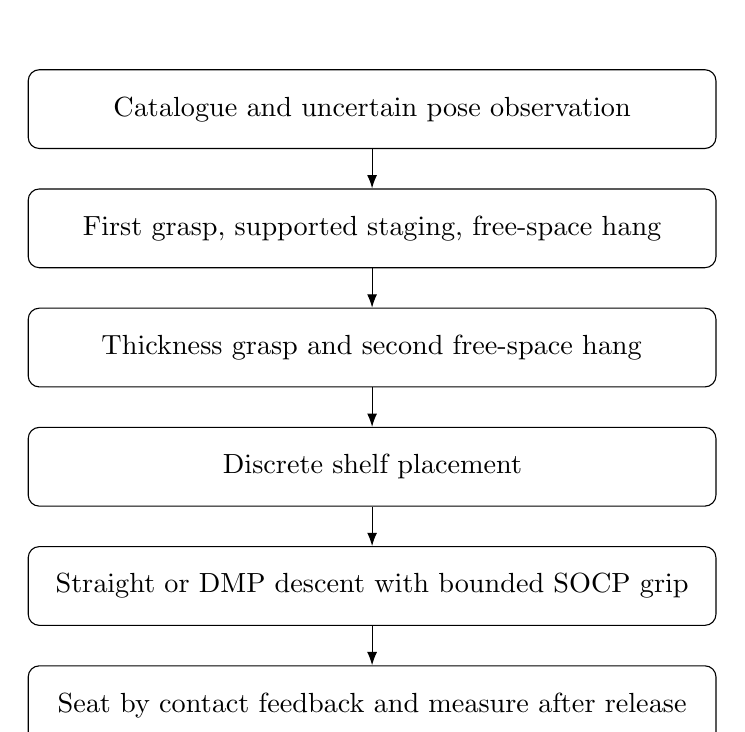
\begin{tikzpicture}[>=Latex,box/.style={draw,rounded corners,align=center,text width=85mm,minimum height=10mm},node distance=5mm]
\node[box] (a) {Catalogue and uncertain pose observation};
\node[box,below=of a] (b) {First grasp, supported staging, free-space hang};
\node[box,below=of b] (c) {Thickness grasp and second free-space hang};
\node[box,below=of c] (d) {Discrete shelf placement};
\node[box,below=of d] (e) {Straight or DMP descent with bounded SOCP grip};
\node[box,below=of e] (f) {Seat by contact feedback and measure after release};
\foreach \u/\v in {a/b,b/c,c/d,d/e,e/f}{\draw[->] (\u)--(\v);}
\end{tikzpicture}
\caption{The catalogue insertion chain. The DMP acts during descent. The grasp estimator and force allocator retain their separate roles. Supported staging is not an airborne estimation manoeuvre.}
\label{fig:tetris-chain}
\end{figure}

\thesisfigure{ch10_tetris/pipeline_snapshots.png}{One move of the chain in the full simulation (seed 7025, move 3, an L). The piece arrives flat and is grasped on its silhouette, rolled up about its bottom edge and put down in the nest, grasped again across its thickness, held still in the air while the wrench is read, carried to the mouth of the slot and seated.}{fig:tetris-snapshots}

\thesisfigure{ch10_tetris/nest_poses.png}{Every piece of the same game standing in the nest before the thickness grasp. The I is spawned upright in the nest and the station stands the O; the other five are stood up by the two tools.}{fig:tetris-nest}

\section{The quasi-static insertion model}

Let $u\in\R^3$ contain the two planar command coordinates and the in-plane angle. Let $z$ contain object and contact-proxy coordinates. The model potential has control, resistance and contact terms,
\begin{equation}
W(z,u)=W_{\mathrm{ctrl}}+W_{\mathrm{resist}}+W_{\mathrm{contact}}.
\end{equation}
For the reciprocal object coordinates, equilibrium is represented by $W_z=0$. If $W_{zz}$ is invertible in the neighbourhood, differentiation gives
\begin{equation}
\frac{dz}{du}=-W_{zz}^{-1}W_{zu}.
\end{equation}
The reduced command-force derivative is the Schur complement
\begin{equation}
\mathcal G=W_{uu}-W_{uz}W_{zz}^{-1}W_{zu}.
\label{eq:haptic-metric}
\end{equation}
The subscripts denote derivative row and column spaces. This ordering is dimensionally consistent when $z$ has more coordinates than $u$.

The implementation follows the equilibrium manifold with relaxation,
\begin{equation}
\dot z_o=-W_{zz}^{-1}\bigl(W_{zu}\dot u+\eta W_z\bigr),
\end{equation}
for the object coordinates. Contact proxies use a separate nonreciprocal potential and relaxation law. Their dynamics are not obtained by treating every proxy as an ordinary elastic degree of freedom in the same symmetric Hessian.

The model uses smooth superellipse contact geometry to obtain the required derivatives. A sharp-edged simulator body can create a face contact that this model does not represent in the same way. Model-to-simulator agreement must therefore be tested at the level of geometry and load paths, not only at the level of an ordinary differential equation.

\subsection{Where the insertion load comes from}
\label{sec:insertion-load-source}

The scene model and the force allocator answer different questions. The nominal scene specifies the incoming piece, the shelf, the neighbours and their poses. Along a candidate route, the contact model determines which surfaces meet and the wrench that their interaction applies to the piece. The reduced model above is one proposal mechanism; the exported Kinova routes use the load saved during a replay in the full apparatus simulation. This gives a path-indexed nominal environment wrench $\vect w_{\mathrm{ext}}^{\mathrm{nom}}(s)$, where $s$ denotes route progress.

At the stated object pole, quasi-static balance requires
\begin{equation}
\vect b(s)=-\vect w_g-\vect w_{\mathrm{ext}}^{\mathrm{nom}}(s),
\label{eq:insertion-load-source}
\end{equation}
with all moments transported to that same pole. The SOCP then asks how the two hands can supply $\vect b(s)$ through their six pad contacts. It does not calculate collisions with the shelf itself. A stored resisting-load convention may absorb the minus sign into the exported quantity; the balance and the moment pole, rather than a field name, fix the physical sign.

\begin{figure}[htbp]\centering
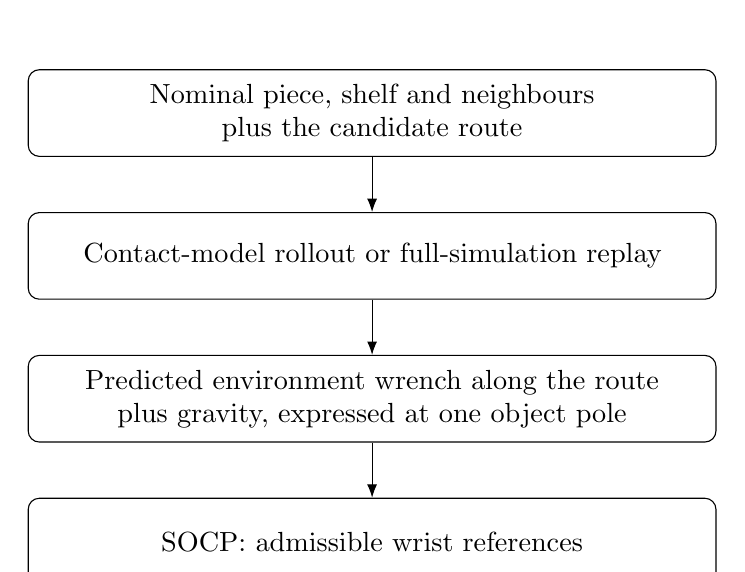
\begin{tikzpicture}[node distance=7mm,box/.style={draw,rounded corners,align=center,text width=85mm,minimum height=11mm},>=Latex]
\node[box] (scene) {Nominal piece, shelf and neighbours\\plus the candidate route};
\node[box,below=of scene] (contact) {Contact-model rollout or full-simulation replay};
\node[box,below=of contact] (load) {Predicted environment wrench along the route\\plus gravity, expressed at one object pole};
\node[box,below=of load] (allocation) {SOCP: admissible wrist references};
\draw[->] (scene)--(contact);\draw[->] (contact)--(load);\draw[->] (load)--(allocation);
\end{tikzpicture}
\caption{The source of the allocator's insertion load. Collision prediction belongs to the scene rollout. The SOCP distributes its requested load through a fixed local grasp model. The actual execution can meet a different contact when geometry or compliance differs.}
\label{fig:insertion-load-blocks}
\end{figure}

With an offline plan, this calculation is completed before the physical descent. The runtime interpolates the stored references and uses wrist measurements to regulate squeeze and detect excessive interaction. Such feedback does not make the stored collision prediction update itself. In an online variant the allocation is solved again using the current inputs, but it still requires an explicit estimate or prediction of the environment load. The comparison in Chapter~\ref{ch:kinova} uses the offline variant and keeps this distinction visible.


\section{Haptic distance}

If the reduced interaction force is $\vect f_u=W_u$, its local rate along equilibrium is $\dot{\vect f}_u=\mathcal G\dot u$. The interaction cost is
\begin{equation}
\phi=\int_0^T\norm{\mathcal G\dot u}\,dt
=\int_0^T\sqrt{\dot u^\top\mathcal G^\top\mathcal G\dot u}\,dt.
\label{eq:haptic-distance}
\end{equation}
For a symmetric $\mathcal G$, the integrand uses $\mathcal G^2$, as in the implementation. It measures the total variation of interaction force under the model, rather than mechanical work or maximum force.

This cost alone does not reward accurate final placement. It also decreases if a rollout is truncated early. The training code therefore treats a failed rollout as inadmissible instead of awarding it a small partial integral. Costs are meaningfully compared only when the compared trajectories satisfy the stated completion conditions.

\section{Dynamic movement primitives}
\label{sec:dmp}

The DMP has three command coordinates and twenty radial basis functions per coordinate. With canonical phase
\begin{equation}
s(t)=\exp(-\alpha_s t/\tau_0),
\end{equation}
the forcing term is
\begin{equation}
\vect f_{\Theta}(s)=s\frac{\Theta\vect\psi(s)}{\sum_j\psi_j(s)},\qquad
\psi_j(s)=\exp\left[-\frac12\left(\frac{s-c_j}{h_j}\right)^2\right].
\label{eq:dmp-forcing}
\end{equation}
The implemented state equation is
\begin{equation}
\frac{d}{dt}\begin{bmatrix}u\\v\end{bmatrix}
=\frac1{\tau_0}\begin{bmatrix}
v\\-K(u-u_g)-Bv+\vect f_{\Theta}(s)
\end{bmatrix},
\quad K=15I,\quad B=2\sqrt{15}I.
\label{eq:dmp-state}
\end{equation}
Here $v$ is the stored velocity-state coordinate; if $\tau_0\neq1$, it equals $\tau_0\dot u$. The inherited augmented implementation uses its default $\tau_0=1$, so the coordinate equals the physical command rate in those rollouts. A time-scaling change requires consistent use of that rate in the environment equation and haptic integral.

The weights $\Theta\in\R^{3\times20}$ provide sixty search variables. Zero weights give the reference attractor trajectory. Over a finite horizon it approaches, rather than reaches exactly, its target. The final physical seating stage is therefore not replaced by assuming the DMP endpoint is exact.

The analytic rollout uses an RK45 integration with relative tolerance $10^{-3}$, absolute tolerance $10^{-6}$, a nominal horizon of $1.5$ s and output spacing $0.002$ s. These are parameters of the inherited analytic model. The physical execution is paced separately to remain within the manipulation speed settings. Numerical integration time is not itself a measured industrial insertion time.

\section{Elitist search}

The black-box optimizer perturbs the current weights with Gaussian samples, evaluates rollouts, sorts them by cost and averages the best one per cent. The first rollout retains the unperturbed incumbent. For small rollout populations, the retained set contains a single candidate. This is elitist search, not a path-integral update or a covariance-adaptation algorithm.

The implementation uses a stable ordering for tied costs. When every rollout fails, the incumbent remains. Exploration scales for translation and rotation are stated separately because the coordinates have different units. Changing either is a comparison arm and must be recorded with the policy.

The Python port was checked against the MATLAB right-hand side at reference states, with a reported discrepancy of $9.2\times10^{-14}$. This is a numerical port check. It does not imply that the analytic contact model matches the shelf or that the learned trajectory transfers to the hands.

\section{Adapting the environment to tetrominoes}

A book row has neighbours with uniform profiles. A tetromino slot does not. Its flank can be occupied at one row and open at another. Its lower support can differ from column to column. The task-specific world construction therefore uses flank profiles by row band and support profiles by column.

A shelf wall is fixed. A neighbouring piece is an object that may move within the contact model. Giving both the same spring-supported state would make a wall artificially compliant. Omitting support below the incoming piece would make completion depend only on the DMP target rather than on seating.

The policy key records the piece, orientation and local environment profile. A route trained for one notch cannot be assigned to another merely because both are labelled ``piece on the left''. This increases the number of worlds but avoids a hidden geometry substitution.

\section{Keeping finite grip in training}

An analytic or simulator rollout can apply a command spring directly to the piece. That is an idealized handle. The real simulation apparatus instead has two compliant tools, six friction-limited contacts and a scalar squeeze loop. A route using a direct handle may depend on a load the finite grasp cannot carry.

The later training stage therefore executes each rollout with the actual tri-pad tools, allocator, jam detection, slow seating and release. The final placement error is measured after release. Force variation is measured on that apparatus rather than assumed equal to the analytic model's force history.

During insertion, a coupling displacement in the planar model produces additional force and moment demand. The wrapper maps its two translational coordinates into world directions and its angular demand into the current pad axis. Gravity compensation is added. The resulting desired wrench is passed to the same bounded force allocator used for holding.

This changes the role of squeeze. It must support weight and resist insertion load together. Increasing grip can help only within the friction and geometric conditions already discussed. A DMP that requires a large moment cannot be accepted simply because its path looks smooth.

\section{Persistent grasp error and played boards}
\label{sec:persistent-grasp-error}

Training on a shifted start point moves the command trajectory relative to the environment. It does not reproduce a piece that remains displaced and rotated inside the hands while those hands believe a nominal grasp. The later robustness training introduces this persistent relation error throughout the descent.

The saved recipe tests four prescribed combinations with magnitudes $6$ mm across the slot, $3^\circ$ in the shelf plane and $10$ mm along insertion. The values were selected from the 75th-percentile component errors of eighty-four recorded grasps. Four scenarios are a finite stress test; they are not all eight sign corners of a three-variable box and not a probabilistic guarantee over the full error distribution.

The recipe first evaluates the straight reference. If every scenario seats within $12$ mm, it saves a straight-line marker. Otherwise, a five-rollout, five-generation search starts from the better reference and stops once all tested scenarios meet the target. The retained route is compared with the straight and model references on the worst-scenario placement, with force variation used for close outcomes.

A placement-error term with weight $0.5$ N/mm is added to the interaction cost in the simulator training. This is an application-specific modification to the analytic haptic objective and must be named as such. Failed insertions rank below successful ones. A low integral cannot compensate for an unseated piece.

Only boards satisfying the trainer's declared cleanliness conditions are used for local policy refinement. This is a training-data selection, not a filter for the whole-game evaluation. Held-out game results must include failure to reach later worlds, accumulated placement drift and missing-library fallbacks.

\section{Established observations and current limitations}

The saved process summary reports thirty placed pieces out of forty-two on the six training seeds with the earlier library and thirty-seven out of forty-two with the persistent-error library. Its reported comparison gives $p=0.29$. The result is a training-seed observation, not a statistically established held-out improvement.

The earlier unseen-seed comparisons were close or inconsistent. Their interpretation is constrained by library coverage: many requested insertion worlds had no apparatus-validated route and used a model policy or straight fallback. Overall game performance therefore combines local route quality, library coverage and the errors left by previous moves.

Exact enumeration of the nominal $6\times6$ planning task in the saved analysis gives $5040$ seven-piece orders, $4942$ distinct planned games and $2491$ world keys. These are counts under that planning definition. Physical drift can produce additional distinct states, and changes in the key definition can change the count. Enumeration is not a completed insertion campaign.

The frozen September ledger contains $379$ identified policies or straight markers, of which $96$ remain above the $12$ mm worst-scenario target. Of those, $23$ are at least $60$ mm from target. These are library triage counts, not success rates for the newer friction or grasp configuration.

\thesisfigure{ch10_tetris/tetris_shoulder_case.png}{An unresolved S-piece insertion case from a saved diagnostic comparison. A shoulder meets a neighbouring top edge. Both displayed routes leave the piece above the intended seat, illustrating why a trajectory change must be evaluated with the actual shelf contact geometry. The image is retained unchanged; it is not a successful-run illustration.}{fig:tetris-shoulder}

Figures~\ref{fig:insertion-forces} and~\ref{fig:insertion-same-route} show what the apparatus measures during an insertion. They come from two games on the same seed, one with the learnt routes and one with the straight line on every move; the first placed seven pieces of seven and the second three. On the first move the board is identical in the two games, and the straight line seats closer than the learnt route ($1.0$ against $3.7$ mm). On the fourth move both games drive the same straight route, because the learnt one had not beaten it in training, into boards that differ by at most $2.3$ mm and $0.8^\circ$ per neighbour. One Z seats at $4$ mm and the other ends $123$ mm out. Neither detected a jam. The difference in that game comes from the board left by earlier moves, not from the route.

\thesisfigure{ch10_tetris/insertion_forces.pdf}{One insertion on the same board, straight line against learnt route (seed 7025, move 1, an S). Top: normal force measured by each hand and the target set by the SOCP. Middle: horizontal push of the slot on the piece, measured from the pads in quasi-statics, and the push predicted by the model along the route. Bottom: moment carried about the pad axis, the channel held by the tri-pads' friction alone.}{fig:insertion-forces}

\thesisfigure{ch10_tetris/insertion_forces_same_route.pdf}{The same straight route into two boards that differ by millimetres (seed 7025, move 4, a Z). Where the piece ends out, the two hands stop delivering the same squeeze and the slot push grows to $5$ N; where it seats, the moment about the pad axis peaks at $0.5$ Nm instead.}{fig:insertion-same-route}

The ongoing September campaigns combine a central-grasp change with effective pad friction increased from $0.49$ to $1.0$. One saved board-specific result reaches the target at all four scenarios, but the two changes have not been separated. It cannot be attributed to the DMP, grasp location or friction alone.

\section{Insertion into slots narrower than the piece}
\label{sec:tight-slots}

The game-level evaluation above uses the slots that the placement rule produces. With a $3$ mm seam and pieces that end a few millimetres from their cells, most of those slots offer positive or nearly zero lateral clearance. The straight reference route seats in many of them, and in that regime a learned route can only avoid contacts that a straight descent would also avoid. This does not test the case for which the haptic planning method was designed. In the book case study of Yang et al.~\cite{yang2025haptic}, the gap between the neighbouring books is half the thickness of the book being inserted. The object cannot enter along a straight line; the trajectory has to tilt, push and slide so that the neighbours move and make room. The remainder of this chapter focuses on that regime, transferred to tetrominoes in the shelf, and keeps the complete apparatus of the previous chapters in the loop.

\subsection{Constructing narrowed slots from played boards}

A narrowed slot is not drawn by hand. Each case starts from a board reached in a recorded game, just before the move in question, so that every neighbour has the pose and the support it actually had. The slot is then narrowed by moving the neighbours sideways, never by changing the incoming piece.

On every side of the slot that is flanked by another piece, the neighbour column that already protrudes furthest towards the incoming piece defines the face of that side. All pieces on that side, together with every piece resting on them, are translated by one common horizontal displacement so that this face enters the incoming piece's silhouette by a fixed intrusion $\delta$, measured against the piece column it faces at the same height. Moving the whole side by one amount preserves the relative arrangement of the neighbours; translating them one by one would make stacked neighbours interpenetrate. A shelf panel is never moved and an open flank stays open.

The case studied here uses $\delta=15$ mm per side, one eighth of a cell. For the I piece standing in a single column, the opening becomes $90$ mm for a $120$ mm piece, which gives the name ``$75\%$'' to this set. The same intrusion in millimetres is used for every shape, rather than the same fraction of the piece width, so that a two-cell-wide piece is not asked to displace its neighbours twice as far.

A narrowed board is accepted only if it remains physically consistent: no moved piece may overlap a piece that was not moved, enter a side panel, or lose its support. These are preconditions on the board, computed from the modelled geometry before any insertion is attempted; they are not predictors of success. Boards that appear twice in the archive and near-identical cases, with the same insertion type and the same moved neighbours, are counted once.

The selection covers every tetromino and, for each, aims at insertions of different type. The type of an insertion is defined by the rotation of the piece, the kind of flank on each side (piece, panel or open) and what the piece lands on (shelf floor or another piece). Within each tetromino the cases are chosen so that they differ in as many of these attributes as the archive allows.

\subsection{The apparatus during the insertion}

The insertion is executed by the same apparatus as the rest of the pipeline. The piece is held across its thickness by the two compliant tri-pad tools of Chapter~\ref{ch:contacts}. At every control tick the squeeze is set by the convex program of Chapter~\ref{ch:socp}, with the friction cones~\eqref{eq:friction-cone} as hard constraints and the per-pad limit~\eqref{eq:pad-cap} inside the program. The cost carries the human coordination prior of Chapter~\ref{ch:prior}, queried at the current attitude of the piece, so the distribution of contact forces between the two hands follows the same TP-GMM/GMR precision used when the piece is held in the air. The desired wrench passed to the program combines gravity with the insertion load predicted by the coupling displacement of the route, as described in the previous sections.

The descent follows the learned route at the manipulation pace of the earlier chapters. A jam detector compares the measured contact load with the load the route predicts and stops the push when they diverge. A slow seating stage closes the remaining depth by contact feedback, and the piece is released before its placement error is measured. A route is therefore evaluated on where the piece rests after it has been let go, not on where the hands believed it was.

The physical parameters of this study are declared, not tuned to the outcome. The effective pad-to-piece friction coefficient is set to $1.0$, a coating with higher friction than the $0.49$ used elsewhere in this thesis; piece-to-piece friction is $0.5$ and piece-to-floor friction $0.3$. The contact of the seated pieces is compliant, with stiffness $8000$ N/m and damping $207$ Ns/m. The jam detector is relaxed so that the route is allowed to push. Each of these values belongs to the experimental condition and is recorded with every result.

\subsection{Searching a route that makes room}

The route is the dynamic movement primitive of Section~\ref{sec:dmp}, and its weights are searched with the elitist procedure described above. Each candidate is first integrated through the quasi-static model, which turns the sixty weights into a command path for the hands. That path is then executed by the apparatus in the full simulation, and the cost is computed from the execution. For a candidate that seats, the cost is the total variation of the externally applied force measured on the piece during the route, plus a placement term of $0.5$ N per millimetre of final error. A candidate that does not seat is ranked below every seated candidate, by how close it came to the seat. Without that ranking, every failed candidate would tie and the search could not move when no candidate seats yet, which is the normal situation at the start in a narrowed slot.

The search used for these slots is wider than the one inherited from the book study, with Gaussian perturbations of standard deviation $3$ on the translational weights and $40$ on the rotational ones, and it starts from the better of the straight route and the analytic model's own policy for that piece. Since the slot is already narrower than the piece, the training and evaluation use the nominal grasp. The persistent grasp errors of Section~\ref{sec:persistent-grasp-error} are not superimposed on the intrusion; in the earlier configuration they were, with four persistent combinations scored on the worst.

\thesisfigure{ch10_tetris/learnt_routes.pdf}{Three learnt routes into narrowed slots, retrained at the size of the laboratory pieces ($100$ mm cubes, $70$ mm tri-pad). The piece is drawn at eight points of its route, the black line is the path of its centre, the red cells are the slot and the dashed line is the straight descent. Placement is measured after release in the full simulation.}{fig:learnt-routes}

\subsection{A reduced contact model as a fast proposal stage}

A rollout on the full apparatus costs about half a minute of simulation, and a complete search costs several hours per slot. To reduce this cost, the search can be split in two stages: a fast proposal stage in a reduced quasi-static model, followed by a short refinement on the full apparatus that starts from the proposed route.

The reduced model keeps the structure of the haptic model of Yang et al.---super-ellipse bodies, corner-against-surface contacts with a proxy on the surface, the coupling to the hands and the relaxation dynamics along the equilibrium manifold---and changes what the tetromino shelf requires:
\begin{itemize}
\item The incoming piece is the union of its catalogue columns, each a super-ellipse rigidly attached to one piece frame. The frame origin is the centroid of the cells, as in the analytic model, so that a route found in the reduced model can be used directly as a starting point for the full search.
\item Each neighbour is a rigid body with a single horizontal coordinate. A piece standing on the shelf does not lift or tilt while it is pushed sideways; the floor and the side panels are fixed.
\item Contacts are created only between columns that can come within reach of each other, including the columns lying under the piece. Neighbour-to-neighbour, neighbour-to-panel and piece-to-floor contacts are one-sided springs along a single direction and need no proxy.
\item Friction is Coulomb at every contact. A proxy sticks while the tangential force stays inside the cone and slips only by the excess,
\begin{equation}
\dot q=\frac{r}{\norm{\partial_q\sigma}}\,\frac{\mathrm{dz}\!\left(f_t,\ \mu f_n\right)}{k_c},
\end{equation}
where $\sigma(q)$ is the surface point of the proxy, $f_n$ and $f_t$ the normal and tangential components of the contact spring force, $k_c$ the contact stiffness, $r$ a relaxation rate and $\mathrm{dz}(f,c)$ a smoothed dead zone that vanishes for $\lvert f\rvert<c$. The inherited implementation drives the proxy towards the corner irrespective of the cone, so its friction depends on the speed rather than on the normal load.
\item Each neighbour is held by friction on what it stands on, with a breakaway force that grows with the load the incoming piece applies to it from above,
\begin{equation}
F_k=F_{k,0}+\mu_{\mathrm{under}}\,N_k^{\downarrow},
\end{equation}
where $F_{k,0}$ is the breakaway of the free neighbour and $\mu_{\mathrm{under}}$ is the floor or piece-to-piece coefficient. A piece pressed from above therefore resists sliding more, as it does in the full simulation.
\item The grasp can slip: the hands are coupled to a grasp point that slides on the piece once the force exceeds $2\mu F$ or the moment about the pad axis exceeds $4\mu F R_{\mathrm{tri}}$, with $F$ the squeeze that the convex program delivers on that board in the full simulation.
\item The DMP is integrated at a time scale that keeps its peak speed at the descent speed of the apparatus, so the path is the same as at the original time scale and only its duration changes.
\item A candidate that drives any body more than $15$ mm into another is discarded as non-physical.
\end{itemize}

\thesisfigure{ch10_tetris/lean_to_pybullet.pdf}{One route through both stages (J piece, narrowed slot, nominal grasp). Top: the route found in the reduced model, seated at $0.5$ mm. Bottom: the same route driven in the full simulation with the two tri-pads, the SOCP squeeze, the jam detector and the slow seat; it seats at $4.5$ mm with $2$ mm of slip in the pads, so the refinement stopped at its first rollout. On other slots the reduced model was more lenient than the full simulation and its route did not transfer.}{fig:lean-to-pybullet}

The reduced model is used only to propose routes. Its cost is the distance from the seat at the end of the rollout, and the proposed route becomes the starting point of a short search on the full apparatus, with the same cost, settings and evaluation as above. Every number reported for this study is measured on the full apparatus; the reduced model's own outcome is not used as evidence of a successful insertion.

\todo{Report the narrowed-slot campaign: per piece and per insertion type, the straight route against the searched route on the full apparatus, placement after release, grasp slip, neighbour displacement and jam events; the proposal-plus-refinement scheme against the search on the full apparatus alone, including simulation time spent.}

\section{Final validation still required}

\todo{Freeze the policy library, code revision, contact friction, grasp selector, world-key definition and fallback before the final held-out comparison. Do not aggregate a moving training ledger into a final result.}

\todo{Separate the central-grasp change from the friction change on the same boards. State physical and optimization friction values, including any deterministic cone margin.}

\todo{Evaluate straight, analytic-model and apparatus-trained routes on the same held-out seed set. Report policy coverage, actual route selected, local insertion completion and whole-game placement outcomes. Preserve failures and unreachable later moves.}

\todo{Report placement after release, maximum interaction force, accepted allocation fraction, jam events and grasp slip. Explain how often improved local placement prevents a subsequent failure. Use games as the independent unit for game-level comparisons.}

\todo{Verify the slow-execution assumption from measured velocities and inertial/contact-wrench ratios during descent and seating. Retain the supported staging as an explicitly different stage from free-space identification.}

\subsection{Towards two Kinova arms}

The insertion stage has been packaged for two Kinova Gen3 arms as a ROS~2 package that depends only on the route files, the convex program and the arm interface. Each route is exported from its replay in the full simulation as the commanded object path, the predicted slot load and the grasp pose. Played offline without physics, the package reproduces the commanded flange path of the simulation to $0.2$ mm median and $0.6$ mm maximum. The routes were retrained at the size of the laboratory pieces, $100$ mm cubes and a $70$ mm tri-pad: $27$ of $29$ narrowed slots and $12$ of $15$ five-piece kit slots seat in simulation. With the shelf floor $0.35$ m below the arm bases, every route pose lies $564$--$816$ mm from the shoulder, inside the $902$ mm reach. The laboratory tool is two printed plates with a central spring and a sponge layer; its pad friction and its hand--piece stiffness must be measured before any route is trusted on it. The first executions on the two arms, with force/torque sensors at the wrists, are reported in Chapter~\ref{ch:kinova}.

The industrial analogy is shelf replenishment with finite contact capacity and imperfect pose information. The useful outcome would be a route that creates space without losing the grasp and leaves neighbours in a usable state. The present evidence establishes the modelling and evaluation requirements for that outcome; the final held-out campaign is still needed to quantify it.


\chapter{Insertion on Two Kinova Gen3 Arms}
\label{ch:kinova}

This chapter executes the insertion stage of Chapter~\ref{ch:tetris} on two physical arms. The convex program, the scalar squeeze loop, the jam sentry and the learnt routes are transferred from simulation; the arm dynamics and passive tool determine how their commands are realized. Each wrist carries a six-axis force/torque sensor, so the hand wrenches that the controller closes on are measured rather than estimated from joint torques.

The first hardware series was recorded on 21 and 22 October 2026, with the piece presented by hand and the board assembled from the route file. Its ten executions over four worlds are reported with the operator's recorded outcomes. A later series of 23 October uses offline normal-force feedforward plus integral feedback. It is presented separately, followed by comparisons with an articulated Gen3 simulation and a test of the laboratory impedance source.

\section{The cell}

Two Kinova Gen3 7-DoF arms stand with parallel bases $600$ mm apart. A shelf stands in front of them, as in Fig.~\ref{fig:kinova-cell}. Its floor runs from $120$ to $770$ mm ahead of the bases and lies $30$ mm below the base plane. The shelf is $125$ mm deep and has no front or back panel, so each tool reaches one face of the piece from its own side. All poses are expressed in the shelf frame of the simulation: origin on the floor at the far end of column~$0$, $z$ up, the shelf plane is $x$--$z$ and the pad axis is $y$. Each arm's base pose in that frame was measured by hand.

\thesisfigure[0.62]{ch11_kinova/cell_top_view.pdf}{The cell from above, in the frame of the right base. The two tools are drawn at the grasp of the T route; the piece moves in the mid-plane of the shelf, between them.}{fig:kinova-cell}

The pieces are built from $100$ mm polystyrene cubes; a whole tetromino weighs $50$ g. The routes were trained at this size (Chapter~\ref{ch:tetris}): the five-piece kit worlds with the slot narrowed to $75\%$ and the route starting with the piece's grasp point at $800$ mm, and the narrowed worlds of the column-$2$--$5$ set.

Each tool is, from the flange outwards: an ATI Mini40 (SI-80-4) force/torque sensor with its adapters, a free coil spring and a printed tri-pad of three spheres of $15$ mm radius on a $70$ mm triangle. The front of the spheres is $100$ mm from the flange. The spring is $50$ mm long, with an axial stiffness of $2700$ N/m, and is not guided. In series with a $1000$ N/m arm it gives about $730$ N/m per hand along the squeeze axis. Its estimated torsional stiffness is about $0.25$ Nm/rad, against $20$ Nm/rad at the wrist. The spring therefore passes forces but almost no moment about the pad axis, which matters for the twist channel below. The $150$ g mounted on each flange are included in the URDF used for gravity compensation.

\begin{table}[htbp]\centering\small
\caption{The hardware configuration of the runs of 21--22 October 2026.}\label{tab:kinova-setup}
\resizebox{\textwidth}{!}{\begin{tabular}{@{}ll@{}}
\toprule
Arms & 2 $\times$ Kinova Gen3, 7 DoF, bases parallel, $600$ mm apart \\
Arm control & Cartesian impedance at the flange, joint torque at $1$ kHz \\
Stiffness, damping & $1000$ N/m, $20$ Nm/rad; $5$ N\,s/m, $1$ Nm\,s/rad \\
Wrist sensors & ATI Mini40 SI-80-4, Ethernet NetBox, $1$ kHz, means of 5 at $200$ Hz \\
Tool & sensor, free spring ($2700$ N/m), tri-pad; $100$ mm, $150$ g past the flange \\
Pieces & $100$ mm polystyrene cubes, $50$ g per tetromino \\
Command loop & both flange targets from one object frame, $100$ Hz \\
Squeeze and twist & closed on the measured hand wrenches, every $20$ ms \\
Convex program & re-solved every $100$ ms in a worker thread \\
Speed & route, turns and seat $3\times$ slower than trained \\
Safety stops & $60$ N per hand, $40$ mm tracking, jam sentry, sensor silent $50$ ms \\
\bottomrule
\end{tabular}}
\end{table}

\subsection{Control on the arms}

Each arm runs the laboratory's Cartesian impedance controller: a target flange pose in, joint torques out at $1$ kHz, with gravity compensated from the URDF. The stiffness is diagonal in the base axes and fixed at launch. The values in Table~\ref{tab:kinova-setup} are those used in the bimanual friction-margin experiments on the same arms~\cite{frictioncone2026}, not the $1500$ N/m and $40$ Nm/rad of the simulated wrist.

The insertion node runs one loop at $100$ Hz. It reads both flange poses by forward kinematics and both sensor readings, and sends both flange targets. As in simulation, the targets follow from one commanded object frame plus a scalar squeeze along the pad axis. Every $20$ ms the squeeze is integrated on the measured normal force towards the convex program's target. With the full wrench enabled, the opposite twist of the two flanges about the pad axis is integrated on the measured moment error as well. The convex program is re-solved every $100$ ms. On the robot computer it takes a median $47$--$58$ ms, so it runs in a worker thread: the loop keeps streaming targets with the last solution until the next one arrives.

\subsection{The implemented Cartesian impedance}
\label{sec:kinova-impedance}

The insertion node commands absolute end-effector poses. The laboratory controller turns each pose into seven joint torques; it does not impose that pose kinematically. Let $\vect q_K,\dot{\vect q}_K$ be the position and velocity returned by the joint-state Kalman filter. An additional first-order low-pass filter gives
\begin{equation}
\dot{\vect q}_{f,k}=\alpha_k\dot{\vect q}_{K,k}+(1-\alpha_k)\dot{\vect q}_{f,k-1},
\qquad \alpha_k=\frac{\Delta t_k}{(2\pi f_c)^{-1}+\Delta t_k},
\quad f_c=100\ \mathrm{Hz}.
\end{equation}
The Kalman filter uses a constant-acceleration model and wrap-aware position innovations. Both filters precede the velocity feedback in the impedance law.

In the arm base axes, define the pose error and Cartesian velocity as
\begin{equation}
\vect e=\begin{bmatrix}\vect p_d-\vect p\\\operatorname{log}(R_dR^\top)^\vee\end{bmatrix},
\qquad \vect v=J(\vect q_K)\dot{\vect q}_f,
\end{equation}
where $J$ is the end-effector Jacobian with world-aligned axes at the end-effector pole. The implemented torque before limiting is
\begin{equation}
\vect\tau_0=J^\top\bigl(K\vect e-D\vect v\bigr)
-B\dot{\vect q}_f+\vect g(\vect q_K)+\vect\tau_{\mathrm{fric}}.
\label{eq:kinova-impedance}
\end{equation}
The diagonal matrices $K,D$ set the Cartesian stiffness and damping. The term $\vect g$ compensates gravity from the arm-and-tool URDF. This implementation has no Coriolis feedforward term. The optional null-space stiffness is zero in the configuration considered here.

The source configuration used for the later comparison sets translational stiffness to $1500$ N/m and rotational stiffness to $20$ Nm/rad, with damping $60$ N\,s/m and $7$ Nm\,s/rad. Joint damping is $B=0.001$ Nm\,s/rad. These are distinct from the settings recorded for the initial series in Table~\ref{tab:kinova-setup}. The Stribeck friction option is enabled, but its scale defaults to zero and is not overridden by the inspected launch; its nominal feedforward contribution is therefore zero. This does not imply that physical friction is absent.

The controller clips each joint torque to $35$ Nm on joints 1--4 and $12$ Nm on joints 5--7. The surrounding node then limits its change to $0.5$ Nm per control tick. A joint speed above $2$ rad/s for twenty ticks triggers a gravity-only mode. The nominal control rate is $1$ kHz, while joint states and the joint-torque wrench estimate are published at $250$ Hz. The node uses measured time increments, capped at three nominal control periods; these nominal rates do not remove scheduling delay.

The torque-based wrench estimate is a separate signal from the ATI measurement. With the source's reaction-torque convention, $\vect\tau_{\mathrm{sensor}}=-\vect\tau_{\mathrm{motor}}$, its quasi-static expression is
\begin{equation}
\hat{\vect w}_{\mathrm{EE}}=(J_{\mathrm{local}}^\top)^+
\bigl(\vect\tau_{\mathrm{sensor}}+\vect g+\vect\tau_{\mathrm{fric}}\bigr).
\label{eq:kinova-wrench-estimate}
\end{equation}
It is expressed in the end-effector local frame. Unmodelled inertia, friction and gravity residuals can enter that estimate. The ATI instead measures the mechanical wrench at its own sensor pole; changing pole and axes is required before comparing components.

\begin{figure}[htbp]\centering
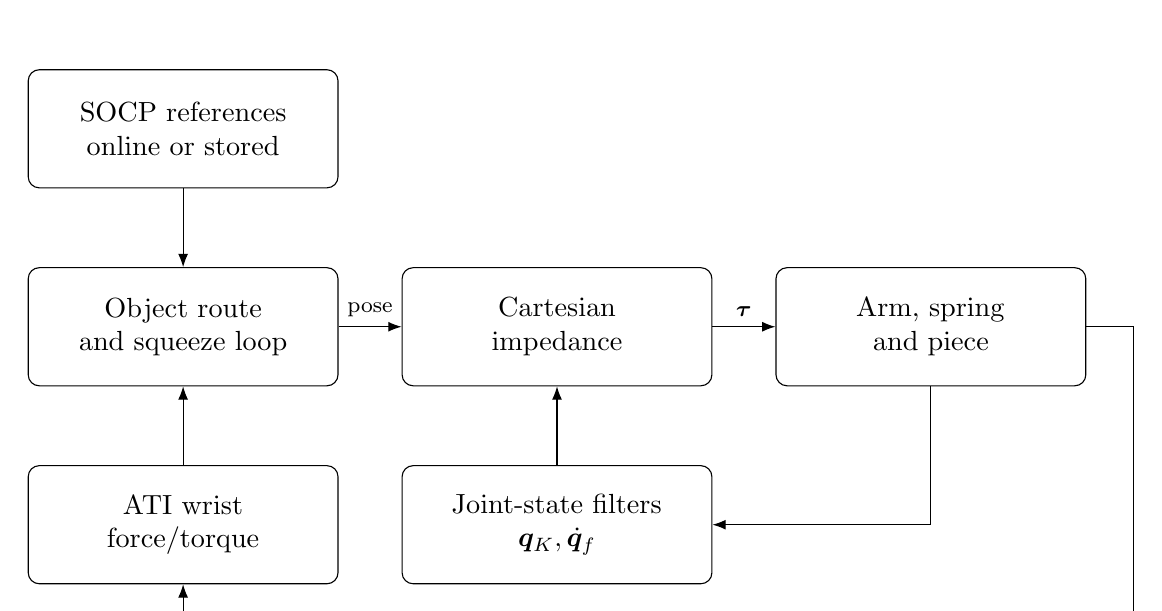
\begin{tikzpicture}[node distance=10mm and 8mm,box/.style={draw,rounded corners,align=center,text width=37mm,minimum height=15mm},>=Latex]
\node[box] (outer) {Object route\\and squeeze loop};
\node[box,right=of outer] (inner) {Cartesian\\impedance};
\node[box,right=of inner] (plant) {Arm, spring\\and piece};
\node[box,above=of outer] (plan) {SOCP references\\online or stored};
\node[box,below=of inner] (state) {Joint-state filters\\$\vect q_K,\dot{\vect q}_f$};
\node[box,below=of outer] (ati) {ATI wrist\\force/torque};
\draw[->] (plan)--(outer);
\draw[->] (outer)--node[above,font=\footnotesize]{pose}(inner);
\draw[->] (inner)--node[above,font=\footnotesize]{$\vect\tau$}(plant);
\draw[->] (plant.south) |- (state.east);\draw[->] (state)--(inner);
\draw[->] (plant.east) -- ++(6mm,0) |- ([yshift=-5mm]ati.south) -- (ati.south);
\draw[->] (ati)--(outer);
\end{tikzpicture}
\caption{The two control levels. The outer loop adjusts a pose to regulate squeeze; the inner loop realizes that pose compliantly through joint torque. Joint-state feedback sets the impedance damping, while the ATI closes the outer force loop. The passive pads have no independent force actuators.}
\label{fig:kinova-control-blocks}
\end{figure}

Equation~\eqref{eq:kinova-impedance} is a conventional local impedance structure. Its damping term opposes measured Cartesian velocity; increasing $D$ changes this inner mechanical response, not an arbitrary time delay in an outer-loop model. Whether it suppresses a particular force oscillation depends on the arm dynamics, filters, tool compliance and contact state. The damping comparison below therefore keeps the force controller fixed and states which inner realization was simulated.


\subsection{The wrist sensors}

Each NetBox streams at $1$ kHz; a light reader publishes means of five samples at $200$ Hz, and the loop averages the samples of its own period. The sensor's pose follows from the flange pose and a fixed rotation. That rotation was found by three holds by hand per arm: nothing touching, a press on the pad face towards the flange, and a press down on the front of the tri-pad. The two measured force directions fix the sensor axes against the flange axes, and the moment of the downward press fixes the sign. The two sensors turned out to be rotated by about $9^\circ$ and $12^\circ$ about the flange axis. At each tare, with the tools in free air, the bias is the mean of $0.5$ s of samples less the tool's weight at the current attitude, so the weight is removed again at every attitude afterwards. The standard deviation at rest was below $0.03$ N per force axis in every run.

\section{What the arms were asked to do}

Each run follows the sequence of Chapter~\ref{ch:tetris}. The piece is presented by hand between the open tools at the route's grasp pose, above the board. The tools close until contact and squeeze, and the operator lets go. The pair then carries the piece to the mouth of the slot and along the learnt route. A slow straight seat follows, then a descent until the shelf is felt to carry the piece, the release, and a retreat. The commanded path is the one exported from the full simulation, scaled to the real cell, at one third of the trained speed.

\thesisfigure{ch11_kinova/planned_vs_executed.pdf}{The four worlds executed, as built: neighbours, the piece where it is presented (solid) and its slot (dashed). The dashed black line is the route's planned path of the grasp centre, the midpoint of the two pads. The coloured lines are the measured midpoint of the two flanges in every run of that world, from the mouth of the slot to the seat.}{fig:kinova-routes}

Figure~\ref{fig:kinova-routes} shows the four worlds. The T is presented turned by $8^\circ$ from its slot attitude, the L and the Z by $3^\circ$, the S upright; each route turns the piece into its slot attitude on the way down.

\section{What they did}

Table~\ref{tab:kinova-runs} lists the ten runs, all with the full wrench and the wrist sensors as the source of the hand wrenches. Every run followed its route, found the seat and released the piece, with no jam stop. The operator recorded eight insertions and two entries; in the first T run the neighbouring L was not pushed aside, in the second all neighbours were. The placement error, the worst cell against its target as the simulation scores it, has not yet been measured by hand.

\begin{table}[htbp]\centering\footnotesize
\caption{The runs of 21--22 October 2026. Asked and measured: the median normal force per hand while carrying (target of the convex program and wrist sensor). Side: the largest horizontal force the environment exerted on the piece. Twist: the largest rotation the twist channel added to a flange. Solve: median time of one convex program on the robot computer.}\label{tab:kinova-runs}
\setlength{\tabcolsep}{4pt}
\resizebox{\textwidth}{!}{\begin{tabular}{@{}llrrrrrrrl@{}}
\toprule
Piece & Date, time & Route & SOCP ok & Asked & Measured & Side & Twist & Solve & Outcome \\
 & & [s] & & [N] & [N] & max [N] & max [$^\circ$] & [ms] & \\
\midrule
T & 21/10 20:15 & 18.9 & 207/208 & 4.8 & 4.7 & 0.8 & 1.4 & 56 & entered; L not pushed \\
T & 21/10 20:28 & 18.9 & 209/210 & 4.8 & 4.8 & 1.4 & 1.8 & 55 & inserted; neighbours pushed \\
T & 21/10 20:34 & 18.9 & 209/210 & 4.9 & 4.8 & 1.4 & 1.6 & 57 & inserted \\
S & 22/10 12:45 & 15.4 & 307/308 & 3.9 & 3.9 & 4.7 & 1.4 & 47 & entered \\
S & 22/10 13:48 & 15.4 & 309/309 & 3.9 & 4.0 & 4.5 & 2.3 & 49 & entered \\
L & 22/10 15:00 & 22.0 & 234/235 & 4.8 & 4.9 & 1.3 & 2.5 & 51 & inserted \\
L & 22/10 15:07 & 22.0 & 235/236 & 4.9 & 4.9 & 0.8 & 2.8 & 52 & inserted \\
L & 22/10 15:12 & 22.0 & 233/233 & 4.8 & 4.8 & 1.4 & 1.9 & 52 & inserted \\
Z & 22/10 15:20 & 19.1 & 204/204 & 4.4 & 4.3 & 2.4 & 2.4 & 58 & inserted \\
Z & 22/10 15:28 & 19.1 & 203/204 & 4.4 & 4.4 & 2.4 & 3.6 & 58 & inserted \\
\bottomrule
\end{tabular}
}
\end{table}

\paragraph{Tracking.} The measured midpoint of the flanges stays within a median $5$--$8$ mm of its commanded position, at most $14$--$21$ mm, while carrying. This error includes the compliant response under contact load and possible gravity-model residuals; the logs do not separate their contributions. Close to the route start, a $0.77$ m reach with the tool horizontal, inverse kinematics on the controller's URDF finds the flange up to about $9$ mm short of the commanded pose of the T route: the start pose is at the edge of the arms' workspace, and the impedance absorbs the difference as tracking error.

\paragraph{Squeeze.} The squeeze closed on the measured force follows the convex program. The median normal force per hand differs from its target by at most $0.1$ N in every run (Table~\ref{tab:kinova-runs}). The targets are $3.9$--$4.9$ N per hand for a $0.49$ N piece, and the largest measured value is $8.0$ N. Figure~\ref{fig:kinova-wrench} shows one run of the L. During the route the target varies with the predicted slot load and the measured force follows it, with oscillations of about $1$ N at roughly $1$ Hz. A compliant arm--tool chain can support such motion, but these traces alone do not distinguish mechanical resonance, feedback dynamics, contact changes and measurement effects. The small median bias is not an instantaneous $0.1$ N tracking bound.

\thesisfigure{ch11_kinova/wrench_one_run.pdf}{One run of the L (22 October, 15:00), from contact to release; the time the arms held still waiting for the operator is cut out. Background: approach and squeeze (grey), carry to the mouth (blue), route (sand), slow seat and seat by feel (green), release (grey). From the top: normal force of each hand measured by its wrist sensor against the target of the convex program; the force the environment exerts on the piece, with the jam limit (off the scale during the route, about $40$--$60$ N); the moment each hand applies about the pad axis; the twist correction added to each flange.}{fig:kinova-wrench}

\paragraph{Contact with the board.} The horizontal force the environment exerted on the piece stayed below $5$ N in every run, far under the jam limit; the S pushed hardest. In Fig.~\ref{fig:kinova-wrench} the vertical force rises to $4.5$ N at the seat: this is the shelf taking the piece, the event the seat-by-feel step waits for.

\paragraph{Twist.} The twist channel was active in every run, but it had little to act on. The moment each hand applied about the pad axis stayed within $\pm0.04$ Nm. Meanwhile the correction rotated the flanges steadily, up to $1.4$--$3.6^\circ$, without reducing that moment. This is what the spring predicts: at about $0.25$ Nm/rad, $2.5^\circ$ of flange rotation changes the moment at the pads by about $0.01$ Nm. With this tool the opposite twist cannot be regulated through the flange. The insertions succeeded with the squeeze carrying the piece, and the twist channel contributed at most a small rotation. A tool that transmits torsion, or a twist actuated at the pad, would be needed before the channel can be evaluated.

\paragraph{The convex program.} Out of $203$--$309$ solves per run, at most one failed; that historical implementation fell back to the trained pickup squeeze for that tick. This describes the recorded series, not the later allocator-failure policy. A median solve of $47$--$58$ ms within a $100$ ms period was enough once the program left the streaming loop. Solved inline, the same program had stalled the loop for $40$--$260$ ms about once per second during carrying, and the arms visibly jerked.

\paragraph{Why the wrist sensors.} Earlier runs used the external wrench estimated from the joint torque sensors. With the arms empty, that estimate drifted by up to $8$--$9$ N per arm along a route, repeatably. Each route needed an empty-handed recording of the error, subtracted at the nearest flange position, and the moments could not be corrected that way. Figure~\ref{fig:kinova-ati-est} compares the two sources on the same run. During the route, the estimate departs from the sensor by up to about $4$ N. After the release, it settles at $-1.5$ to $-2.5$ N where the sensor reads zero. These errors are of the size of the squeeze itself.

\thesisfigure{ch11_kinova/ati_vs_estimate.pdf}{Normal force of each hand in the run of Fig.~\ref{fig:kinova-wrench}: the wrist sensor, which the controller used, against the joint-torque estimate logged beside it (tared at the same instant).}{fig:kinova-ati-est}

\section{Earlier runs with the joint-torque estimate}

Before the wrist sensors were mounted, the same insertion ran with the joint-torque estimate and the empty-handed correction. On 16 October the T was inserted with the scalar squeeze; the Z entered, but the stack of neighbours half fell. That run used the correction recorded for the T, not for the Z. On 19 October the L was inserted. On 20 October the T of the column-$2$--$5$ set was the first insertion with the twist channel enabled. It was inserted, but not smoothly. Its log shows the two hands opposing each other vertically instead of sharing the weight, with the measured forces needing more friction than the model's $\mu=1$ in two thirds of the ticks. These runs established the sequence on the arms and showed the limits of the estimate that the wrist sensors removed.

\section{The later feedforward-plus-integral series}
\label{sec:kinova-ffi}

The archive of 23 October contains twelve recorded successful FFI runs: three each for Z, L, S and T. This is a selected set of completed executions, not a denominator for a hardware success rate. These runs use normal-force feedforward with a bounded ATI integral correction and an offline SOCP plan. They are a later condition than the online full-wrench series above; changing the gains, allocation schedule and feedback together prevents attributing a difference to any single change.

At each planned sample, the allocator still computes a complete wrench pair. The normal-only execution extracts a common per-hand demand
\begin{equation}
N^*=\max\left(1\ \mathrm{N},\ \sum_j\lambda_{Lj},\ \sum_j\lambda_{Rj}\right).
\end{equation}
This runtime scalar selection is distinct from the signed-distance constraints inside the SOCP. It does not mean that every pad is given a separate $1$ N normal-force floor. The remaining optimized force and moment components are logged, but are not all tracked by this scalar loop.

Let $N_0$ be the measured per-hand preload at pickup. Relative to the frozen pickup poses, the requested extra closure of each hand is a feedforward displacement plus an integral trim:
\begin{align}
\delta_{\mathrm{ff}}^*&=\frac{N^*-N_0}{k_{\mathrm{eff}}}, & k_{\mathrm{eff}}&=680\ \mathrm{N/m},\nonumber\\
e_N&=2N^*-(N_L+N_R), &
\delta_{I,k+1}^{\mathrm{trial}}&=\delta_{I,k}+k_I e_N\Delta t_k,
\label{eq:kinova-ffi}
\end{align}
with $k_I=0.0016$ m/(N\,s). The error is the sum over both hands. Feedforward receives priority within the feasible motion interval; the retained integral state is the attainable trim, which prevents windup against the limits. Trim travel is bounded by $\pm3$ mm per hand and total extra closure by $\pm12$ mm. Both trim and total speed are limited to $2$ mm/s per hand. Force updates are nominally every $20$ ms; elapsed-time limiting handles delayed updates. No additional moving average or derivative action is introduced in this condition.

The first two runs of each piece were frozen as development data and the third chronological run as holdout before controller exploration. The comparisons below use the first development Z and L runs, identified in Appendix~\ref{app:reproducibility}; they do not tune against or claim prediction of the holdout. Real force samples are used for plotting afterwards, never to drive the simulated piece.

\section{An articulated Gen3 simulation beside the measurements}
\label{sec:kinova-sim-comparison}

Two articulated seven-joint Gen3 models are placed using the laboratory base transforms, with the shelf, incoming piece and neighbouring pieces in the nominal route geometry. Forward kinematics is checked against an independent chain and the logged initial poses. This checks the frame construction, not the accuracy of the hand-measured laboratory transforms. The setup initializes the open grasp pose and represents the operator's support until release; the physical homing and hand presentation are not replayed.

The tool model has a $2700$ N/m central axial spring and three pad springs of $500$ N/m each. These parallel paths give a total small-deflection axial stiffness of $4200$ N/m between the mount and plate; setting the central spring to $2700$ N/m does not set the complete tool to that value. The $150$ g tool mass is split into $110$ g rigidly attached and $40$ g mobile beyond the virtual sensor. Piece mass is $50$ g and pad friction is $\mu=1$. Environment contacts use $8000$ N/m stiffness and $207$ N\,s/m damping.

The inherited lateral and rotational tool parameters are also assumptions. In particular, the central model retains $40$ Nm/rad torsional stiffness before the pad contribution, far above the approximately $0.25$ Nm/rad estimated for the free laboratory coil. The model therefore cannot validate the real twist authority. Neither actuator transmission dynamics nor measured hardware timing and force noise are identified from these runs.

\subsection{Two inner-controller realizations}

The complete insertion curves use a locally implicit Cartesian impedance approximation with the same nominal $K=1500/20$ and $D=60/7$. It includes articulated inertia, gravity and Coriolis compensation, a small null-space damping term and the URDF torque limits. Its integration and limiting differ from Equation~\eqref{eq:kinova-impedance}; it does not reproduce the laboratory Kalman, slew and watchdog chain. The outer FFI and the nominal SOCP planner are the original implementations. This condition tests their interaction with the declared mechanical model, rather than a byte-identical robot servo.

A separate trial executes the hardware-free laboratory controller classes, including the Kalman and RC filters, gravity term, torque clip, slew and speed watchdog. The executable torque and wrench-estimation methods match the reference supplied for the laboratory controller. The copied full-file version is frozen, but its identity with the file actually deployed on the NVIDIA computer has not been independently verified. Matching controller equations is distinct from matching the physical plant.

The virtual wrist measurement comes from the fixed-joint mechanical reaction, with the mobile tool's gravity removed. It is kept separate from the joint-torque estimate of Equation~\eqref{eq:kinova-wrench-estimate}. The simulated signal is block-averaged through the declared sensor and outer-loop sampling chain. It is not replaced by the SOCP target or by a measured laboratory waveform.

\subsection{Normal forces and wrist moments}

Figure~\ref{fig:kinova-real-sim-force} shows the first Z and L development runs beside the autonomous simulations. Each clock starts at its own departure towards the slot mouth. No force-based time warping or amplitude fitting is applied. The same axis limits are used within each pair, and the recorded controller inputs are plotted without additional display smoothing. The target is the original per-hand SOCP reference, including its variations.

\thesisfigure[1.0]{ch11_kinova/real_sim_normal.pdf}{Measured normal force per hand: real ATI data (left) and articulated PyBullet with approximate inner impedance (right). Blue is left, orange right; the dashed line is the per-hand SOCP target. Rows are Z and L. Vertical dotted lines mark execution-stage changes on each run's own clock. These are two selected completed cases, not a controlled hardware--simulation validation population.}{fig:kinova-real-sim-force}

\thesisfigure[1.0]{ch11_kinova/real_sim_zoom.pdf}{The Z comparison on identical time and force scales, $12$--$17$ s after departure towards the mouth. The laboratory signal contains larger repeated fluctuations than this nominal simulation. A varying target and changing contacts remain present; these fluctuations cannot all be classified as sensor noise.}{fig:kinova-real-sim-zoom}

For quantitative comparison, let $\bar N=(N_L+N_R)/2$ and $e=\bar N-N^*$. Metrics use only the route stage, except for the separately reported seating excess. Both traces are interpolated on their own uniform $100$ Hz grids for metric calculation. Band RMS is obtained with a third-order Butterworth band-pass applied forwards and backwards. This offline analysis filter is not part of the controller. In particular, the force-band RMS contains target-driven motion as well as residual fluctuation; the band RMS of $e$ is also retained in the evidence.

\begin{table}[htbp]\centering\small
\setlength{\tabcolsep}{4pt}
\begin{tabular}{@{}llrrrr@{}}\toprule
Piece & Source & RMSE $e$ & $\bar N$, 0.8--2.5 Hz & $\bar N$, 2.5--10 Hz & Seat excess\\
& & (N) & RMS (N) & RMS (N) & (N)\\\midrule
Z & Real & 0.301 & 0.125 & 0.066 & 1.446\\
Z & Simulation & 0.209 & 0.042 & 0.014 & 0.850\\
L & Real & 0.282 & 0.115 & 0.066 & 2.638\\
L & Simulation & 0.278 & 0.043 & 0.012 & 1.470\\\bottomrule
\end{tabular}
\caption{Descriptive comparison of the two selected cases. All columns concern the mean of the two hands. Seat excess is $\max e$ during slow seating and seating by feel. RMS is not peak-to-peak amplitude, and a small median bias does not imply the same instantaneous tracking precision.}
\label{tab:kinova-real-sim}
\end{table}

The simulation is smoother in both bands, but its tracking error does not vanish. The L route RMSE is nearly the same as in the real run despite smaller repeated fluctuations. At seating, the measured peak excess of the mean force is $1.45$ N for Z and $2.64$ N for L, versus $0.85$ and $1.47$ N in the model. Route tracking and seating transients must therefore be reported separately.

\thesisfigure[1.0]{ch11_kinova/real_sim_moment.pdf}{Magnitude of the wrist moment, real (left) and simulated (right), on the same selected Z and L executions. These are sensor wrenches, not individual motor torques. The FFI condition regulates normal squeeze, not all three moments. Different tool compliance and sensor-pole construction limit the interpretation of amplitude differences.}{fig:kinova-real-sim-moment}

The simulated worst-cell errors after release are $4.41$ mm for Z at a $0.25$ ms physics step and $4.78$ mm for L at $0.5$ ms. Corresponding real worst-cell errors were not measured, so no placement-accuracy agreement is claimed. Moreover, the coarser Z simulation at $0.5$ ms ends $77.2$ mm from target. This step-size sensitivity is a failure of robustness of the current model and must accompany its finer-step result.

\subsection{What increasing damping to 80 changes}

The paired damping test changes only the approximate inner translational damping from $60$ to $80$ N\,s/m; rotational damping stays at $7$ Nm\,s/rad. The FFI gains, motion limits, geometry, SOCP profile and each case's physics step are fixed. In Z the route force RMS at $2.5$--$10$ Hz falls from $0.0138$ to $0.0117$ N; in L it falls from $0.0118$ to $0.0107$ N. The lower-band RMS remains about $0.042$ and $0.044$ N, respectively. Route RMSE remains about $0.209$ N for Z and $0.278$ N for L, and seating excess changes little.

This is evidence of a modest reduction of faster fluctuations in that model, not evidence that $D=80$ cures the laboratory oscillation. The full-source trial described next does not reach insertion at either damping value. A hardware comparison that changes only $D$, with the same FFI plan, repeated route and tool, is still needed to isolate the damping effect.

\subsection{The original-source trial and the predictive limit}

With the laboratory controller classes, the nominal articulated plant does not maintain the initial free-space pose. In the trial with a settled Kalman covariance and a $0.25$ ms physics step, the right-arm speed watchdog first triggers at $72$ ms and the left at $89$ ms; an external pose-error sentinel ends the trial at $0.12$ s, before pickup. Figure~\ref{fig:kinova-lab-source-stop} preserves the measured virtual wrist signals up to that stop. No insertion RMSE or seating overshoot can be assigned to this trial.

\thesisfigure[0.92]{ch11_kinova/original_source_stop.pdf}{Virtual wrist force and moment magnitudes during the original-source trial, before pickup. Tool gravity has been removed, while inertial reactions remain. Dotted lines mark the two speed-watchdog events. The run stops at $0.12$ s; no force curve is extrapolated beyond it.}{fig:kinova-lab-source-stop}

The kinematic, Jacobian and gravity comparisons were checked before interpreting this failure. A separate rigid-URDF Pinocchio forward-dynamics test also triggers the speed watchdog in free space under a small initial perturbation, including at finer steps. Thus pad contact and the Bullet contact solver alone do not explain the discrepancy. The available evidence does not identify which actuator, inertia, friction, internal filtering or deployed-parameter difference is responsible. The robot's demonstrated ability to hold in the laboratory is not reproduced by this plant.

The defensible conclusion is narrower than either ``the controller is validated'' or ``the motors cause the sinusoids''. The nominal approximate model completes the two selected insertions and exposes finite tracking error and seating overshoot. The original-source realization exposes an unresolved plant mismatch even before contact. Predicting hardware oscillations requires first reproducing a measured free-space hold and a small pose change with synchronized joint positions, velocities, commanded and measured torques, and timing. Until then, the smoother simulation is an explanatory comparison, not a causal reconstruction of the laboratory force trace.


\section{What these runs show and what they do not}

The initial series shows that routes learnt in simulation can be executed by two impedance-controlled arms following one object frame, while a squeeze loop closes on wrist-sensor measurements. Its small median force bias coexists with repeated fluctuations and larger transient errors. The later FFI series gives recorded scalar-force executions, but it is not a paired ablation of the earlier full-wrench condition.

The articulated simulations make the distinction between allocation and realization explicit. An admissible SOCP reference still has to pass through pose tracking, tool deflection and changing shelf contact. The approximate model can complete selected routes with smoother forces, yet its step-size sensitivity and the original-source free-space failure prevent using it to identify the cause of the real oscillations. Raising damping to $80$ has only a modest effect in the completed approximate simulations.

Real placement accuracy and neighbour displacement remain unmeasured. The passive spring gives the twist channel little authority in the initial apparatus. A controlled same-route comparison, changing only inner damping or only the outer force law, is needed before attributing improvements to one component. A synchronized free-space validation of the robot model must precede a claim that simulation predicts the hardware transients.

\todo{Measure placement after release and neighbour displacement; repeat a fixed route with identical FFI settings at two inner damping values; validate the free-space arm response with synchronized joint, torque and timing logs; evaluate twist only with a tool whose torsional transmission is measured.}

\chapter{Discussion and Conclusions}
\label{ch:discussion}

The framework links what the hands feel, what the system estimates and what the controller asks the contacts to transmit. Its strongest result is that these quantities depend on the same mechanics. Additional squeeze can deform the grasp. Additional compliance can preserve contact while suppressing the torsional measurement. A learned precision can then reward an apparatus-induced pattern rather than the intended human strategy.

\section{Grip force and geometry cannot be separated}

For fixed geometry and a fixed Coulomb coefficient, normal load increases the model's tangential-force bound. This mathematical monotonicity does not imply monotonic stability of a compliant grasp. The feasible set changes when the wrist moves or a pad detaches. The force ladder demonstrates that distinction on the documented case.

The design response is not simply to select a lower constant. It is to constrain effort, respect finite transmission and locate conformity in mechanical modes that do not unnecessarily disturb the grasp. The peripheral and central spring design makes those modes explicit. The force cap prevents requests outside the declared transmission range, while measured slack identifies a load the present contacts cannot carry.

This also changes the interpretation of fallback. A fallback is an independent control policy with its own setting and failure mechanisms. It cannot inherit the friction feasibility of a rejected allocation. Its use must be visible in the experiment record. A run dominated by fallback is not evidence that the optimizer successfully controlled it.

\section{The prior inherits its recording apparatus}

The session comparison shows that the same nominal manipulation can generate a different torsional covariance when the coupling stiffness changes. The valid prior is therefore tied to the recording gains, display scaling, saturation and contact conditions. It is not a detachable description of ``how humans manipulate boxes''.

The TP-GMM makes orientation adaptation possible, but its output retains the limits of the data. Isotropic vector scaling preserves rotation consistency. Products of Gaussians combine the two task frames. Mixture regression accounts for within- and between-component covariance. These operations are mathematically useful, but they do not enlarge empirical angular coverage or establish transfer to new contact mechanics.

The anchored grasp frame gives the transfer a meaningful coordinate system. Validation still requires the full, equal-trace identity and no-prior comparisons on the same apparatus. Until those comparisons are complete, the prior should be described as the implemented source of coordination preference rather than as a demonstrated cause of every successful grasp.

\section{Estimation should state what it does not know}

The vertical lift has a rank-two gravity regressor. This is an exact structural limitation. The unobserved component is not recovered by collecting more samples at the same orientation, nor should its covariance be set to zero by a pseudoinverse.

Observable-subspace least squares makes the distinction explicit. Slow orientation changes can add the missing direction, while acceptance checks reject samples inconsistent with the free-space model. Abstention is then a legitimate output. A system that records uncertainty and stops is more interpretable than one that returns a plausible number whose unsupported direction is hidden.

There are still model uncertainties beyond the implemented covariance: orientation error, contact-normal error, pole movement, correlated mass error and load paths outside the selected pads. Addressing them requires either measurement or a declared conservative model. A small regression residual does not prove that all such errors are small.

\section{Optimization and realization are separate tests}

The local convex program is well defined when its inputs are fixed. Its exact cones preserve the circular friction model; its force cost penalizes all contact directions; its cap bounds every pad; and its slack measures the unsupported part of the desired wrench.

The execution path does less than the mathematical allocator. It commands a scalar squeeze and relies on contact mechanics for the remaining distribution. This is an intentional practical interface, but it limits the claim. Force and moment tracking errors must be measured rather than assumed away. Full force allocation is a prediction until the realization layer is shown to reproduce it adequately.

No local optimum guarantees persistence of the contacts used to compute it. Nor does a successful simulation establish object-damage limits or industrial robot reachability. These belong to additional mechanics and system-level checks.

\section{What the industrial examples could resolve}

For mixed-content cartons, online load identification can replace a single assumed mass distribution. The useful benefit is not the estimator alone, but its effect on gravitational moment demand before reorientation. A controlled measurement can prevent an unsupported turn or request a different grasp.

For irregular rigid returns, discrete contact masks can prevent the controller from allocating force to a pad that never seated. Passive conformity can improve the contact set without lowering the upstream torsional recording stiffness. The corresponding deployment requirement is direct contact or wrist-wrench sensing, a defined friction range and an apparatus sized for the objects admitted to it.

For crowded shelf insertion, route learning can address a gap that cannot be entered by straight descent with the actual grasp error. Training on played boards exposes the route to neighbour drift. Training with the hands exposes it to finite friction and squeeze. Those two changes are necessary to evaluate the industrial analogy credibly.

These are possible mechanisms of benefit, not measured productivity improvements. The thesis provides no cycle-time, damage-rate or economic comparison with a deployed warehouse system. Such comparisons would need physical robot experiments, calibrated surfaces, repeated loads and a defined operating envelope.

\section{Limitations}

The human data are apparatus-specific and do not support a population-level behavioural conclusion. The valid prior has limited orientation coverage and an absolute load scale. The object mechanics are largely rigid, and the friction coefficient is treated as known within each arm. The allocator does not constrain all mechanical limits of the tool or arms.

The geometry campaign covers the blind-search regime only; rough-size and known-mesh planners were not implemented, and the information regimes are kept separate. It is a simulation: white sensor noise on the estimated wrench was tested and changes nothing, but sensor bias and drift were not modelled; there is one run per body, and twenty polytopes per face band, so the absence of a difference between tools on polytopes is not evidence of equivalence. Convex polytopes do not cover arbitrary nonconvex geometry. The plate can also introduce an extra contact unless its collision configuration is controlled: with a colliding plate it touched 69 of 80 polytopes and broke the estimate on most of them.

The catalogue Tetris task intentionally uses environmental support during staging and insertion. Its mass and geometry are known. It demonstrates reuse of the estimation equation and force allocator under different information, not proof that the complete blind pipeline works on tetrominoes.

The insertion library has incomplete coverage and unresolved worlds. The newer friction and grasp changes are confounded in current pilot outcomes. Final held-out effects cannot be stated until the frozen campaign is complete.

\section{Next experimental steps}

The force-realization audit, the deterministic deformation and jitter comparisons, a polytope population with audited blind decisions, and the same-population comparison of learned anisotropy, equal-trace isotropy and effort alone are now complete (Chapter~\ref{ch:geometry}). The remaining priorities for the geometry half are more polytopes per band, sensor bias and drift in the measured wrench, the rough-size and known-mesh planning arms, and repeated arrivals per body. The prior result, that its weight matters most and its learnt shape helps only slightly and only on polytopes, should be checked with a second prior model before it is generalised. For insertion, the necessary test is a frozen library evaluated on unseen games with coverage and cascaded placement error reported.

A physical passive-tool prototype would then test whether the simulated mode separation survives friction, manufacturing tolerances, travel limits and sensing noise. The stiffness matrix gives predictions for that test: axial support, low conforming tilt and a preserved torsional path. Those predictions should be measured as separate channels rather than compressed into one scalar stiffness.

\section{Conclusions}

The thesis develops a continuous chain from haptic recording to contact-constrained manipulation. Three discrete points per hand supply torsion through force lever arms. The two-frame prior supplies an orientation-dependent cost. Free-space gravity balance supplies inertial estimates with an explicit observability limit. The bounded allocator separates admissible contact forces from unsupported wrench demand.

The established measurements show why that chain must include the apparatus. Force can change geometry, and compliance can change the learned signal. Treating either as an independent tuning parameter can improve a visible outcome while invalidating the model used to explain it. The resulting design principle is to preserve the load path and measurement path first, then evaluate the estimator, prior and optimizer within that operating envelope.


\appendix
\chapter{Mathematical Checks}
\label{app:math}

This appendix collects direct identities used to check the implementation, rather than new general theorems. Methodological sources and separate code choices are identified in Appendix~\ref{app:reproducibility}. The numerical script tests frame transforms, moment regression, mixture covariance and the spring Hessian without running a campaign. Numerical agreement is not a physical success rate.

\section{Cross-product and moment signs}

For $\vect a=(a_x,a_y,a_z)^\top$,
\begin{equation}
\crossmat{\vect a}=\begin{bmatrix}0&-a_z&a_y\\a_z&0&-a_x\\-a_y&a_x&0\end{bmatrix}.
\end{equation}
This gives $\crossmat{\vect a}\vect b=\vect a\times\vect b$ and $\crossmat{\vect a}^\top=-\crossmat{\vect a}$. With contact force acting on the object, static balance about $\vect c$ is
\begin{equation}
\vect T_c=-(\vect p_c-\vect c)\times m\vect g
=m\vect g\times(\vect p_c-\vect c).
\end{equation}
The upright signs in Equation~\eqref{eq:planar-estimate} follow directly. A positive $r_x$ gives a negative contact moment about $y$ for downward gravity.

\section{Rotation and pole shift}

For a proper rotation $R$,
\begin{equation}
R(\vect a\times\vect b)=(R\vect a)\times(R\vect b),\qquad
\crossmat{R\vect a}=R\crossmat{\vect a}R^\top.
\end{equation}
Changing only coordinates sends $\vect F$ to $R^\top\vect F$ and $\vect T_c$ to $R^\top\vect T_c$. Changing the pole from $\vect c$ to $\vect d$ gives
\begin{equation}
\vect T_d=\vect T_c+(\vect c-\vect d)\times\vect F.
\end{equation}
The two transformations are tested separately. Rotating a wrist moment cannot replace shifting it to the estimated CoM.

\section{Equilibrium matrices and null spaces}

The global contact map has six rows and eighteen columns. Its null space contains force redistributions with zero net object wrench. The two-wrist map has twelve rows and eighteen columns, so it also has a nontrivial null space. Its kernel leaves each wrist wrench unchanged. In the previous allocator, whose decision variables were the pad forces, this kernel was invisible to the prior cost.

For a consistent fixed geometry, the object wrench can be obtained from the two wrist wrenches by shifting both to a common pole and summing. Therefore $G=AB$ for a fixed linear map $A$, and $\ker B\subseteq\ker G$. The converse generally fails. This distinguishes cost blindness from the broader definition of internal force.

In that previous allocator, adding $\gamma I_{18}$ to the contact-force Hessian, with $\gamma>0$, made the quadratic cost positive definite on every force direction; its effort term supplied this property after normalization, and a finite cap bounded the feasible set. In the active allocator the pad forces are feasibility witnesses outside the cost, and the cost is positive definite on the twelve wrist components it ranks.

\section{An upper bound is not a separate torsion constraint}

For equal contact radius $r$ and parallel normals,
\begin{equation}
|\tau_x|\leq\sum_i r\norm{\vect f_{t,i}}\leq\mu r\sum_i\lambda_i.
\end{equation}
Equality requires appropriately oriented tangential forces and can be prevented by simultaneous resultant-force demand. The allocator does not impose this bound as a replacement for six cones. It imposes the cones and computes the moment from their forces, retaining the coupling automatically.

\section{Observability identity}

Using $\crossmat{\vect g}^\top\crossmat{\vect g}=\norm{\vect g}^2I-\vect g\vect g^\top$,
\begin{equation}
H_k^\top H_k=R_k^\top\left(g_0^2I-\vect g\vect g^\top\right)R_k.
\end{equation}
It has two eigenvalues $g_0^2$ and one zero eigenvalue. The zero direction is $R_k^\top\vect g$. Repetition at one attitude multiplies the two nonzero eigenvalues but leaves the third zero. Distinct nonparallel directions make the intersection of kernels trivial.

The numerical check uses synthetic moments from a known first mass moment. Ground truth is appropriate here because this is an algebraic test outside any planner or controller decision. It checks recovery at full rank and confirms that the upright case does not recover the missing direction.

\section{Precision under a change of units}

Let $\vect d=S\vect d_n$ with invertible diagonal $S$. Then
\begin{equation}
\vect d^\top Q\vect d=\vect d_n^\top(S^\top QS)\vect d_n.
\end{equation}
If $C_n=S^{-1}CS^{-\top}$, its inverse is $Q_n=S^\top C^{-1}S$. This is the solver normalization. Multiplying precision by $S^{-1}$ instead would invert the intended unit correction.

For an isotropic vector block, scaling commutes with a rotation. The numerical check confirms that property and contrasts it with an axis-dependent scale. The latter is not prohibited for every statistical purpose; it is inappropriate for a model whose frame transformation assumes ordinary vector rotation after scaling.

\section{Conditional mixture covariance}

If component $k$ has conditional mean $\vect m_k$ and covariance $C_k$, and weights $\beta_k$, then
\begin{equation}
\operatorname{Cov}(\vect y\mid\vect x)=\sum_k\beta_kC_k
+\sum_k\beta_k(\vect m_k-\vect m)(\vect m_k-\vect m)^\top.
\end{equation}
The second term follows from the law of total covariance. For two components with equal within-component covariance but different means, it is strictly positive along the mean-separation direction. This test guards against a common implementation that returns only the averaged component covariance.

\section{Spring stiffness and the small-rotation approximation}

For attachment displacement $\Delta_i=B_i\vect\xi$, the quadratic energy is
\begin{equation}
U(\vect\xi)=\frac12\sum_i\vect\xi^\top B_i^\top K_iB_i\vect\xi.
\end{equation}
Its Hessian is $\sum_iB_i^\top K_iB_i$. A finite-difference Hessian of this same small-displacement energy should agree with the analytic matrix. That agreement checks the algebra and signs; it does not test large-angle mechanics.

For the axial-only triangle at its centre,
\begin{equation}
K_{\mathrm{axial}}=\diag\left(3k+K_c,0,0,0,\tfrac32kr^2,\tfrac32kr^2\right).
\end{equation}
The zero spring entries do not mean unconstrained motion in an actual prismatic-joint assembly. Joint constraints and contacts provide additional load paths. For the floating plate, lateral spring terms and the central six-dimensional spring must be added before deriving effective channels.

\section{Convexity conditions}

At a fixed contact geometry, the tangent projection is linear, compression is affine and the norm inequalities are convex. The prior Hessian is positive semidefinite after numerical projection, and effort is positive definite in the forces. Slack penalties are positive definite in slack.

These statements require unit normals and valid parameter ranges. A nonunit normal changes the tangent decomposition. Negative friction or an incompatible compression floor changes the admissible set. The source audit and numerical checks do not authorize omitting parameter validation in a final controller.

The quadratic objective can be converted to SOCP form through an epigraph. For example, $t\geq\norm{L\vect x}^2$ can be represented by
\begin{equation}
\norm{\begin{bmatrix}2L\vect x\\t-1\end{bmatrix}}\leq t+1.
\end{equation}
Thus the presence of a quadratic objective is consistent with conic canonicalization. It does not make the exact-friction problem a quadratic program with only linear constraints.


\chapter{Reproducibility and Evidence Status}
\label{app:reproducibility}

The manuscript is kept separate from the experiment folders. No controller, recording script, policy library or running campaign is changed during drafting. A source manifest records paths and SHA-256 hashes of the inspected implementation. This snapshot is necessary because the active project can change while its description is being written.

\section{Mathematical sources and implementation choices}

The manuscript distinguishes established methods, mechanical derivations, implemented choices and measured results. A citation supplies the background method; it does not prove that this apparatus meets its assumptions. Numerical identity checks likewise do not validate a physical manipulation.

\begin{longtable}{@{}p{0.27\textwidth}p{0.66\textwidth}@{}}\toprule
Topic & Origin and claim made here\\\midrule\endhead
UCM and task-equivalent variability & Scholz and Sch\"oner~\cite{scholz1999}; geometric metrics in Campolo et al.~\cite{campolo2013}. The wrench map specializes the idea to this task. The directional index is the project's statistic, not a universal UCM theorem.\\
Covariance and precision & Gaussian conditioning, inverse covariance and quadratic likelihood in Bishop~\cite[Sections 2.3 and 3.1]{bishop2006}. A precision-weighted control preference is an implementation choice; neural interpretation requires independent evidence~\cite{kutch2012}.\\
TP-GMM and GMR & Calinon~\cite{calinon2016}. Wrench outputs, gravity inputs, scaling, frame anchoring and regularization describe this implementation. Their effectiveness requires validation.\\
Gravity balance and identification & Static force and moment balance, also used in dual-arm estimation~\cite{wong2026}. Upright rank two follows from the cross-product matrix. Gates and unobserved-direction priors are code choices.\\
Convex allocation & Convexity and norm cones from Boyd and Vandenberghe~\cite{boyd2004}. Geometry, weights, caps, slack and realization are the implemented problem. No source proves a guarantee for uncertain, changing contacts.\\
Passive-tool stiffness & Local energy differentiation, informed by spring mechanics~\cite{herder2001,guest2006}. Stiffness values are calculated for this geometry, not measured on a physical prototype.\\
Insertion and DMPs & Source manipulation methods~\cite{yang2025haptic,yang2025multicontact}. Tetromino geometry, finite grasp, board state and error sampling are application adaptations.\\
Geometry and outcomes & Jitter and half-space sampling are synthetic test designs. Force ladders and reported statistics are project measurements, not conclusions from a background paper.\\
\bottomrule\end{longtable}

Appendix~\ref{app:math} makes signs, units and approximation boundaries inspectable through direct identities and local derivations. These are not new general theorems. Full-rank regression is identifiable under its model; sensor bias, elastic drift or support contact can still make it inaccurate.

\section{Implementation map}

\begin{longtable}{@{}p{0.28\textwidth}p{0.65\textwidth}@{}}\toprule
Thesis component & Source within the project\\\midrule\endhead
Haption recording & \sourcefile{lorenzo_code/Haption_Control/experiments/2_thesis_core/13-human_exploration_standardized_torsional.cpp}\\
Prior training & \sourcefile{lorenzo_data_analysis/07_torsional_ucm/C_prior_socp/25_prior_e_socp_sessione_C.py}\\
TP-GMM fitting and GMR & \sourcefile{lorenzo_data_analysis/04_tp_gmm_wielding/01_standardized_box/tpgmm_core.py}\\
Original bounded allocator & \sourcefile{lorenzo_data_analysis/07_torsional_ucm/lib/socp.py}\\
Passive-tool allocator & \sourcefile{lorenzo_data_analysis/10_tripad_passivo/lib/socp.py}\\
Array-based prior query & \sourcefile{lorenzo_data_analysis/10_tripad_passivo/lib/prior.py}\\
Observable-subspace estimator & \sourcefile{lorenzo_data_analysis/10_tripad_passivo/lib/estimator.py}\\
Axial-travel geometry & \sourcefile{lorenzo_data_analysis/10_tripad_passivo/lib/tool.py}\\
Floating plate & \sourcefile{lorenzo_data_analysis/10_tripad_passivo/spider_ee/floating_plate.py}\\
Contact-to-solver interface & \sourcefile{lorenzo_data_analysis/10_tripad_passivo/lib/convex.py}\\
Insertion allocation & \sourcefile{lorenzo_data_analysis/10_tripad_passivo/tetris/allocation.py}\\
Handling and grasp inversion & \sourcefile{lorenzo_data_analysis/10_tripad_passivo/tetris/handling.py}\\
DMP and search & \sourcefile{lorenzo_data_analysis/10_tripad_passivo/tetris/yl/dmp.py} and \sourcefile{yl/bbo.py}\\
Played-board training & \sourcefile{lorenzo_data_analysis/10_tripad_passivo/tetris/43_train_in_pybullet.py}\\
\bottomrule\end{longtable}

The passive-tool solver is a local counterpart of the bounded allocator. The mathematical chapter describes their common allocation, while recording the wrapper defaults that differ. The older force allocator supplies historical comparisons and prior-query functionality; it is not described as the current default solver.

\section{Evidence classes}

The manuscript uses four evidence classes. An implementation statement is checked against code. A measured statement is checked against a saved analysis or copied data table. An explanatory example is derived from declared synthetic geometry or an algebraic identity. A TODO specifies work required before an experimental claim can be made.

The figure manifest records the origin of every generated or copied asset. Model-query curves come from the saved prior. The observability figure uses prescribed attitudes. The directional-index figure reproduces reported values and intervals. The geometry gallery is illustrative and is not selected from successful grasps. The insertion image is a saved unresolved case retained unchanged.

\section{Data and configuration to freeze}

A final recording result needs the run identifiers, perturbation metadata, gains, display scales, saturation limits, drift filter and retained sample count. A final prior result needs the model file hash, training runs, component count, isotropic scales, regularization and empirical gravity coverage.

A final grasp result needs the body manifest, information regime, arrival-error distribution, tool variant, collision configuration, spring settings, friction values, force cap, compression floor, trajectory, estimator gates and fallback policy. These settings define the experiment. Omitting one can make two apparently similar rows represent different mechanical systems.

A final insertion result additionally needs the board snapshot, world key, policy hash, selected route, persistent-error scenarios, search settings, completion threshold, seating rule and post-release measurement time. A frozen library is distinct from a library being updated while games run.

\section{Ground truth and reporting}

Ground truth can construct the simulated body and calculate retrospective error. It cannot determine which objects enter a blind campaign, decide whether estimation is acceptable or select an action. The audit must include defaults and gates, not only direct parameters passed to the SOCP.

Catalogue Tetris is declared separately. Its known mass and geometry are legitimate task assumptions. Pose observation must still use the stated injected error, and the grasp inversion must use available tool signals rather than the body's true pose. Different information regimes cannot share a success-rate denominator without an explicit analysis of that difference.

\section{The Kinova comparison of 24 October}

The supplementary robot workspace is \sourcefile{kinova_dual_arm_dmp_insertion_fullwrench}. Its experimental archive \sourcefile{NVIDIA_RUNS/} is read-only. The analysis and simulations are stored under \sourcefile{docs/analysis_20261023/controller_night/pybullet_nominal_20261024/}; the thesis figure data are compact copies of the plotted signals with source hashes, not replacements for the original logs.

The selected real recordings end in \sourcefile{20261023_174143.csv} (Z) and \sourcefile{20261023_182743.csv} (L). They are the first development run of each piece. Their simulated counterparts are \sourcefile{Gen3_Z_central2700_implicit_dt025} and \sourcefile{Gen3_L_central2700_implicit_dt05}. The original-source trial is \sourcefile{Gen3Lab_Z_central2700_warm_dt025}; damping variants and all failed or coarse-step trials remain separately identified in the simulation archive.

The plotting script \sourcefile{figures/scripts/fig_kinova_comparison.py} reads the compact arrays in \sourcefile{figures/data/kinova_comparison_20261024/} and writes the four comparison figures. Its manifest identifies the original CSV and NPZ inputs by SHA-256, the simulation results and the copied laboratory-controller source. A separate metrics JSON records the stage masks, resampling and filter definition. The existing common plotting style supplies the serif typography and the same blue/orange hand colours as the earlier chapters. The three new block diagrams are TikZ source in the relevant chapters.

The frozen laboratory file has SHA-256
\begin{center}\footnotesize\ttfamily
685c80b14b527d450d6d42a03f779d04\\
f928a4e2d31d22b44c9733d7a98cbfba
\end{center}
Matching its executable methods to the supplied reference does not establish the identity of the entire deployed ROS node. This provenance limit and the original-source failure are retained beside the completed approximate simulations.


\section{Unfinished work}

The visible TODO paragraphs are part of the draft review process. They are not suppressed by a ``final'' switch that would leave unsupported prose looking complete. Before submission, each TODO should be resolved by adding evidence, narrowing the corresponding claim or deleting an unvalidated section.

The final length target is approximately 115 pages. The current text should grow through the missing controlled results, selected physical illustrations and their interpretation. Empty result pages, oversized plots and repeated background are not substitutes for those additions. The editorial page allocation is maintained outside the manuscript so that it does not become a scientific claim.

\todo{Complete the candidate and supervisor metadata, confirm the front-page requirements for the candidate's course cohort, and insert only an authorized university logo if required. The present layout is a clean UniGe-labelled adaptation, not a verified mandatory Robotics Engineering class file.}

\todo{Freeze the final experiment snapshot, rerun the mathematical and source checks, verify bibliography metadata and render the full manuscript. Inspect equations, figure labels, table widths and cross-references before submission.}


\backmatter
\bibliographystyle{unsrtnat}
\bibliography{references}


\end{document}

